
% !TeX encoding = UTF-8
% !TeX program = xelatex
% !TeX spellcheck = it_IT

\documentclass[noexaminfo,oneside,binding=0.6cm]{sapthesis}

\usepackage{enumitem}
\usepackage{polyglossia}
\usepackage{hyperref}
\usepackage[style=numeric]{biblatex}
\usepackage{csquotes}
\usepackage{subcaption}
\usepackage{amssymb}
\usepackage{float}
\usepackage{tabularx}
\usepackage{array}
\usepackage{booktabs}
\usepackage{multirow}
\usepackage{geometry}
\usepackage{linearb}
\usepackage{cypriot}
\usepackage{pifont}
\usepackage[linesnumbered,ruled,longend]{algorithm2e}
\usepackage{adjustbox}

\newcommand{\cmark}{\ding{51}} % ✓
\newcommand{\xmark}{\ding{55}} % ✗
\newcommand{\xxmark}{\ding{56}} % ✘ (heavier)

% --- Code listings ---
\usepackage{listings}        % main package for code
\usepackage{xcolor}          % colors for syntax highlighting
\usepackage[T1]{fontenc}     % proper encoding for monospace fonts
\usepackage{inconsolata}     % clean monospace font (better than default CM typewriter)

\setmainlanguage{english}
\setotherlanguage[variant=ancient]{greek}
\setotherlanguage{italian}
\newfontfamily\greekfont{Times New Roman}[Script=Greek]

\addbibresource{references.bib}


\hypersetup{pdftitle={An AI Framework for Linear B Translation into Ancient Greek and English},pdfauthor={Alessio Maiola}}


\title{An AI Framework for Linear B Translation into Ancient Greek and English}
\author{Alessio Maiola}
\IDnumber{1933744}
\course{Engineering in Computer Science}
\courseorganizer{Facoltà di Ingegneria dell'Informazione, Informatica e Statistica}
\AcademicYear{2024/2025}
\advisor{Prof. Aristidis Anagnostopoulos}
\authoremail{maiola.1933744@studenti.uniroma1.it}
\copyyear{2025}
\thesistype{Master Thesis}

\begin{document}

\definecolor{codegreen}{rgb}{0,0.6,0}
\definecolor{codegray}{rgb}{0.5,0.5,0.5}
\definecolor{codepurple}{rgb}{0.58,0,0.82}
\definecolor{backcolour}{rgb}{0.95,0.95,0.92}

\lstdefinestyle{mystyle}{
    backgroundcolor=\color{backcolour},   
    commentstyle=\color{codegreen},
    keywordstyle=\color{magenta},
    numberstyle=\tiny\color{codegray},
    stringstyle=\color{codepurple},
    basicstyle=\footnotesize\ttfamily,
    breakatwhitespace=false,         
    breaklines=true,                 
    captionpos=b,                    
    keepspaces=true,                 
    numbers=left,                    
    numbersep=5pt,                  
    showspaces=false,                
    showstringspaces=false,
    showtabs=false,                  
    tabsize=2
}

\lstset{style=mystyle}

\frontmatter
\maketitle
\dedication{Dedicated to \\ Luigi Ricci}


\begin{acknowledgments}

\end{acknowledgments}


\begin{abstract}
This thesis tests whether large language models (LLMs) can assist in translating Linear B administrative texts into Ancient Greek and English.
I build a compact \emph{Translation Pipeline} that couples brute-force cognate search with candidate aggregation, Linear-SVM auxiliary classifiers (part of speech, noun type, inflection), explicit handling of logograms/abbreviations, and structured multi-message prompting. Alongside the engineering, the thesis surveys the Aegean scripts (historical context, sites, linguistic features, and the decipherment of Linear B), details data collection (Linear A fragments, Linear B documents, Ancient Greek resources), and situates the approach within prior work on cognate matching and manual decipherment.

For cognates, I employed the generative \emph{NeuroDecipher} framework from Jiaming Luo and a brute-force extraction pass; for disambiguation, I add auxiliary labels and table-driven guidance.
Using Gemini~2.5~Flash, the system reconstructs plausible Ancient Greek forms and produces English translations for full tablets.
Evaluation against translations from Tselentis’ lexicon shows that automated translation is feasible: list-like inventories and administrative formulae are consistently recovered, vocabulary stays domain-appropriate, and English readings preserve the intended sense. An error taxonomy emerges: (i) weak/misleading cognates, (ii) case/number misassignment in context-poor lines, (iii) grammatical function errors from misclassification, and (iv) occasional logogram mishandling.
Greek reconstructions sometimes retain Mycenaean features, but these rarely obscure meaning.

I release code and data and outline concrete next steps: hand-curating auxiliary labels, enriching the logogram lexicon, adding a normalization stage toward Classical Greek, fine-tuning on expert-validated pairs, broader evaluation, and cross-script generalization (e.g., Cypriot syllabary vs. alphabetic Greek).

\end{abstract}

\tableofcontents

\mainmatter

\chapter{Overview of the Work}
This thesis introduces a pipeline for automating aspects of Linear B translation by combining probabilistic cognate matching, lightweight linguistic classifiers, and a prompted post-processing step.
The main components of the pipeline are:
\begin{enumerate}
    \item A cognate matching model, following Jiaming Luo \cite{luo}.
    \item Auxiliary classifiers that inform and constrain the decipherment: part of speech detection, noun type classification, and inflection detection.
    \item A prompt-engineering post-processor that proposes an Ancient Greek reconstruction and produces an English translation.
\end{enumerate}

\section{Chapters Overview}
Chapter \ref{chap:history} introduces the historical context of Aegean societies and their writing systems. Both Linear A and Linear B are outlined, together with the main stages of the Linear B decipherment.

Chapter \ref{chap:cognates} develops cognate matching, a core ingredient in computational decipherment. We formalize cognates and discuss matching principles grounded in proto-root similarity and phonological/morphological regularities.

Chapter \ref{chap:classifiers} presents the auxiliary tasks devised for this work and their models (part of speech detection, noun type classification, and inflection detection) together with the feature representations, training setup, and evaluation.

...
PALLE PALLE
... 

\section{Data Collection}
The data used in this work has been collected separately for Linear A, Linear B, and Ancient Greek.

\subsection{Linear A Fragments}
The Linear A fragments were collected from the corpora available at \url{https://sigla.phis.me} via web scraping.
Together with the fragments, site and document-level metadata were organized into a CSV with the following columns.

\paragraph{Field descriptions.}
\begin{itemize}
    \item \textbf{Site}: Archaeological site name (e.g., Arkhanes, Haghia Triada).
    \item \textbf{Number of Documents}: Total number of documents from that site in the  SigLA corpus (site-level count; repeated on each row for the site).
    \item \textbf{Document Name}: Canonical document identifier used by  SigLA (e.g., HT 117a, ARKH 1b); side labels a/b denote tablet faces.
    \item \textbf{Link}: Canonical URL to the  SigLA document page.
    \item \textbf{Type}: Document class (e.g., Tablet, Roundel).
    \item \textbf{Number of Signs}: Count of sign impressions recorded for the document (integer).
    \item \textbf{Number of Words}: Count of word tokens as segmented in the source (integer; can be 0 when only non-lexical marks are present).
    \item \textbf{Location}: Findspot within (or coincident with) the site when available; otherwise repeats the site name.
    \item \textbf{Period}: Archaeological period shorthand as in  SigLA (e.g., LM I, LM IB).
    \item \textbf{Motif}: Iconographic motif when applicable (common on roundels/seals; often empty for tablets), e.g., bull.
    \item \textbf{Width (cm)}: Maximum preserved width in centimetres (cm).
    \item \textbf{Height (cm)}: Maximum preserved height in centimetres (cm).
    \item \textbf{Depth (cm)}: Thickness in centimetres (cm).
\end{itemize}

\noindent\emph{Notes.} Missing values are left empty as in the source. Dimensions refer to the preserved object and follow  SigLA’s measurements (decimal separator “.”).

SigLA provides two parallel segmentations of each document: (i) a sign-by-sign view and (ii) a word/sequence view. The word view is not fully comprehensive: some isolated symbols are omitted and therefore never appear in the “words” export. For this reason, I keep the original sign segmentation as the authoritative layer, and use the word/sequence file to reconstruct identified sequences.

\paragraph{Signs CSV (per-sign records).}
Additional columns:

\begin{itemize}
  \item \textbf{Sign Number}: Running index of the sign within the document (starts at 1).
  \item \textbf{Sign}:  SigLA code of the sign (e.g., \texttt{ta}, \texttt{*118}, \texttt{AB16}, \texttt{[?]}).
  \item \textbf{Function}: Category of the sign (e.g., Syllabogram, Logogram) as given by  SigLA.
\end{itemize}

\paragraph{Words/Sequences CSV (per-word records).}
Additional columns:

\begin{itemize}
  \item \textbf{Sequence Number}: Running index of the sequence within the document (starts at 1).
  \item \textbf{Sequence}: Hyphen-separated syllabogram string exactly as in  SigLA (e.g., \texttt{a-su-mi-*118}).
  \item \textbf{Complete}: Boolean flag from  SigLA indicating whether the token is complete (True) or fragmentary/uncertain (False).
  \item \textbf{Length}: Number of syllabograms in the sequence (hyphen token count).
\end{itemize}

The algorithm used to reconstruct full documents, by aligning the sign and word sequences, is described in Algorithm \ref{alg:la-reconstruct}.

\begin{algorithm}[H]
\DontPrintSemicolon
\SetAlgoNoLine

\SetKwInOut{Input}{Input}
\SetKwInOut{Output}{Output}

\Input{For each document $d$: ordered $\mathrm{SIGN\_STREAM}_d = (s_1,\dots,s_m)$ by sign\_number; ordered $\mathrm{WORDS}_d = (w_1,\dots,w_n)$ where $w_j = (w_{j,1},\dots,w_{j,k_j})$ are syllables split by ``-''.}
\Output{$\mathrm{docs}[d]$: space-separated token stream.}

\ForEach{document $d$}{
  $\mathrm{out} \gets \langle\,\rangle$;\quad $\mathrm{buf} \gets \langle\,\rangle$;\quad $j \gets 1$;\quad $i \gets 1$\;

  \For{$t \gets 1$ \KwTo $m$}{
    \eIf{$j \le n \ \wedge\ s_t = w_{j,i}$}{
      \eIf{$i = k_j$}{ % full word
        emit $w_j$ as a complete word (syllables joined by "-") into $\mathrm{out}$;\quad
        $\mathrm{buf} \gets \langle\,\rangle$;\quad $i \gets 1$;\quad $j \gets \min(j{+}1,\,n)$\;
      }{
        append $s_t$ to $\mathrm{buf}$;\quad $i \gets i{+}1$\;
      }
    }{
      \If{$\mathrm{buf} \neq \langle\,\rangle$}{emit elements of $\mathrm{buf}$ into $\mathrm{out}$ in order;\quad $\mathrm{buf} \gets \langle\,\rangle$;\quad $i \gets 1$}
      emit $s_t$ into $\mathrm{out}$\;
    }
  }

  \If{$\mathrm{buf} \neq \langle\,\rangle$}{emit elements of $\mathrm{buf}$ into $\mathrm{out}$ in order}

  $\mathrm{docs}[d] \gets$ concatenate tokens of $\mathrm{out}$ with a single space
}

\caption{Align sequences $w_j$ to stream $(s_t)$: on full match emit $w_j$; else emit unmatched syllabograms.}
\label{alg:la-reconstruct}
\end{algorithm}

\subsection{Linear B Documents}
The Linear B corpus was similarly webscraped from the LiBER (Linear B Electronic Resources) archive \url{https://liber.cnr.it/tablet/list}.
However, the LiBER archive provides only a word-level segmentation, with no underlying sign-by-sign layer.
Because many Linear B documents are fragmented and carry annotations and uncertain signs, the data required cleaning to standardize the representation of extracted syllabograms.
The cleaned data was organized into three CSV files, as in the previous case.

The data of Linear B documents was organized as follows: the first CSV contains the document-level information, using the following fields.

\paragraph{Signs CSV (per-sign records).}Part of Speech
Additional columns:
\begin{itemize}
  \item \textbf{Sign Number}: Position of the sign within the document (starts at 1).
  \item \textbf{Sign}: Cleaned Linear B symbol (syllabogram / logogram / numeral / uncertain), e.g., pu, \texttt{M}, \texttt{1}, \texttt{[?]}.
\end{itemize}

\paragraph{Words/Sequences CSV (per-word records).}
Additional columns:
\begin{itemize}
  \item \textbf{Sequence Number}: Position of the word within the document (starts at 1).
  \item \textbf{Sequence}: Hyphen-separated cleaned symbols, e.g., \texttt{e-ri-sa-ta}, \texttt{M}, \texttt{1}.
  \item \textbf{Complete}: True/False flag from LiBER indicating whether the token is complete.
  \item \textbf{Length}: Number of syllabograms in the sequence.
\end{itemize}
The full webscraping and processing of Linear B data is detailed in Figure \ref{fig:webscrape-lb}.

\begin{figure}[H]
    \begin{adjustbox}{center}
        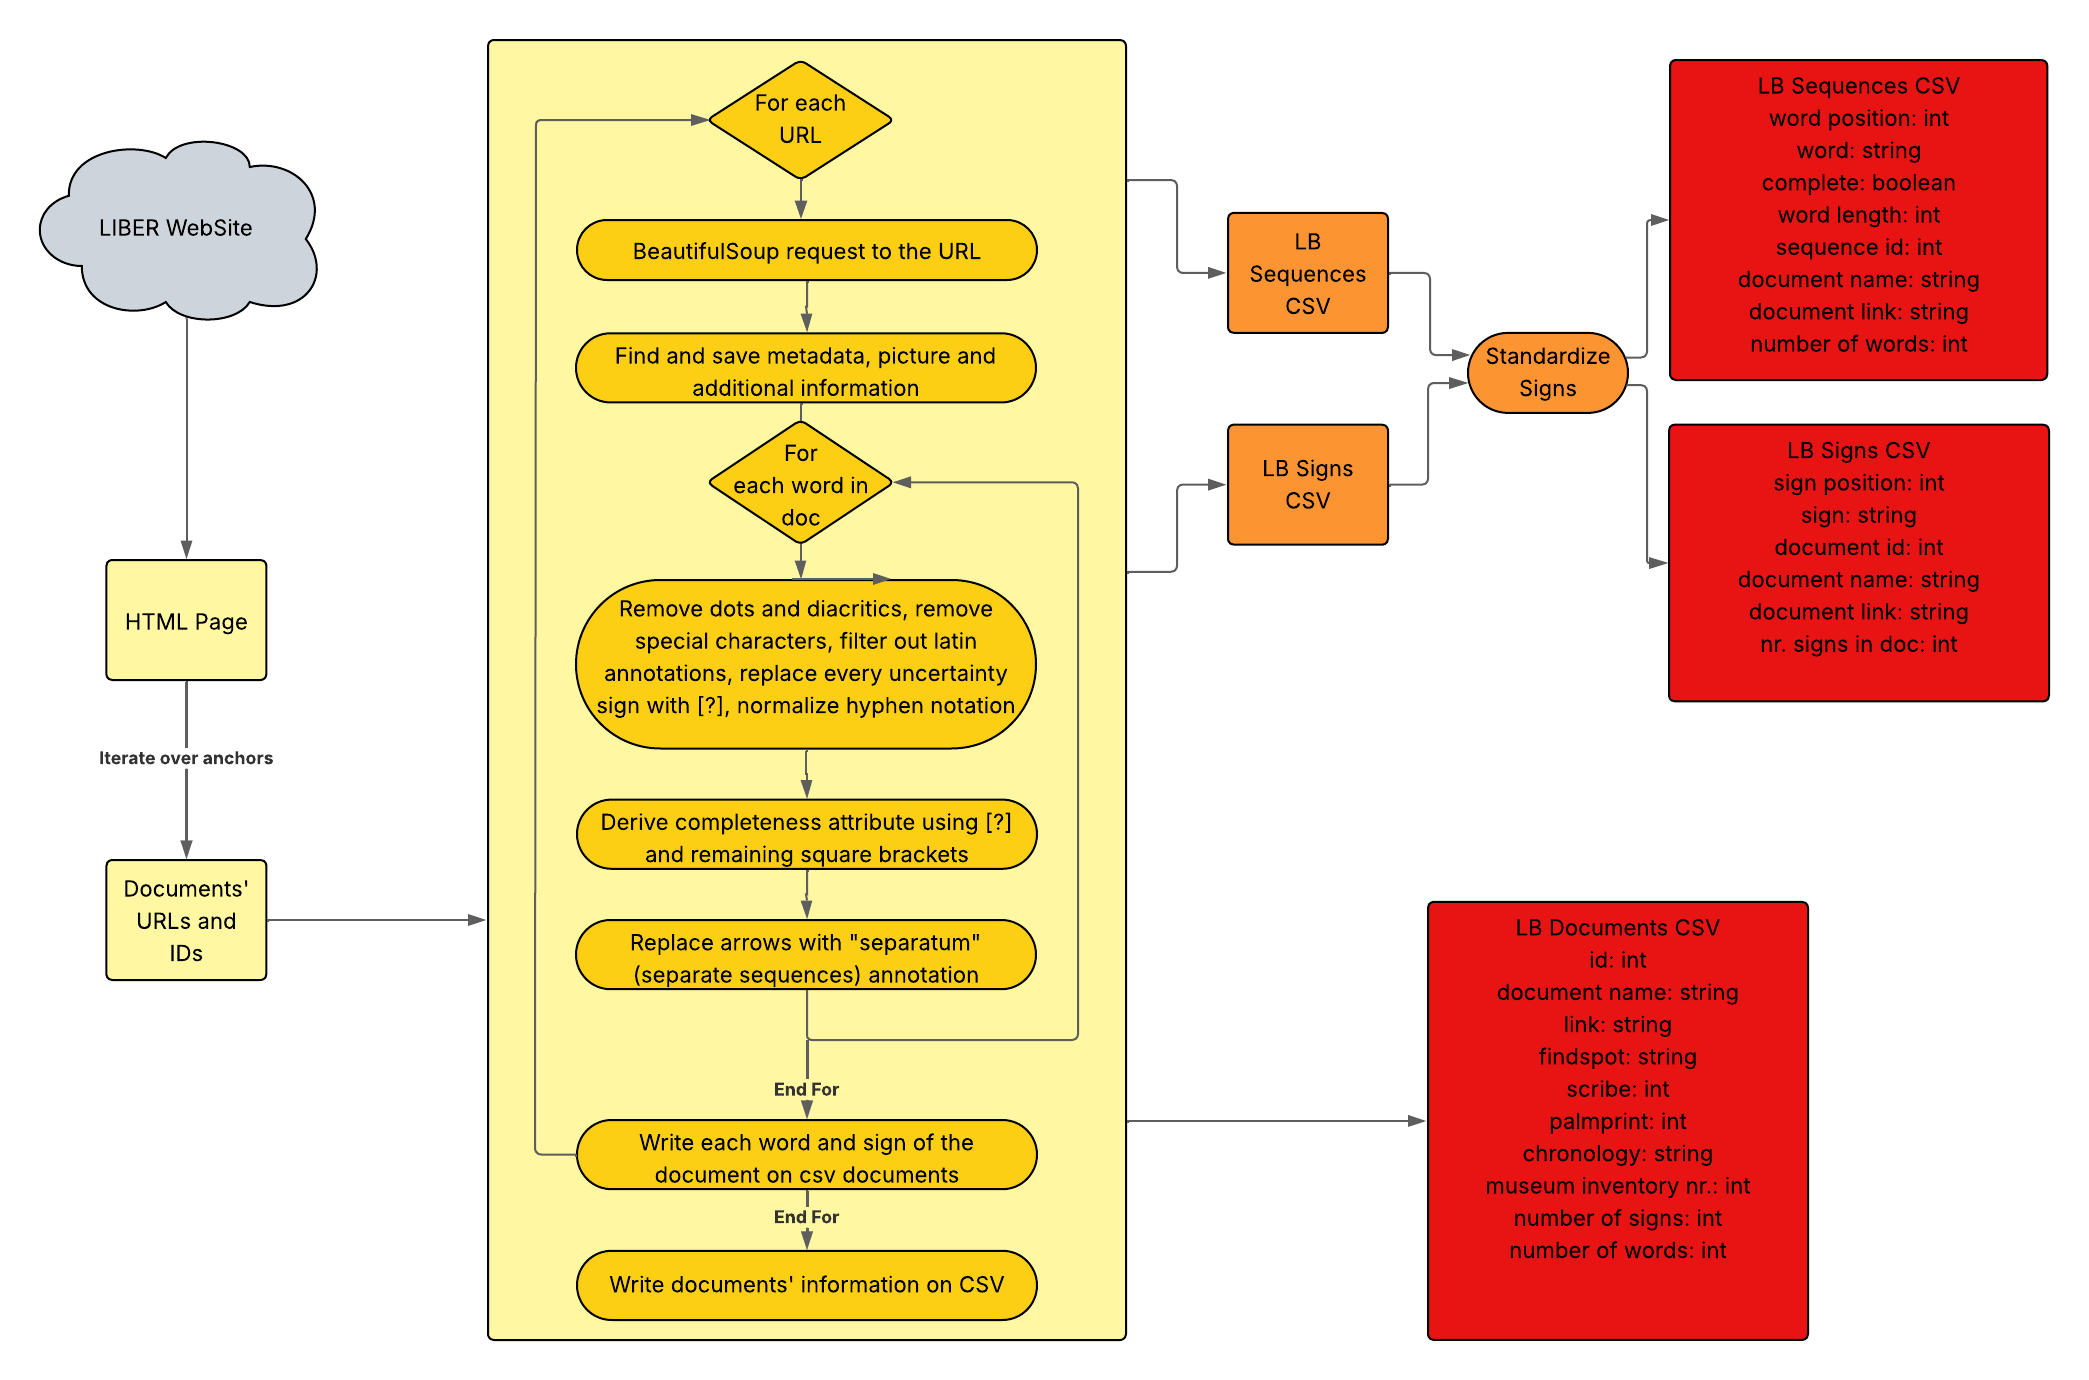
\includegraphics[width=1.1\textwidth]{images/webscrape_linb.png}
    \end{adjustbox}
    \caption{Webscraping and processing of Linear B data from the LiBER archive.}
    \label{fig:webscrape-lb}
\end{figure}

\subsection{Ancient Greek}
For Ancient Greek we required a broad lexicon, preferably skewed toward earlier forms that preserve Mycenaean reflexes more than later Classical usage.
To that end, the Homeric epics (the Iliad and the Odyssey) were collected and preprocessed to a normalized orthography, described in Section \ref{sec:datasets}.

The resulting high-coverage type list serves the brute-force cognate matching stage (Section \ref{sec:bruteforce-cognates}), where the entire Linear B corpus is compared against normalized Homeric forms to surface plausible cognate candidates.

\section{Related Work}
The work presented in this thesis builds upon and extends prior research in historical linguistics, computational decipherment, and natural language processing.

For the historical and linguistic background of Aegean scripts, I relied on foundational texts, such as Minoan Civilization by Spyros Alexiou \cite{alexiou-ch2}, Aegean Linear Script(s) by Ester Salgarella \cite{salg-ch1}, and The Decipherment of Linear B by John Chadwick \cite{chad-ch2}.

In the realm of computational decipherment, the most relevant prior work consisted of contributions on the text infilling task by Katerina Papavassileiou \cite{brnn-paper} and the cognate matching task by Jiaming Luo \cite{luo}.  
Notably, in both cases the models used to encode Linear B sequences are based on bidirectional recurrent neural networks (BRNNs), which are also used in this work.  
For the text infilling task, I also assessed the effectiveness of transformer-based architectures, noting a significant drop in performance compared to RNNs, mostly due to the scarcity of training data. 

Lastly, the prompt-engineering approach to translation and reconstruction is inspired by the advantages of large language models (LLMs) and their demonstrated ability to understand and translate Ancient Greek.  
By supplying the information that is strictly necessary for translation and reconstruction, the Linear B corpus can be automatically translated into English.

\subsection{Cognate Matching and Manual Decipherment}
Cognate matching has been used in several prior works to support the decipherment of ancient scripts.  
Ventris and Chadwick themselves relied on simple cognate identification at the start of their decipherment of Linear B.  
Automating cognate detection is a crucial step toward scaling decipherment efforts to larger corpora and more complex scripts.  
Luo proposed a language-agnostic neural model for cognate matching, which I tested and extended in this thesis (Section \ref{sec:generative-framework}).

The models’ output was used to generate a list of candidate cognate pairs, which were provided as input to an LLM.  
Alongside these, I supplied additional linguistic information useful for grammatical, logical, and syntactical analysis.  
The LLM was then prompted to produce an Ancient Greek reconstruction and translate it into English, using structured processing instructions, typical of manual decipherment, and a few examples.  
The steps of this process are described in detail in Section \ref{sec:final-prompt}.


\chapter{The Aegean Linear Scripts}
Linear A and Linear B were writing systems used during the Bronze Age, primarily on the island of Crete, with some discoveries also made on the Greek mainland.

\section{Historical Context}
Around 2000 BCE, the already established Minoan civilization on the island of Crete began constructing large, complex architectural buildings commonly referred to as "palaces."
These edifices served not only as administrative and economic centers, but also played important religious and ceremonial roles within Minoan society.

The founders of these palatial complexes were undoubtedly powerful landowners.
Minoan society was highly organized and capable of mobilizing substantial manpower for major construction projects, such as leveling the hilltops at Knossos and Phaistos and erecting monumental palaces. \cite{alexiou-ch2}

Hence, this highly structured society began to feel the need for a form of administrative writing to record transactions, compile inventories, and manage other aspects of economic and bureaucratic activity.

The first form of writing developed by this society was a logographic script known as Minoan Hieroglyphics, or Cretan Hieroglyphics, attested between 2100 and 1700 BCE.
The earliest and most archaic script was composed entirely of logographic symbols, which superficially resembled Egyptian hieroglyphs.
It was later abandoned in favor of a linear script known as Linear A, employed between 1800 and 1450 BCE.
The two systems initially coexisted for over a century, but in the following years, Linear A gradually replaced the former and became the sole writing system in use. \cite{salg-ch1}

Notably, the latest attestations of Cretan Hieroglyphs date to around 1700 BCE, when a catastrophe struck the island of Crete.
All the palaces in the island's three main centers, Knossos, Phaistos, and Malia were destroyed.
However, this did not lead to a cultural shift, as the palaces were promptly rebuilt, marking the passage from the Proto-palatial to the Neo-Palatial phase in Minoan history. \cite{alexiou-ch3}

This second phase of palace construction is the one that has survived to the present day, particularly at sites such as Knossos, Phaistos, Malia, and Zakros.

In 1450 BCE, a major catastrophe struck, probably caused by the eruption of the Thera volcano.
It triggered devastating earthquakes and a tidal wave that swept the north coast of Crete.
As a result, the main centers of Minoan civilization, Phaistos, Aghia Triadha, Malia, the mansions of Tylissos and Ammisos, as well as the eastern cities of Gournia and Zakros, were reduced to ruins.
Knossos also suffered significant damage, often accompanied by widespread fires. \cite{alexiou-ch4}

In 1400 BCE, Crete began losing its central cultural role, and the focus shifted to mainland Greece, particularly the Peloponnese.
The palace of Knossos was destroyed, while major fortified citadels (fortresses) were built in places like Mycenae and Tiryns. \cite{alexiou-ch5}

During this period, a new linear writing system emerged.
Although visually similar to Linear A, it encoded a different language: an archaic form of Ancient Greek.
Its name is Linear B, and it was used from 1400 to around 1100 BCE on Crete and the Greek mainland.
The Mycenaean civilization, which flourished during this period, is characterized by its extensive use of Linear B for administrative purposes, particularly in palace economies.
However, the destruction in Crete should not be interpreted as a Mycenaean military takeover, but rather as a transformative phase of socio-political and cultural adaptation. \cite{salg-ch5}


\begin{table}[h!]
\centering
\caption{Chronological framework of LA and LB \cite{salg-ch1}}

\begingroup
\renewcommand{\arraystretch}{0.9}
\resizebox{\textwidth}{!}{%
\begin{tabular}{|c|c|c|c|c|c|c|}
\hline
\multicolumn{1}{|c|}{\textbf{Chronology}} & \multicolumn{3}{c|}{\textbf{Crete}} & \multicolumn{3}{c|}{\textbf{Mainland}} \\
\hline
\textbf{High Dating} & \textbf{Pottery Phase} & \textbf{Cultural Phase} & \textbf{Scripts} & \textbf{Pottery Phase} & \textbf{Cultural Phase} & \textbf{Scripts} \\
\hline
1900--1800 & MM II      & \multirow{2}{*}{Proto-Palatial} & CH; LA & MH III   & \multirow{2}{*}{--}               &  -- \\
1800--1700 & MM III     &                                & CH; LA & MH III   &                                 &  -- \\
\hline
1700--1600 & LM IA      & \multirow{2}{*}{Neo-Palatial}   & LA     & LH I     & \multirow{3}{*}{Early Mycenaean} & LA \\
1600--1450 & LM IB      &                                 & LA     & LH IIA   &                                 & ? \\
\cline{1-4}
1450--1400 & LM II      & \multirow{2}{*}{Final-Palatial} & LA?    & LH IIB   &                                 & ? \\
\cline{5-7}
1400--1375 & LM IIIA1   &                                 & LB     & LH IIIA1 & \multirow{4}{*}{Late Mycenaean}  & LB \\
\cline{1-4}
1375--1300 & LM IIIA2   & \multirow{3}{*}{Post-Palatial}  & LB     & LH IIIA2 &                                 & LB \\
 % separate lines for Crete and Mainland
1300--1200 & LM IIIB    &                                 & LB     & LH IIIB  &                                 & LB \\
% separate lines for Crete and Mainland
1200--1050 & LM IIIC    &                                 & --     & LH IIIC  &                                 & LB \\
\hline
\end{tabular}
}
\endgroup
\end{table}


\section{The main sites}
The main sites where Linear A documents have been found are located on the island of Crete. These include Knossos, Phaistos, Aghia Triada, Zakros, Khania, Tylissos, and Malia.

\begin{figure}[H]
    \centering
    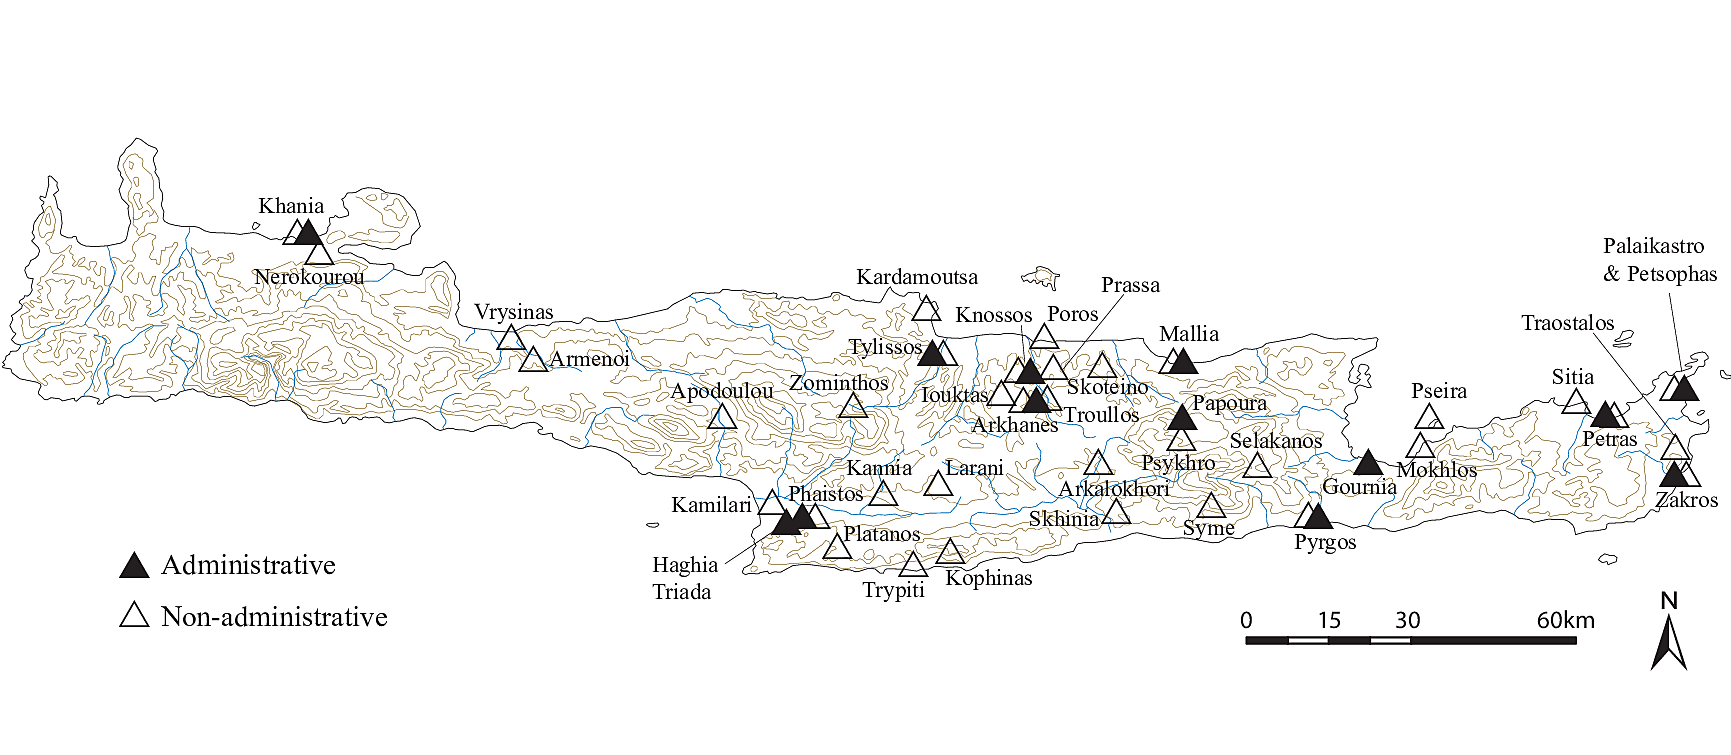
\includegraphics[width=0.8\textwidth]{Images/crete_LA.png} % Adjust width and filename
    \caption{Sites of Linear A fragments in Crete.\protect\footnotemark}
    \label{fig:crete_LA}
\end{figure}
\footnotetext{Figure \ref{fig:crete_LA} prepared by Yannis Galanakis and Ester Salgarella.}

Linear A was more widespread, covering completely Crete and the Aegean Islands and reaching the Greek mainland.
The main attestations of Linear A on the Greek mainland are very limited and generally considered sporadic and isolated. 
At Mycenae, a few Linear A inscriptions have been found, likely as a result of commercial or cultural exchanges with Crete. 
Similarly, some fragmentary finds have been uncovered at Tiryns, probably also related to trade or contacts with Minoan Crete.

\begin{figure}[H]
    \centering
    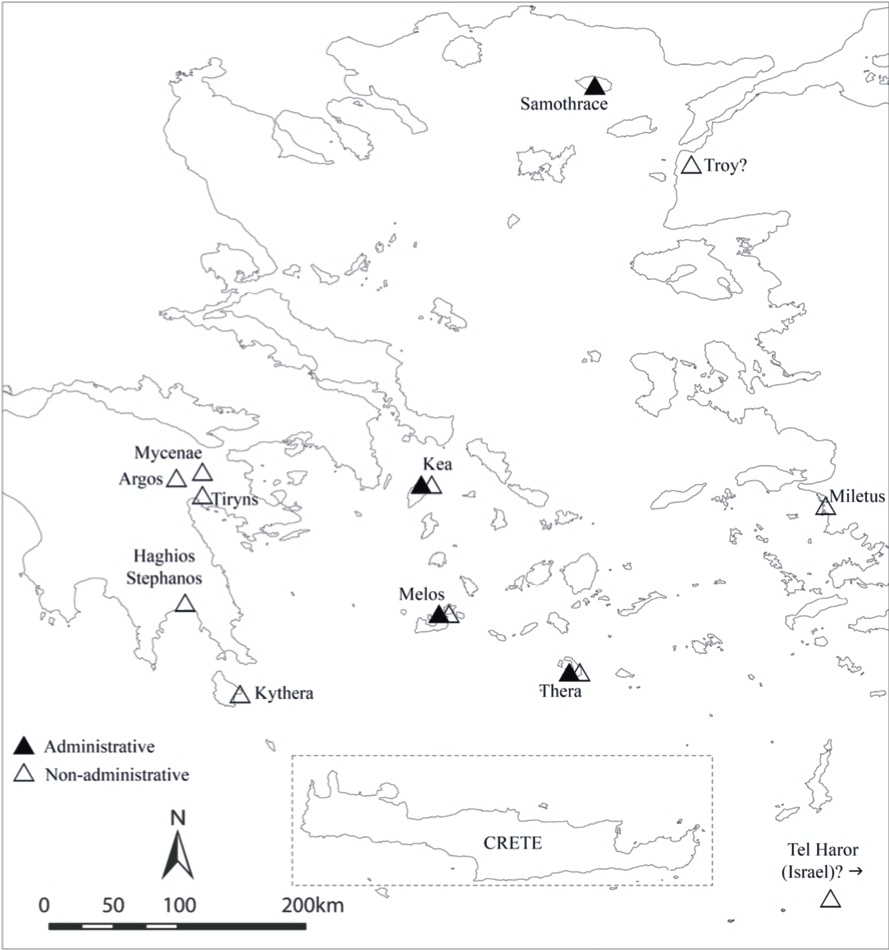
\includegraphics[width=0.8\textwidth]{Images/mainland_LA.jpg} % Adjust width and filename
    \caption{Sites of Linear A fragments in the Greek mainland.\protect\footnotemark}
    \label{fig:mainland_LA}
\end{figure}
\footnotetext{Figure \ref{fig:mainland_LA} prepared by Yannis Galanakis and Ester Salgarella.}

In contrast, Linear B is extensively attested on the Greek mainland, particularly in the Peloponnese, reflecting its administrative function during the Mycenaean period.
Major sites where Linear B documents have been found include Mycenae, Tiryns, Pylos, Thebes, and Athens.
Additionally, significant findings of Linear B tablets have been made in Crete, especially at Knossos and Khania.

The corpora of the two writing systems are relatively small, with Linear A consisting of approximately 1,400 documents, while Linear B comprises around 6,000 documents.
Another notable difference is that Linear A was more widely used for non-administrative purposes, particularly in religious contexts, whereas the number of non-administrative Linear B documents is considerably more limited. \cite{salg-ch1}


\begin{figure}[H]
    \centering
    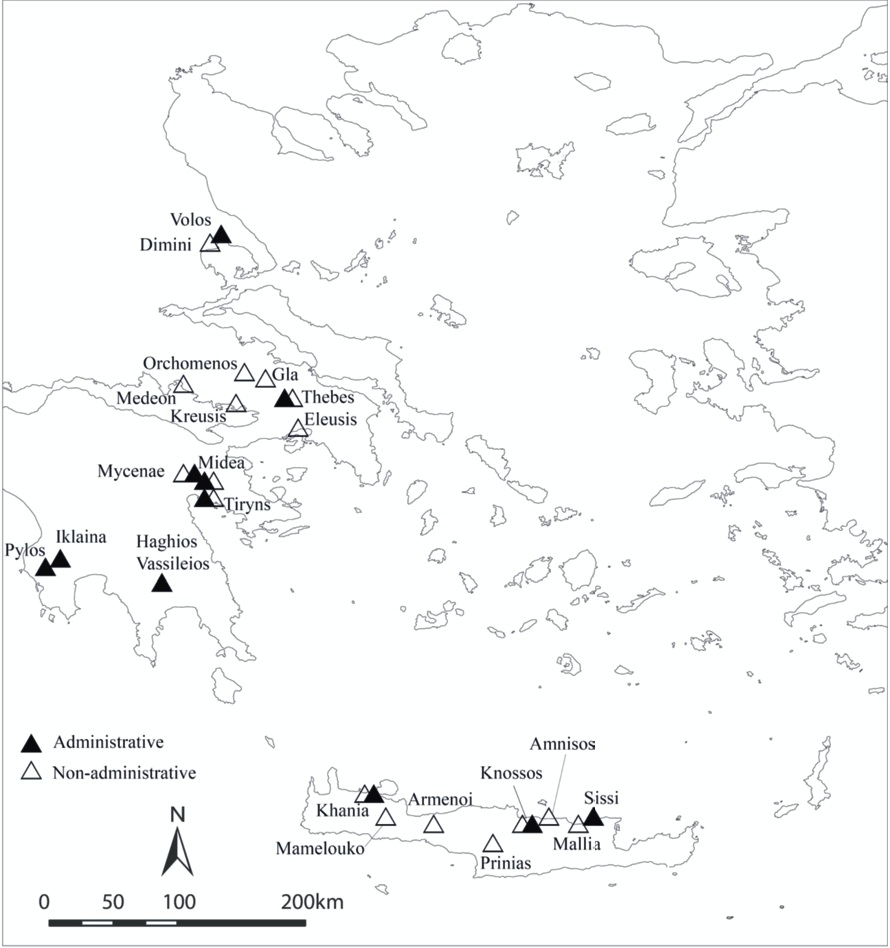
\includegraphics[width=0.8\textwidth]{Images/mainland_LB.jpg} % Adjust width and filename
    \caption{Sites of Linear B fragments in Crete and the Greek mainland.\protect\footnotemark}
    \label{fig:mainland_LB}
\end{figure}
\footnotetext{Figure \ref{fig:mainland_LB} prepared by Yannis Galanakis and Ester Salgarella.}


\section{Linguistic features}
The two writing systems are characterized by similar structural features, reflecting the connection between Linear A and Linear B and the derivation of the latter from the former.

The primary similarity between the two scripts lies in their syllabic structure, which constitutes a defining feature of both writing systems.
Both Linear A and Linear B are syllabic scripts, meaning that each symbol represents a syllable rather than an individual letter or a full word.
In addition to syllabic signs, both systems incorporate a set of logograms: symbols representing entire words or concepts.

This logographic component is particularly prominent in Linear A, where a significant number of signs are used to denote specific objects, actions, or concepts, often associated with administrative and religious contexts.
By contrast, Linear B employs a more restricted set of logograms, reflecting its primary function in administrative record-keeping.
Notably, the logograms used in Linear A were generally not inherited by Linear B, with a single exception: the logogram for "wool" (MA+RU), which is attested in both scripts.
However, the principles governing the formation of logograms remained unchanged, as in both scripts they are formed by juxtaposing or combining two or more signs, either horizontally or vertically.
\begin{figure}[H]
    \centering
    \begin{subfigure}[b]{0.6\textwidth}
        \centering
        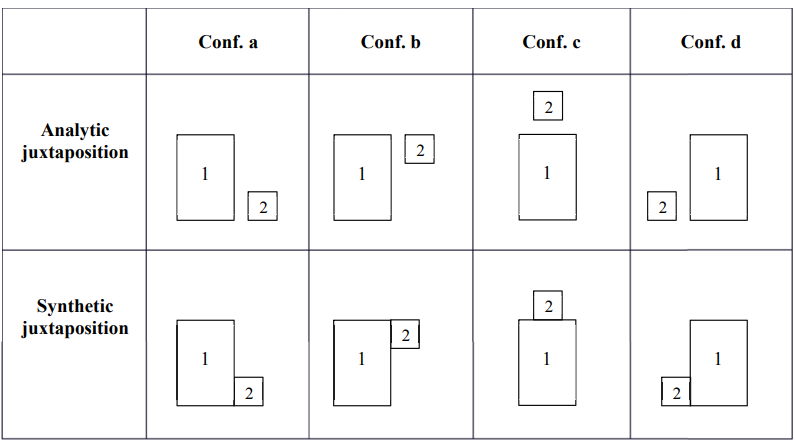
\includegraphics[width=\textwidth]{Images/logograms.png}
        \caption{Logogram construction criteria.}
        \label{fig:logograms}
    \end{subfigure}
    \hspace{0.05\textwidth}
    \begin{subfigure}[b]{0.3\textwidth}
        \centering
        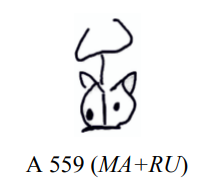
\includegraphics[width=\textwidth]{Images/ma-ru.png}
        \caption{LA logogram for wool.}
        \label{fig:ma-ru}
    \end{subfigure}
    \caption{Logograms in Linear A and Linear B.}
    \label{fig:linearA_sites}
\end{figure}

\begin{figure}[H]
    \centering
    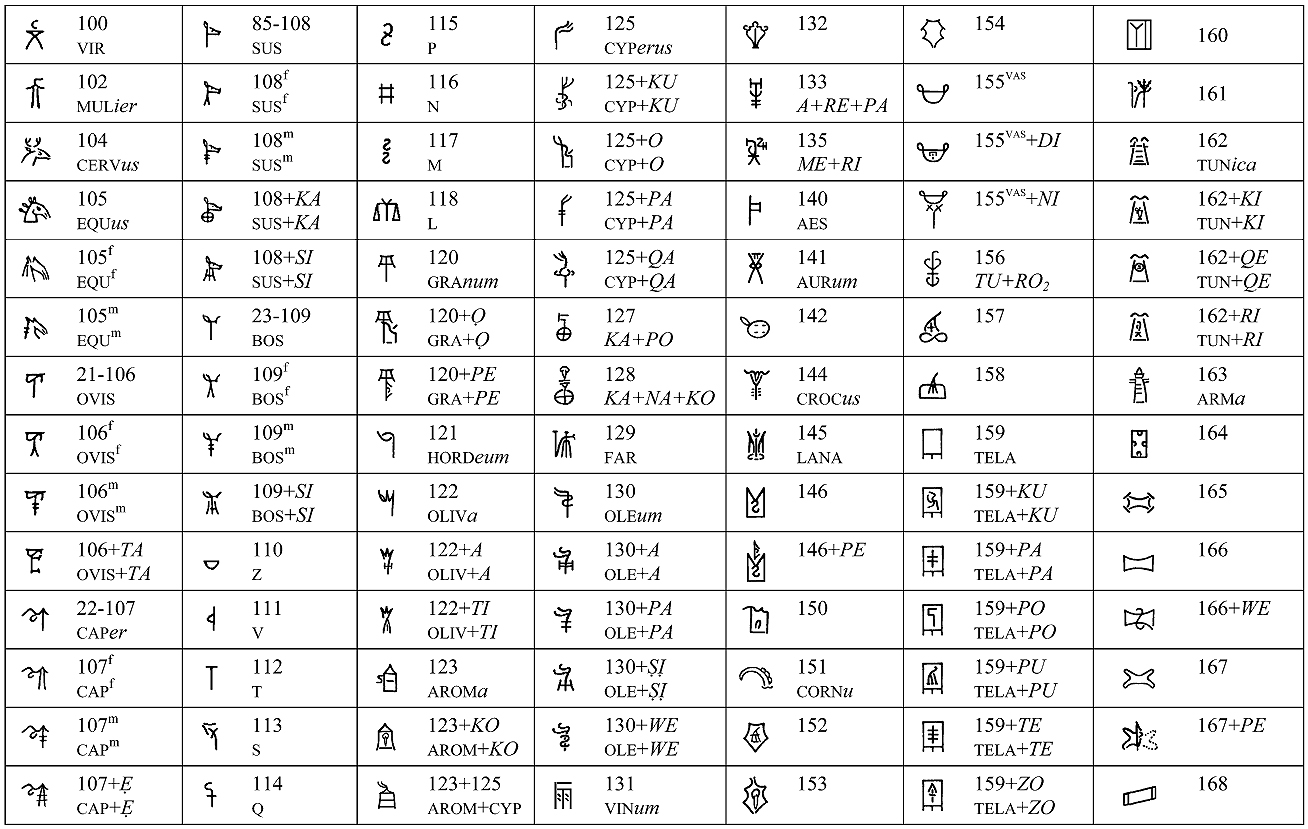
\includegraphics[width=1\textwidth]{Images/logos_1.jpg}
    \caption{Linear B logograms (symbols 100-168).}
    \label{fig:logos_1}
\end{figure}

Figure \ref{fig:logos_1} illustrates how logograms in Linear B can also incorporate syllabograms.
In these cases, the syllabogram is referred to as an adjunct and typically serves to qualify or specify the meaning of the logogram.
Moreover, the use of adjuncts is significantly more frequent in the Knossos corpus than on the Mainland, suggesting a possible continuity with Linear A, where isolated signs with sematographic value appear more commonly. \cite{salg-ch3}

Furthermore, a substantial portion of the Linear A syllabary is shared with Linear B, with approximately 72\% of Linear A signs being identical to those used in Linear B.
This overlap also illustrates continuity in symbol creation and in the assignment of phonetic values between the two systems.

\begin{figure}[H]
\centering
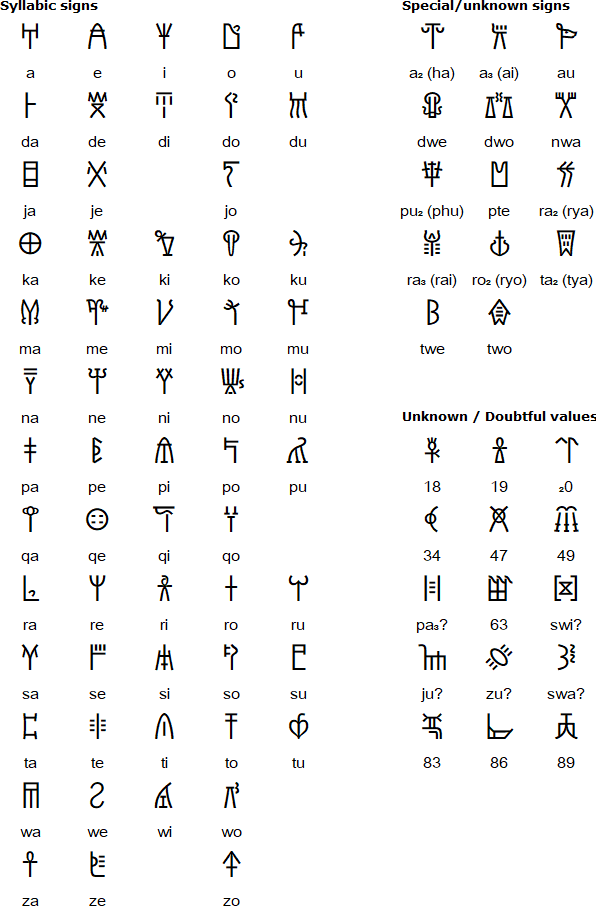
\includegraphics[width=0.8\textwidth]{Images/syll_LB.png}
\caption{All Linear B syllabograms with the associated phonetic values.}
\label{fig:syll_LB}
\end{figure}

As observed in Figure \ref{fig:syll_LB}, signs referring to the same vowel exhibit recurring patterns, a characteristic feature of syllabic scripts also evident in Linear A.
One of the most debated assumptions regarding the relationship between Linear A and Linear B is the principle of homomorphy and homophony.
This principle posits that signs which are visually similar (homomorphy) in both scripts also share the same phonetic value (homophony), representing the same syllable. \cite{salg-ch1}

This observation has led to the widely accepted conclusion that Linear A encodes a language fundamentally different from Linear B, with the latter used to represent an archaic form of Ancient Greek.
Consequently, although scholars are able to phonetically transcribe Linear A inscriptions, the language remains undeciphered and its meaning unknown. 

\section{The decipherment of Linear B} \label{sec:decipherment}
Ever since the discovery of the first Linear B tablets in 1900 by Sir Arthur Evans at Knossos, the script has been a subject of intense scholarly interest.
Evans himself introduced the classification of Aegean scripts that is still used today.
He also made the earliest attempts to decipher Linear B, though without success.

The breakthrough in understanding Linear B came after World War II, following major discoveries at the site of Pylos in 1939, which uncovered a large number of tablets and inscriptions.
A key figure in the decipherment of Linear B was Michael Ventris, a British architect and amateur linguist.
Ventris, in collaboration with philologist John Chadwick, succeeded in deciphering the script in 1952, demonstrating that it encoded an early form of Ancient Greek.

\subsection{The knowledge before the decipherment}

Before the decipherment of Linear B, scholars attempted to understand the script by studying it in isolation and by comparing it with known languages.  
One of the earliest hypotheses focused on the similarity between the Linear B syllabary and the Cypriot syllabary, a syllabic script used from about the eleventh to the fourth centuries BCE.  
The latter, which was also used to write an archaic form of Greek, shared a significant number of signs with Linear B.

However, this resemblance proved misleading in several respects.  
Although many signs appeared visually similar, as can be observed in Figure \ref{fig:lb-cypr}, their phonetic values often differed between the two systems.  
Moreover, the scripts treated grammatical suffixes differently.  
In Linear B, grammatical suffixes were frequently omitted, whereas this was not the case in the Cypriot syllabary, where the syllabogram "se" was regularly employed to indicate word endings.

Because "se" appeared regularly in the Cypriot syllabary but was rare in Linear B, early researchers concluded that Linear B could not represent the Greek language.  
In particular, Arthur Evans was convinced that the Minoan civilization was entirely distinct from the Mycenaean Greek world.  
This assumption, reinforced by Evans's authority and influence, contributed to delaying the recognition of the script's true linguistic nature. \cite{chad-ch2}

An example of this is the word "anthropos" (Ancient Greek: \textgreek{ἄνθρωπος}), which appears in Linear B as "a-to-ro-qo" (\textlinb{\Ba\Bto\Bro\Bqo}), while in Cypriot it is spelled with the "se" suffix as follows: "a-to-ro-po-se" (\textcypr{\Cse\Cpo\Cro\Cto\Ca}, written from right to left).

\begin{figure}[H]
\centering
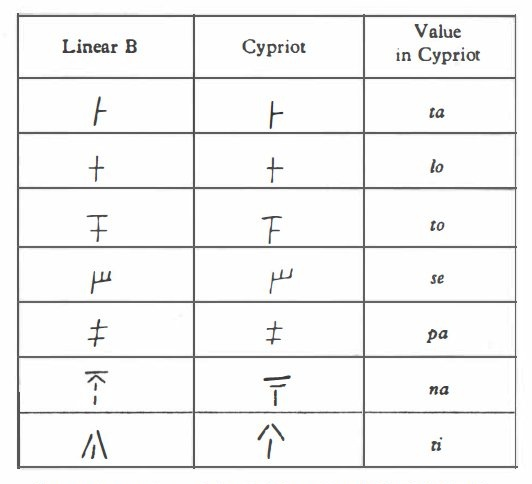
\includegraphics[width=0.6\textwidth]{Images/LB_cypriot.jpg}
\caption{Similarity between Linear B and Cypriot syllabary.}
\label{fig:lb-cypr}
\end{figure}

Evans had already established that most documents were administrative records.  
However, any attempt to decipher the script was hindered by unreliable underlying assumptions, while many aspects of the language remained unknown.

The most significant contribution came from Dr. Alice Kober, an American linguist. 
She was the first to approach the script methodically in order to uncover the nature of the underlying language.
She sought to answer fundamental questions, such as whether the language was inflected or whether specific forms were used to indicate gender and number.

Through her careful analysis, she was able to identify grammatical patterns, including distinctions between masculine and feminine nouns, as well as examples of inflection.
These results were achieved through a systematic study of repeated sign groups and their contexts, which she meticulously documented in her notebooks.
Her work challenged Evans's assumptions about the non-Greek nature of the language and paved the way for Ventris' later decipherment.
The outcome of her research was a set of "triplets", groups of three related words differing only in their endings, which provided critical evidence of an inflected language structure and were later referred to as "Kober's triplets".
Some examples of these triplets are shown in Figure \ref{fig:kobler_triplets}. \cite{chad-ch3}


\begin{figure}[H]
\centering
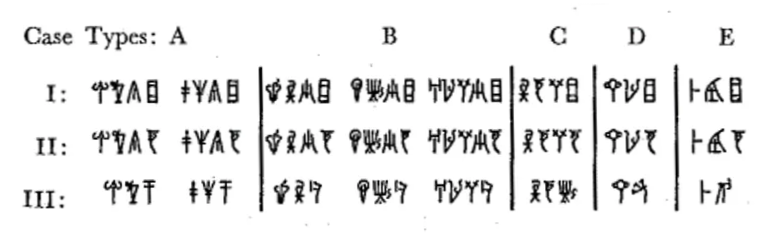
\includegraphics[width=0.8\textwidth]{Images/kobler_triplets.png}
\caption{Kobler's triplets examples.}
\label{fig:kobler_triplets}
\end{figure}

\subsection{The decipherment by Ventris and Chadwick} \label{subsec:ventris-chadwick}
The initial phase of the decipherment of Linear B involved the identification of numerical signs and easily recognizable logograms.
This preliminary work was largely accomplished by Sir Arthur Evans, who successfully identified the most frequently occurring logograms and reconstructed the basic features of the numerical system.
Notably, the Linear B script lacked a symbol for zero, but included fractional signs and was based on a decimal structure.

Building on these foundations, scholars began to assign tentative phonetic values to individual syllabograms through contextual analysis.
By examining recurring patterns and the placement of signs within administrative texts, it became possible to propose the phonetic values of certain symbols.
For instance, words such as "total" and "sons," which regularly appeared in similar tabular contexts, offered valuable clues for these early phonetic assignments.

However, the construction of a comprehensive and reliable grid of syllabograms was not feasible until the publication of the Pylos tablets in 1951.
This newly available corpus significantly expanded the body of evidence, enabling more systematic linguistic analysis.

Michael Ventris began his work on the decipherment in 1950, initially by circulating a questionnaire among scholars to gather views on the possible nature of the language encoded in Linear B and its potential relationship to Linear A or the Cypriot syllabary.

Realizing that scholarly opinion was divided, Ventris adopted a combinatorial and structural approach.
He explored positional patterns of signs within words, aiming to deduce their possible function or phonetic value.
By analyzing the frequency and distribution of certain symbols, particularly those likely to represent vowels, he was able to identify a subset of syllabograms corresponding to pure vowels.

A key breakthrough came from the identification of inflectional endings, many of which were made possible by the foundational work of Alice Kober.
Kober had demonstrated, through rigorous tabulation of sign groups, that the language encoded by Linear B exhibited an inflectional structure.
Ventris incorporated these findings into his research and began constructing a syllabic grid, updating it continually in light of new phonological rules and morphological patterns.

For example, he correctly identified the syllabogram \textlinb{\Bsi} as representing the syllable si, based on its frequent use in noun declensions and verb conjugations.
Its function mirrored that of the Ancient Greek suffix \textgreek{σι}, which appears in both oblique noun forms and verbal endings.

Additionally, place names proved particularly helpful, especially when accompanied by adjectival derivatives.
These offered valuable comparisons with known Greek toponyms and morphological structures.

As Ventris refined his hypotheses and incorporated increasingly sophisticated linguistic deductions, especially regarding inflectional patterns and suffixes, he was able to assign phonetic values to a majority of the signs.
Through this methodical approach, he successfully constructed a nearly complete syllabary grid.
Most of his assignments proved to be correct, with only minor exceptions that were later adjusted through collaborative efforts with John Chadwick and subsequent scholarly review. \cite{chad-ch4}

\begin{figure}[H]
\centering
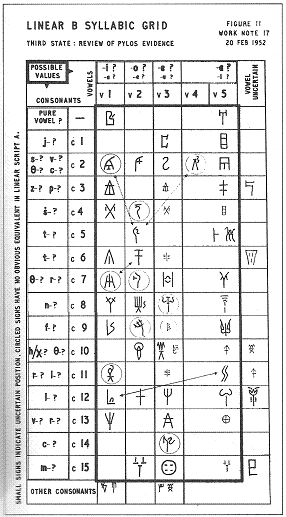
\includegraphics[width=0.8\textwidth]{Images/ventris_grid.png}
\caption{Ventris' syllabary grid.}
\label{fig:ventris_grid}
\end{figure}

Together, Ventris and Chadwick continued to investigate how the script encoded the phonology of the Mycenaean Greek language, recognizing that Linear B imposed structural constraints on how sounds were represented.
The syllabary, like many early writing systems, lacked a one-to-one correspondence with spoken Greek.
To better understand these adaptations, they analyzed the principles governing the script's orthography, namely how Greek words were transcribed within the limitations of the Linear B system.

The following rules summarize the most significant phonological and orthographic conventions that Ventris and Chadwick identified in the course of their research:

\begin{enumerate}
\item The script distinguishes five vowels: \textit{a, e, i, o, u}. Vowel length, however, is not indicated.

\item The second component of diphthongs ending in \textit{-u}, such as \textit{au, eu, ou}, is represented explicitly.

\item In diphthongs ending in \textit{-i} (e.g., \textit{ai, ei, oi, ui}), the second component is generally omitted, except:
\begin{itemize}
    \item when it occurs before another vowel, in which case it is represented as \textit{y};
    \item in the initial syllable \textit{ai}, where the full diphthong is retained.
\end{itemize}

\item Glides occurring between a front vowel and a following vowel are indicated:
\begin{itemize}
    \item the glide after \textit{i} is written as \textit{j};
    \item the glide after \textit{u} is written as \textit{w}.
\end{itemize}
These sounds are typically omitted in Greek alphabetic spelling.

\item The script represents twelve consonants:
\begin{itemize}
    \item \textbf{j}: used only to represent diphthongal \textit{i} or as a glide (see point 3);
    \item \textbf{w}: corresponding to the archaic Greek digamma (\textit{\textgreek{ϝ}}), pronounced as in English \textit{w};
    \item \textbf{d, m, n, s}: approximately as in later Greek and English;
    \item \textbf{r}: corresponding to Greek \textit{l} and \textit{r};
    \item \textbf{z}: corresponding to Greek \textit{z}; its exact phonetic value in Mycenaean Greek remains uncertain;
    \item \textbf{p, t, k}: representing both plain and aspirated stops, as the script does not distinguish aspiration;
    \item \textbf{q}: representing a series of labio-velar stops (\textit{kw, gw, khw}), which later disappeared from Greek but were preserved in Latin (e.g., \textit{quis}, \textit{unguem}).
\end{itemize}

\item The script does not represent aspiration; thus, aspirated consonants (\textit{ph, th, kh}) are not distinguished from their unaspirated counterparts.

\item The consonants \textit{l, m, n, r, s} are omitted when they occur:
\begin{itemize}
    \item at the end of a word;
    \item before another consonant.
\end{itemize}
For example, \textit{po-me} = \textit{poimen} (\textgreek{ποιμήν}) "shepherd"; \textit{ka-ko} = \textit{khalkos} (\textgreek{χαλκός}) "bronze"; \textit{pa-te} = \textit{pater} (\textgreek{πατήρ}) "father".

\item Initial \textit{s-} is generally omitted before another consonant.

\item In consonant clusters involving a stop + \textit{w}, both consonants are represented, with an intervening vowel that is either taken from the following syllable or supplied as a default. However, \textit{r} preceding \textit{w} is typically omitted.

\item Stop consonants (\textit{d, k, p, q, t}) occurring before another consonant are typically written with the vowel of the following syllable (less often the preceding syllable). 
For example:
\begin{itemize}
    \item \textit{ku-ru-so} = \textit{khrusos} (\textgreek{χρυσός}) "gold";
    \item \textit{A-mi-ni-so} = \textit{Amnisos} (\textgreek{Ἀμνισός}).
\end{itemize}
Special orthographic solutions are used to represent final consonant clusters, as in:
\begin{itemize}
    \item \textit{wa-na-ka} = \textit{wanax} (\textgreek{ϝάναξ}) "king".
\end{itemize}
\end{enumerate}

These conventions reveal the extent to which the Linear B script adapted to the phonology of Mycenaean Greek, despite being constrained by a syllabic system originally designed for a different language. \cite{chad-ch5}

The decipherment of Linear B was finally confirmed one year later, when in 1953 a new tablet found in Pylos could be translated only by using Ventris' grid.
This independent verification of the decipherment on material not previously available to Ventris provided undeniable evidence of his success. \cite{chad-ch6}

The work of Ventris and Chadwick, by combining structural analysis with comparative linguistics, thus not only unlocked the meaning of Linear B but also illuminated the phonological landscape of the earliest attested form of the Greek language.
\chapter{The cognate matching task}
As explained in Section \ref{sec:decipherment}, the decipherment of Linear B required a collective effort that involved several scholars and extended over multiple decades.

The main difficulties in any decipherment process concerning ancient languages arise from two factors: the absence of parallel texts that could guide the interpretation, and the extreme scarcity of surviving documents.
Even for domain experts, decipherment therefore demands encyclopedic linguistic and historical knowledge, combined with an enormous amount of manual work that is often prohibitive in terms of time and resources.
Moreover, the challenges encountered during the decipherment of one language are rarely reusable for others, since much of the required work and insights are closely tied to the specific features of that language and cannot be easily generalized \cite{luo}.
For example, the rules mentioned at the end of Section \ref{subsec:ventris-chadwick} are highly specific to the context of Linear B and its unique characteristics, and do not even apply to closely related scripts, such as Cypriot or possibly Linear A (for which no certainty exists, as the language remains undeciphered).

For these reasons, the introduction of computational methods and machine learning techniques has the potential to provide crucial assistance.
Nevertheless, the central obstacle remains the limited amount of training data.
This scarcity of examples makes it essential to design models that are able to learn effectively from small datasets and to generalize from minimal evidence.

In this respect, it is important to note that not all machine learning architectures are equally suitable for such low-resource conditions.
Transformers, for example, are a class of neural networks that have achieved remarkable results in modern natural language processing tasks, such as machine translation and text generation.
However, their success is strongly dependent on access to very large training corpora.
In the absence of such data, as is the case for ancient scripts, the application of transformers becomes impractical.
This explains why alternative architectures, which are better suited to scenarios where training data is scarce, are currently preferred in the computational study of ancient languages.

\section{Identifying Cognates}
Cognates are words in different languages that share a common etymological origin.
Identifying cognates is a crucial task in historical linguistics, as it allows researchers to trace the evolution of languages and to understand their relationships.
In the case of Linear B, the identification of cognates provided valuable correspondences between the syllabic script and the phonetic representations of Ancient Greek, which proved instrumental in the decipherment process.
Cognate matching was indeed a key aspect of Ventris' work, as he relied on clearly identifiable cognates to assign phonetic values to Linear B signs.
However, the task of identifying cognates is not always straightforward, since it requires a deep understanding of the historical and linguistic context of the languages involved.
In addition, several phonological transformations had taken place over time, including the differentiation of aspirated consonants and the loss of certain sounds once present in Linear B, such as the digamma ({\textgreek{ϝ}}) and the labio-velar consonant \textit{q}.

Below are some examples of cognates identified between Linear B and Ancient Greek:  

\begin{itemize}  
    \item \textlinb{\Ba\Be\Bti\Bto} (a-e-ti-to) $\rightarrow$ \textgreek{ἀέθιστος}, \textgreek{ἐθίζω} \\  
    This example shows how a Linear B sequence corresponds directly to a recognizable Greek adjective and verb.

    \item \textlinb{\Ba\Bdi\Bnwa\Bta} (a-di-nwa-ta) $\rightarrow$ \textgreek{Ἀδινϝᾶτας} \\  
    An instance where the Linear B syllabogram "nwa" reflects the presence of the digamma.

    \item \textlinb{\Be\Bma\Baii} (e-ma-ha) $\rightarrow$ \textgreek{Ἑρμᾶς}, \textgreek{Ἑρμαῖ}, \textgreek{Ἑρμαίας} \\  
    Illustrates a clear lexical link to Greek terms related to Hermes.

    \item \textlinb{\Bko\Bno\Bso} (ko-no-so) $\rightarrow$ \textgreek{Κνωσός}\\  
    A straightforward toponym, the name of the main Minoan palace site.

    \item \textlinb{\Bwo\Bno\Bqe\Bwa} (wo-no-qe-wa) $\rightarrow$ \textgreek{Φονοκέϝας}, \textgreek{Φονοκέϝαν} \\  
    Preserves traces of the digamma and labio-velar consonants.

    \item \textlinb{\Bwo\Bro\Bki\Bjo\Bne\Bjo} (wo-ro-ki-jo-ne-jo) $\rightarrow$ \textgreek{ϝοργιονείον}, \textgreek{Ὀργιονεῖος}, \textgreek{Ὀργίωνες} \\  
    A more complex example, relating to anthroponyms and associations.

    \item \textlinb{\Bqi\Bsi\Bpe\Be} (qi-si-pe-e) $\rightarrow$ \textgreek{ξίφεις}, \textgreek{ξίφη}, \textgreek{ξίφεα} \\  
    Reflects the Linear B representation of the Greek word for "sword."  

    \item \textlinb{\Bre\Bu\Bko\Bto\Bro} (re-u-ko-to-ro) $\rightarrow$ \textgreek{Λεῦκτρον}, \textgreek{Λεῦκτροι} \\  
    A toponym, attested both in Linear B and later Greek sources.

    \item \textlinb{\Bqo\Bu\Bqo\Bta} (qo-u-qo-ta) $\rightarrow$ \textgreek{Βουβώτας} \\  
    Demonstrates the phonetic evolution of labio-velar sounds.

    \item \textlinb{\Bqe\Bqi\Bno\Bme\Bna} (qe-qi-no-me-na) $\rightarrow$ \textgreek{γεγινώμενα}, \textgreek{γιγνόμενα} \\  
    A verbal form that shows continuity in Greek morphology.

    \item \textlinb{\Bpo\Bro\Bwi\Bto\Bjo} (po-ro-wi-to-jo) $\rightarrow$ \textgreek{πλωϝιστοῖο} \\  
    Example of a genitive form with preservation of the digamma.

    \item \textlinb{\Bpo\Bti\Bpi} (po-ti-pi) $\rightarrow$ \textgreek{Πόρτις}, \textgreek{Πόρτιφι} \\  
    Reflects a proper name with different Greek attestations.

    \item \textlinb{\Ba\Bri\Bqa} (a-ri-qa) $\rightarrow$ \textgreek{Ἄρισβας} \\  
    Example of an anthroponym preserving older consonantal values.

    \item \textlinb{\Bko\Bno} (ko-no) $\rightarrow$ \textgreek{Σκοῖνος} \\  
    Shows the addition of a consonant in Ancient Greek.
\end{itemize}  

\section{Datasets} \label{sec:datasets}
In this section, the process of gathering and preparing the datasets used in this study is described.
It is worth noting that I made several choices in order to create a clean and consistent dataset.
The main choices are the following:

\begin{itemize}
    \item All diacritics, accents, breathings, and iota subscripts were removed from Ancient Greek forms, resulting in a simplified text. For example \textgreek{ἀέθιστος} is represented as \textgreek{αεθιστος}.

    \item All instances of uppercase letters were converted to lowercase in order to normalize the data. For instance \textgreek{Κνωσός} is represented as \textgreek{κνωσος}.
    Note also that Linear B does not distinguish uppercase and lowercase.
    
    \item All instances of punctuation were removed.
    
    \item Linear B words were represented using their Latinized transcription.
    Therefore, the dataset contains the word \textlinb{\Bko\Bwo} as ko-wo instead of the original Linear B characters.

    \item The instances of digamma were inserted in a suitable position also in the Greek form, despite their disappearance from Classical Greek.
    For example, the word \textgreek{κόρος} is represented as \textgreek{κορfος} in the dataset.
    In some cases, the version without digamma is also included, as in \textgreek{κουρος}.

    \item The only additional symbol employed, besides the standard Greek alphabet, is "h", used to represent the aspiration conveyed by the syllabogram \textlinb{\Baii} (ha).
    For instance, \textlinb{\Ba\Bpi\Baii\Bro} (a-pi-ha-ro) is rendered as \textgreek{αμφιhαλος}.
\end{itemize}

The sources of all the data included in the final version of the dataset are the following:

\begin{itemize}
\item \textbf{Luo's dataset} \cite{luo}: a collection of cognates between Linear B and Ancient Greek, compiled by Jiaming Luo. It contains 919 Linear B words together with their proposed Ancient Greek correspondences.
\item \textbf{Chris Tselentis' *Linear B Lexicon*} \cite{tselentis}: a lexicon comprising 1338 Linear B entries with Ancient Greek equivalents. A substantial portion of these entries overlap with Luo's dataset.
\item \textbf{Ventris and Chadwick's Vocabulary} \cite{chadwick-notes}: a digitized compilation based on the original notes and lexical work of Michael Ventris and John Chadwick, later supplemented with commentary by other scholars. The resource, available as a CSV file at \url{https://linear-b.kinezika.com/lexicon.html}, comprises 2747 unique words.
It is organized as a vocabulary, offering definitions and interpretative remarks on the terms, and thus represents an extended digital derivative of their foundational work.
\end{itemize}

\subsection{Prompt engineering}
Some tasks were automated using prompt engineering techniques with Gemini~2.0~Flash and Gemini~2.5~Flash, which proved effective for text processing and data manipulation. Whenever these techniques are employed, I explicitly indicate their use and summarize the prompt instructions that were critical to the task.
In general, the prompts followed these principles:

\begin{itemize}
\item \textbf{Clarity and specificity:} Clear, unambiguous instructions to reduce variance and align outputs with task requirements \cite{prompting-programming}.

\item \textbf{Iterative refinement:} Prompts were refined based on model outputs to improve quality across iterations.

\item \textbf{Contextualization:} Task-relevant context (e.g., field definitions, examples) was included to guide disambiguation.

\item \textbf{Structured reasoning:} Prompts encouraged stepwise reasoning for complex tasks (e.g., breaking a problem into sub-steps), leading to more coherent outputs \cite{cot}.

\item \textbf{Structured formatting:} Outputs were requested in explicit schemas (XML/JSON, bullet/numbered lists) to ensure machine-readable, post-processable results.

\item \textbf{Salience cues (including UPPERCASE for emphasis):} Key requirements were emphasized to prioritize the most important aspects and reduce omission errors \cite{uppercase-is-all-you-need}.
\end{itemize}

When necessary, I adjusted the model's generation settings to favor determinism: the \texttt{temperature} was set low (e.g., 0.1--0.3) to reduce randomness and increase repeatability, and \texttt{top-k} was fixed at 1 (greedy selection).

\subsection{Luo's Dataset}
Luo's dataset is the one on which the creator of the NeuroDecipher model (introduced later) tested its performance.
The model achieves excellent results on this dataset, reaching an accuracy of 84.7\% of cognates correctly matched \cite{luo}.

However, the dataset is not without limitations.
The main issue I identified upon closer inspection is that some proposed Greek cognates are not attested in extant Ancient Greek sources, but rather tentative transliterations of Linear B forms or artificially modified versions of Greek correspondences.
While this may artificially improve the cognate matching task, it does not reflect a realistic linguistic scenario and makes the dataset unsuitable for use in an automatic translation pipeline.
A few illustrative examples are given below:

\begin{itemize}
\item \textlinb{\Bqo\Bo} (qo-o) is correctly associated with \textgreek{βους}, as also confirmed by Tselentis' lexicon \cite{tselentis}. However, the dataset additionally lists \textgreek{κfοος}, which does not correspond to any attested Ancient Greek form.
\item \textlinb{\Bto\Bo} (to-no) is linked to \textgreek{θρονος}, likewise confirmed by Tselentis' lexicon \cite{tselentis}, but the dataset also includes \textgreek{θορνος}, an unattested form that results from an unjustified inversion of letters.
This error extends to \textlinb{\Bto\Bro\Bno\Bwo\Bko} (to-ro-no-wo-ko), where the listed cognate is \textgreek{θορνοfοργος}. I corrected this instead to \textgreek{θρονοfοργος} and \textgreek{θρονοfεργος}, both plausible formations obtained by combining \textgreek{θρόνος} ("throne, chair") with the productive suffix derived from \textgreek{ἔργον} ("work, deed"). The resulting compound restores the original sense of the term as "chair-maker" or "craftsman of thrones."
\item In several cases, the dataset conflates distinct gendered forms by grouping them under a single entry. For example, \textlinb{\Bne\Bwa} (ne-wa), corresponding to \textgreek{νεfα} or \textgreek{νεα}, feminine, and \textlinb{\Bne\Bwo} (ne-wo), corresponding to \textgreek{νεfος} or \textgreek{νεος}, masculine, were all grouped under \textlinb{\Bne\Bwa}, despite both variants being independently attested in the Linear B corpus.
\end{itemize}

The adjustments described above were applied to Luo's dataset in order to enhance its reliability and linguistic accuracy.
This revised version was then used both to measure the performance of the NeuroDecipher model on a more realistic dataset and as the foundation for constructing the final comprehensive dataset, which also integrates additional material from Tselentis' Linear B Lexicon and from the digitized vocabulary of Ventris and Chadwick.
The resulting revised dataset comprises 976 Linear B entries paired with their respective Ancient Greek correspondences.

\subsection{Tselentis' Dataset}
Tselentis' dataset represents a valuable resource for the study of Linear B, as it comprises a comprehensive lexicon of Linear B terms and their corresponding Ancient Greek forms.
It serves as a crucial reference point for validating and enriching the cognate pairs identified in Luo's dataset.

The main drawback of Tselentis' lexicon is that it was only available as a PDF document, which made it necessary to manually transcribe the entries into a more usable format.
After using an online OCR tool to extract its content into a CSV file, followed by targeted cleaning, a structured file containing all the fields in the lexicon was obtained.

Nevertheless, the data still required further processing to extract the Greek and Linear B forms in accordance with the normalization criteria outlined at the start of this section.
Several parsing mistakes, along with inconsistencies in accents, diacritics, and formatting, had to be corrected to ensure accuracy and consistency.
To streamline this process, Prompt Engineering techniques were employed with Gemini~2.0~Flash, guided by explicit processing directives.

These techniques enabled the automated correction of recurrent errors and inconsistencies, significantly accelerating data preparation.
The processed dataset was then reviewed manually to ensure its quality and reliability before integration into the final comprehensive dataset.

For transparency and repeatability, I detail here the precise directives provided to Gemini for dataset processing.

\bigskip
\noindent\textbf{PROCESSING RULES FOR LINEAR B TO GREEK COGNATES:}

\begin{enumerate}[label=\textbf{\arabic*.}, leftmargin=2.5em]
\setcounter{enumi}{-1}

\item CRITICAL: DO NOT MAKE ANY MODIFICATION TO GREEK COGNATES OR LINEAR B SEQUENCES IF THE MODIFICATION IS NOT MENTIONED IN THE FOLLOWING RULES! DO NOT CHANGE THE INPUT IN ANY POSSIBLE WAY AND ONLY APPLY THE GIVEN MODIFICATION RULES! NO FANTASY JUST BLINDLY OBEY!

\item SPLITTING MULTIPLE WORDS: When Linear B field contains multiple words separated by "/", create separate JSON objects for each word, matching with the corresponding Greek cognate in the same position.

\item HANDLING PARENTHESES: For Linear B words with parenthetical elements like "po-ni-ke-(j)a", create two separate entries (one with and one without the parenthetical element, like "po-ni-ke-ja" and "po-ni-ke-a").

\begin{enumerate}[label*=\textbf{\arabic*.}, leftmargin=2em]
  \item HANDLING PARENTHESES FOR GREEK COGNATE: if a word is presented with optional greek characters with parenthetical elements like "\textgreek{αιξμά(ν)ς}", include both variants with and without the letter in parentheses.
  \item HANDLING PARENTHESES FOR GREEK COGNATE: if a word is presented within parentheses, include it regardless, like "\textgreek{Αιθαλεύσι(Αιθαλεύς)}".
\end{enumerate}

\item MULTIPLE TRANSLATIONS: If a Linear B word has multiple possible Greek cognates, include all of them as an array within the same JSON object.

\item REMOVING DIACRITICS: Remove all accents, breathing marks, and other diacritics from Greek cognates.

\item HANDLING "ha" SIGN: When "ha" appears in Linear B, ensure the corresponding Greek cognate includes "h".

\item DIGAMMA CONVERSION: Convert every instance of digamma "F" to lowercase "f" in Greek cognates.

\item CRITICAL: ALLOWED CHARACTERS: Use ONLY these characters in Greek cognates: \textgreek{fhαβγδεζηθικλμνξοπρςστυφχψω}. DO NOT USE ANY OTHER CHARACTER FOR ANY REASON!

\item DISALLOWED CHARACTERS: Drop cognates containing disallowed characters, but preserve valid cognates found within parentheses or other markers.

\item IN SOME VERY RARE AND PARTICULAR CASES some cognates may be considered as DUBIOUS, IF AND ONLY IF THEY CONTAIN A LIKELY WRONG TRANSLITERATION AND A CORRECT MATCH IS ALREADY PRESENT. Put them in the "dubious" field, another optional array field in the JSON object.

\item if white spaces are present between syllables separated by - in the linear b sequence, remove them.

\item DO NOT USE PARENTHESES IN THE LINEAR B SEQUENCES OR IN THE GREEK COGNATE.
\end{enumerate}

Applying these directives reduced OCR noise and errors, preserving valid cognate pairs while preventing format drift that would hinder downstream parsing.
These directives, together with a number of examples and some input and output definitions, allowed me to automate most of the manual work that the data needed in order to be ready to use.

\subsection{Brute-Force Cognate Extraction}

To enlarge the dataset, I implemented and applied a brute-force, syllabogram-aware matcher over a large Greek lexicon (composed by the Iliad and Odyssey).
Greek forms were first normalized (diacritics removed, lowercased) and then latinized via a direct character map aligned to Linear B conventions (e.g., \textgreek{ξ} $\rightarrow$ \textit{ks}); 
special cases included the digamma (\textgreek{ϝ} with later re-insertion of f/h during reconstruction) and the
labio-velar \textit{q} (permitted to align with $\{q,p,k\}$).

\paragraph{Matching logic.}
Each Linear B form is tokenized into syllabograms and compared against every latinized Greek word by
scanning both sequences left-to-right and greedily aligning syllabograms to characters.
The matcher handles three syllabogram classes, with tailored rules:
\begin{itemize}[leftmargin=2em]
  \item \textbf{V (length 1):} align the same vowel; mismatches advance the Greek pointer (counted as a skip).
  \item \textbf{CV (length 2):} align the initial consonant and then the vowel; special handling covers clusters
        such as \textit{k}+\textit{s} that straddle the next syllable (e.g., \textit{ks}).
  \item \textbf{Specific triads (length 3):} a small set of syllabograms (e.g., \textit{phu}) is matched as a fixed mini-pattern.
\end{itemize}

\paragraph{State tracked during scanning.}
The algorithm maintains (i) the total number of skipped Greek characters and the maximum consecutive
skip streak (to avoid over-skipping), (ii) a flag for illegal syllable mappings, and (iii) a small
relaxation allowing a single liquid glide (e.g., an isolated ``r'').

\paragraph{Acceptance gates.}
After the pass, a candidate pair is accepted only if all of the following hold:
\begin{enumerate}[label=(\roman*), leftmargin=2em]
  \item near-complete coverage of the Linear B syllables, i.e.\ the pointer must reach the last or penultimate syllable;
  \item the Greek pointer must lie within three characters of the word's end;
  \item the total number of skips must be fewer than four and no more than two consecutive characters may be skipped;
  \item an initial-character compatibility heuristic holds (to avoid wild misalignments);
  \item no illegal syllable mapping was flagged;
  \item for short Linear B words, stricter thresholds are applied (fewer allowed skips and a smaller tail).
\end{enumerate}

\paragraph{Outputs and design choice.}
For each accepted pair, the algorithm records a coverage score,
\[
\text{coverage} \;=\; \frac{\text{matched syllables}}{\text{total syllables}},
\]
and reconstructs the Greek surface form by re-inserting any f/h positions suppressed during normalization.
The overarching design targets recall over precision: collect as many plausible pairs as possible, even at the cost of some spurious matches, to be filtered later.

\begin{lstlisting}[language=Python, caption=Brute-Force matching algorithm, breaklines=true, postbreak=\mbox{\hspace{50pt}\textcolor{red}{$\hookrightarrow$}\space}]
def match(lin_b_words, greek_words):
    for lb_word in lin_b_words.keys():  # scan each Linear B entry
        lb_syllables = lb_word.split("-") # LB sequence to syllables
        for gr_word in greek_words.keys(): # scan each Greek candidate

            gr_chars = list(gr_word) # Greek word to char list
            i_syl = 0 # index over LB syllables
            j_chr = 0 # index over Greek chars
            skip_count = 0 # total skipped Greek chars
            skip_streak = 0 # current consecutive skips
            max_skip_streak = 0 # max consecutive skips seen
            invalid_syllable = False # flag for invalid syllable mapping
            skipped_syllables = [] # track skipped syllables if needed

            while i_syl < len(lb_syllables) and j_chr < len(gr_chars):
                lb_syllable = lb_syllables[i_syl]
                gr_char = gr_chars[j_chr]

                if len(lb_syllable) == 1:
                    if gr_char == lb_syllable:
                        skip_streak = 0
                        i_syl += 1
                        j_chr += 1
                    else:
                        skip_count += 1
                        skip_streak += 1
                        if skip_streak > max_skip_streak:
                            max_skip_streak = skip_streak
                        j_chr += 1

                elif len(lb_syllable) == 2:
                    cons = lb_syllable[0]

                    if cons == "k":
                        has_room = (j_chr + 2) < len(gr_chars)
                        tail = gr_chars[j_chr + 1 : j_chr + 3]
                        # checks double guttural
                        has_dg = has_room and ("".join(tail) == lb_syllable)

                        if gr_char == "k" and not has_dg:
                            skip_streak = 0

                            has_next_char = (j_chr + 1) < len(gr_chars)
                            # checks ks
                            next_is_s = has_next_char and (gr_chars[j_chr + 1] == "s")
                            has_next_syl = i_syl < (len(lb_syllables) - 1)

                            if next_is_s and has_next_syl:  # matched ks
                                next_syl = lb_syllables[i_syl + 1]
                                if next_syl[0] == "s":
                                    i_syl += 2
                                    j_chr += 2
                                    vowel_ok = (
                                        j_chr < len(gr_chars)
                                        and next_syl[1] == gr_chars[j_chr]
                                    )
                                    if vowel_ok:
                                        j_chr += 1
                                else:
                                    i_syl += 1
                                    j_chr += 1
                                    vowel_ok = (
                                        j_chr < len(gr_chars)
                                        and lb_syllable[1] == gr_chars[j_chr]
                                    )
                                    if vowel_ok:
                                        j_chr += 1
                            else:
                                i_syl += 1
                                j_chr += 1
                                vowel_ok = (
                                    j_chr < len(gr_chars)
                                    and lb_syllable[1] == gr_chars[j_chr]
                                )
                                if vowel_ok:
                                    j_chr += 1
                        else:
                            j_chr += 1
                            skip_count += 1
                            skip_streak += 1
                            if skip_streak > max_skip_streak:
                                max_skip_streak = skip_streak

                    if cons == "q":  # labio-velar mapped to {q,p,k}
                        is_labio_map = gr_char in ("q", "p", "k")
                        if is_labio_map:
                            skip_streak = 0
                            i_syl += 1
                            j_chr += 1
                            vowel_ok = (
                                j_chr < len(gr_chars)
                                and lb_syllable[1] == gr_chars[j_chr]
                            )
                            if vowel_ok:
                                j_chr += 1
                        else:
                            j_chr += 1
                            skip_count += 1
                            skip_streak += 1
                            if skip_streak > max_skip_streak:
                                max_skip_streak = skip_streak
                    ...
                if len(lb_syllable) == 3:
                    if lb_syllable == "phu":
                        has_u = ((j_chr + 1) < len(gr_chars)) and (gr_chars[j_chr + 1] == "u")
                        if gr_char == "p" and has_u:
                            skip_streak = 0
                            i_syl += 1
                            j_chr += 2
                        else:
                            j_chr += 1
                            skip_count += 1
                            skip_streak += 1
                            if skip_streak > max_skip_streak:
                                max_skip_streak = skip_streak
                    ...

            # allow single liquid glide
            if max_skip_streak == 2 and len(skipped_syllables) == 1:
                if skipped_syllables[0][0] == "r":
                    max_skip_streak = 0

            # --- Acceptance constraints ---
            start_ok = (
                lb_word[0] == gr_word[0]
                or (lb_word[0] == "p" and gr_chars[0] == "p")
                ...
            )
            lb_aligned = i_syl >= (len(lb_syllables) - 1)
            gr_near_end = j_chr >= (len(gr_word) - 3)
            skips_ok = skip_count < 4
            streak_ok = max_skip_streak <= 2
            mapping_ok = not invalid_syllable

            conds1 = (lb_aligned, gr_near_end, skips_ok, start_ok, streak_ok, mapping_ok)
            gate1 = all(conds1)

            short_lb = len(lb_syllables) <= 3
            near_end_tight = j_chr >= (len(gr_word) - 2)
            short_ok = (skip_count <= 2) and near_end_tight and (max_skip_streak < 2)
            # conditions for shorter LB words
            gate2 = (short_lb and short_ok) or (not short_lb)

            if gate1 and gate2:
                # Reconstruct normalized Greek, re-inserting 'f'/'h'
                greek_norm_chars = list(greek_words[gr_word])
                dropped = len(greek_words[gr_word]) < len(gr_chars)
                if dropped:
                    fh = ("f", "h")
                    positions = [p for p, c in enumerate(gr_chars) if c in fh]
                    for off, pos in enumerate(positions):
                        greek_norm_chars.insert(pos + off, gr_chars[pos])

                coverage = i_syl / len(lb_syllables)
                match_pair = ("".join(greek_norm_chars), coverage)
                lin_b_words[lb_word]["cognates"].append(match_pair)

    return lin_b_words
\end{lstlisting}

The brute-force search has complexity $O(N_{\text{LB}} \cdot N_{\text{GR}} \cdot L)$, where $N_{\text{LB}}$ is the number of Linear B forms, $N_{\text{GR}}$ is the number of Greek forms, and $L$ is the maximum length of words.
For the translation dataset, $N_{\text{LB}} = 4809$ and $N_{\text{GR}} = 18646$, with $L \leq 19$, as the longest word is \textlinb{\Ba\Bni\Bja\Be\Be\Bro\Bpa\Bjo\Bqe\Bro\Bsa} (a-ni-ja-e-e-ro-pa-jo-qe-ro-sa).

\paragraph{Outputs refinement.}
Clearly, this brute-force approach is not perfect and, while it attempts to filter out very different words as much as possible, it inevitably returns more pairs than true cognates.
This limitation is acceptable because a second filtering stage prunes and re-ranks candidates by means of prompt engineering.
The filter is driven by a structured XML prompt and produces a strict JSON response. The main instructions given to Gemini~2.5~Flash can be summarized as follows:

\begin{itemize}[leftmargin=2em]
  \item \textbf{Invocation of Luo's principles}: the model must evaluate each proposal against the four cognate matching principles, which will be detailed in the next section, ensuring that they are applied consistently and rigorously.
  These principles are distributional similarity of matching characters, monotonic character mapping within cognates, structural sparsity of cognate mapping, and significant cognate overlap within related languages.
  \item \textbf{Character policy}: enforce the restricted output alphabet for Ancient Greek forms introduced in Section \ref{sec:datasets}, disallowing accents, breathings, or subscript iota.
  \item \textbf{Phonological mapping tables}: require adherence to explicit Linear B $\rightarrow$ Ancient Greek correspondence tables for consonants and vowels, supported by contextual notes (e.g. treatment of labiovelars, liquids, or clusters).
  \item \textbf{Independence from hints}: all provided "proposed cognates" are treated as non-binding; the model must search beyond them and consider the broader Ancient Greek corpus.
  \item \textbf{Plausibility assessment}: evaluate candidates against a rubric of evaluation criteria, aligned with the four principles, and reject items that fail any check.
  \item \textbf{Reasoning scaffold}: follow an explicit five-step chain-of-thought structure to ensure consistency in the decision path: syllabogram analysis $\rightarrow$ monotonicity enforcement $\rightarrow$ sparsity audit $\rightarrow$ pattern comparison $\rightarrow$ composite ranking.
  \item \textbf{Calibration of likelihoods}: apply a calibrated numerical scale with illustrative examples ranging from well-attested to speculative cases, so that likelihood scores are interpretable and comparable across words.
  \item \textbf{Automatic downweighting and hard caps}: apply four penalties, for example, $-0.3$ for three or more non-trivial transformations or any reordering; $-0.2$ for rarity, conflict with scholarship, or semantic stretch, and enforce global caps: likelihood $<0.7$ whenever the Linear B sequence contains unknown syllabograms such as *19, and $<0.85$ for novel, unattested proposals even if other checks are passed.
  \item \textbf{Worked examples}: provide a wide set of input-output examples illustrating common patterns (such as $q{+}s$, digamma insertion, or suffixal transformations) to calibrate the model's application of rules and character policy.
  \item \textbf{Quality-control gate}: prefer fewer, higher-quality outputs over speculative additions and abstain when uncertain.
  \item \textbf{Instance metadata}: input word block: Linear B form, completeness level, optional definition from Chadwick and Ventris' vocabulary \cite{chadwick-notes}, any pre-proposed cognates with their brute-force matching scores, and entity type, to give context without constraining the final choice.
\end{itemize}

The complete XML prompt and the exact JSON schema are presented in the source code repository.
After this automated filtering stage, the dataset was manually reviewed to ensure the quality and reliability of the final cognate pairs.
Additionally, some cognates pairs were added from Ventris and Chadwick's vocabulary \cite{chadwick-notes} when they were missing from the previous datasets.

\section{Cognate Matching Model}
In this section, the architecture and training procedure of the cognate matching model created by Jiaming Luo \cite{luo} are described.
The model is based on a sequence-to-sequence (seq2seq) architecture with attention mechanisms, which has been shown to be effective for various natural language processing tasks, including machine translation and text generation.
The model is trained to take a Linear B word as input and generate its corresponding Ancient Greek cognate as output.
As explained in Luo's paper, the main challenge of the decipherment task is the lack of a strong supervision signal that guides standard machine translation algorithms.
To address this challenge, he proposed an architecture that learns patterns of language transformation.
Moreover, the model is designed to be language-agnostic, meaning that it can be applied to other decipherment tasks beyond Linear B and Ancient Greek.
In order to achieve this, the model relies on a set of principles that capture the general characteristics of cognate relationships between languages.

\subsection{Cognate Matching Principles}
The four principles that guide the model's architecture and training are the following:
\begin{enumerate}[leftmargin=2em, label=\textbf{\arabic*.}]
    \item \textbf{Distributional similarity of matching characters:}
    matching characters are expected to appear in similar places in corresponding cognates, therefore their local context should match as well.

    \item \textbf{Monotonic character mapping within cognates:}
    cognates are expected to exhibit largely monotonic alignments, as character reorderings are rare.

    \item \textbf{Structural sparsity of cognate mapping:}
    cognate matchings are expected to be sparse and near one-to-one between segments derived from the same proto-origin.

    \item \textbf{Significant cognate overlap within related languages:}
    it is assumed that the derived vocabulary will provide sufficient coverage for recovering lost cognates.
\end{enumerate}

\subsection{The Generative Framework} \label{sec:generative-framework}
The model architecture relies on a latent variable $\mathcal{F}=\{f_{ij}\}$, representing the word-level alignment between the words in the lost language $\mathcal{X}=\{x_i\}$ and the known language $\mathcal{Y}=\{y_j\}$.
The following joint probability is derived:
\[
\mathbf{P}(\mathcal{X}, \mathcal{Y})
= \sum_{\mathcal{F}\in \mathbb{F}}
  \mathbf{P}(\mathcal{F})\,\mathbf{P}(\mathcal{X}\mid \mathcal{F})\,\mathbf{P}(\mathcal{Y}\mid \mathcal{F}, \mathcal{X})
\propto
\sum_{\mathcal{F}\in \mathbb{F}}
  \mathbf{P}(\mathcal{Y}\mid \mathcal{X}, \mathcal{F})
=
\sum_{\mathcal{F}\in \mathbb{F}}
  \prod_{y_j\in \mathcal{Y}}
  \mathbf{P}(y_j \mid \mathcal{X}, \mathcal{F}) \, ,
\]
where a uniform prior is assumed for $\mathbf{P}(\mathcal{F})$ and $\mathbf{P}(\mathcal{X}\mid \mathcal{F})$, and independence and identical distribution (i.i.d.) are assumed across $y_j\in\mathcal{Y}$.
Here, $\mathbb{F}$ denotes the set of all valid values of the latent variable $\mathcal{F}$.

The conditional probability $\mathbf{P}(y_j \mid \mathcal{X}, \mathcal{F})$ is further decomposed as:
\[
\mathbf{P}(y_j \mid \mathcal{X}, \mathcal{F})
= \sum_{x_i\in \mathcal{X}} f_{ij}\cdot \mathbf{P}_{\theta}(y_j \mid x_i) \, ,
\]
where $\mathbf{P}_{\theta}(y_j \mid x_i)$ is a neural seq2seq model with parameters $\theta$ that generates $y_j$ given $x_i$.
In this framework, the latent variable $\mathcal{F}$ captures the alignment between the two languages, incorporating the global constraints described by Properties 3 and 4, while the neural model learns to generate cognates based on character-level constraints defined in Properties 1 and 2.
However, directly optimizing the joint probability is infeasible, as it requires summing over all possible values of $\mathcal{F}$.
To overcome this issue, Luo adopted an Expectation-Maximization (EM) iterative training algorithm: the neural model is trained in the M-step to maximize the likelihood of $\prod_{y_j\in \mathcal{Y}} \mathbf{P}(y_j \mid \mathcal{X}, \mathcal{F})$ given fixed $\mathcal{F}$, while in the E-step $\mathcal{F}$ is estimated via a minimum-cost flow problem defined over the trained neural network.

\subsection{NeuroDecipher Model}
The neural model $\mathbf{P}_{\theta}(y_j \mid x_i)$, named NeuroDecipher, is based on a standard seq2seq architecture.
The three main components of the model are the encoder, the decoder, and the attention mechanism.

\paragraph{Encoder.}
The encoder consists of a stack of two embedding layers and a bidirectional LSTM.
This design enforces the requirement that character embeddings of the two languages reside in the same space, the Universal Character Embedding Space.
This is achieved by using a universal embedding matrix $U\in\mathbb{R}^{\mathcal{U}\times E}$, where $\mathcal{U}$ is the dimensionality of the universal embedding space and $E$ is the character embedding size used by the model.
The second embedding layer is a lost language character weight matrix $W_x\in\mathbb{R}^{V_b\times \mathcal{U}}$, where $V_b$ is the vocabulary size of the lost language.
Therefore, the final embedding matrix for the lost language is $E_x = W_x U$.
The bidirectional LSTM has hidden size $H$ and produces a sequence of hidden and cell states $(h_l,c_l)$ for $l=1,\ldots,N$, where $N$ is the number of layers of the LSTM.

Thus, the encoder input is a batch of Linear B sequences with shape $\mathbb{R}^{B\times L\times V_b}$, where $B$ is the batch size, and $L$ is the (maximum) sequence length.
The encoder output has shape $\mathbb{R}^{B\times L\times 2H}$, where $H$ is the hidden size of the LSTM and $2H$ accounts for the concatenation of forward and backward hidden states.
Moreover, the hidden and cell states from all layers, each of shape $\mathbb{R}^{2N\times B\times H}$ (for $N$ LSTM layers in each direction), are averaged along the first dimension and used to initialize the hidden and cell states of each layer of the decoder.

One of my experiments involved initializing the lost language LSTM's cell state with a projection of the FastText embeddings of the words in the batch concatenated.
The motivation was that injecting additional contextual information might help the model capture relationships between Linear B and Ancient Greek more effectively.
Empirically, this initialization stabilized training (more reliable convergence) but reduced final performance (see Section \ref{sec:results}).
A likely cause is representational mismatch: FastText captures word-level semantics, but the task needs character-level mappings; this biases the model toward irrelevant signals, which confuses learning and hurts generalization.

\paragraph{Decoder and Global Attention.}
Decoding proceeds by iterative next-character prediction from a fixed start token.
The decoder is a multi-layer Custom LSTM.
For the first LSTM layer at step $t$, the input is the concatenation of the
context vector $\tilde{h}_{t-1}$ and the embedding of the previously generated
character $e_{t-1}$; for higher layers, the input is the hidden state of the
preceding layer.
The last LSTM layer produces the decoder state $c_t\in\mathbb{R}^{B\times H}$,
which feeds a Global Attention module that integrates encoder and decoder's information.

Let the encoder outputs be $o_s(1),\ldots,o_s(L)\in\mathbb{R}^{B\times 2H}$.
A learnable matrix $W_a\in\mathbb{R}^{2H\times H}$ linearly projects encoder
states into the decoder space, and attention scores are computed by a
scalar product with $c_t$:
\[
s_t(k) \;=\; \bigl(W_a\,o_s(k)\bigr)\cdot c_t,
\qquad
\alpha_t \;=\; \mathrm{softmax}\!\bigl(s_t(1{:}L)\bigr)\in\mathbb{R}^{B\times L}.
\]
The attention weights summarize encoder information in two complementary ways:
a content summary in the hidden-state space,
\[
c_s \;=\; \sum_{k=1}^{L} \alpha_t(k)\,o_s(k) \;\in\; \mathbb{R}^{B\times 2H},
\]
and a content summary directly in the embedding space,
\[
r \;=\; \sum_{k=1}^{L} \alpha_t(k)\,e_x(k) \;\in\; \mathbb{R}^{B\times E},
\]
where $e_x(k)$ is the lost-language input embedding of the $k$-th encoder
character.

The context vector $\tilde{h}_t$ fuses what the decoder is
currently trying to produce ($c_t$) with what the encoder deems most
relevant ($c_s$), and a residual anchor $r$ in the input embedding
space.
Concretely, we concatenate $c_s$ and $c_t$, map back to the model's
embedding space with $W_o\in\mathbb{R}^{3H\times E}$, and add the residual:
\[
\tilde{h}_t \;=\; W_o\,[\,c_s;\,c_t\,] \;+\; \rho\, r
\;\in\; \mathbb{R}^{B\times E}.
\]
The residual term $r$ serves two purposes: (a) it stabilizes learning by
providing a direct pathway from input embeddings to the decoder (improving
gradient flow and helping early decoding steps), and (b) it regularizes the
attention fusion by anchoring $\tilde{h}_t$ to the same representation space
as the inputs, which reduces drift and improves alignment consistency.
The scalar $\rho$ controls the contribution of this residual connection.

The vector $\tilde{h}_t$ is then projected to the Ancient Greek vocabulary via
\[
\text{logits}_t \;=\; \tilde{h}_t\,E_y^{\top}\;\in\;\mathbb{R}^{B\times V_g},
\qquad
E_y \;=\; W_y\,U \;\in\; \mathbb{R}^{V_g\times E},
\]
followed by a softmax: $p_t=\mathrm{softmax}(\text{logits}_t)$.
The predicted character is $\hat{y}_t=\arg\max p_t$.
For the next step, the "previous-token" embedding is taken as the expected
embedding under $p_t$,
\[
e_t \;=\; p_t\,E_y \;\in\; \mathbb{R}^{B\times E},
\]
and the process repeats for a number of steps corresponding to the length of the longest Ancient Greek word in the corpus.
This design makes the context vector $\tilde{h}_t$ the central carrier of
both encoder-side evidence and decoder-side character-level information, while the residual pathway
ensures robust, stable decoding grounded in the input embedding space.
The overall model architecture is illustrated in Figure \ref{fig:luo_model}.
\begin{figure}[H]
    \centering
    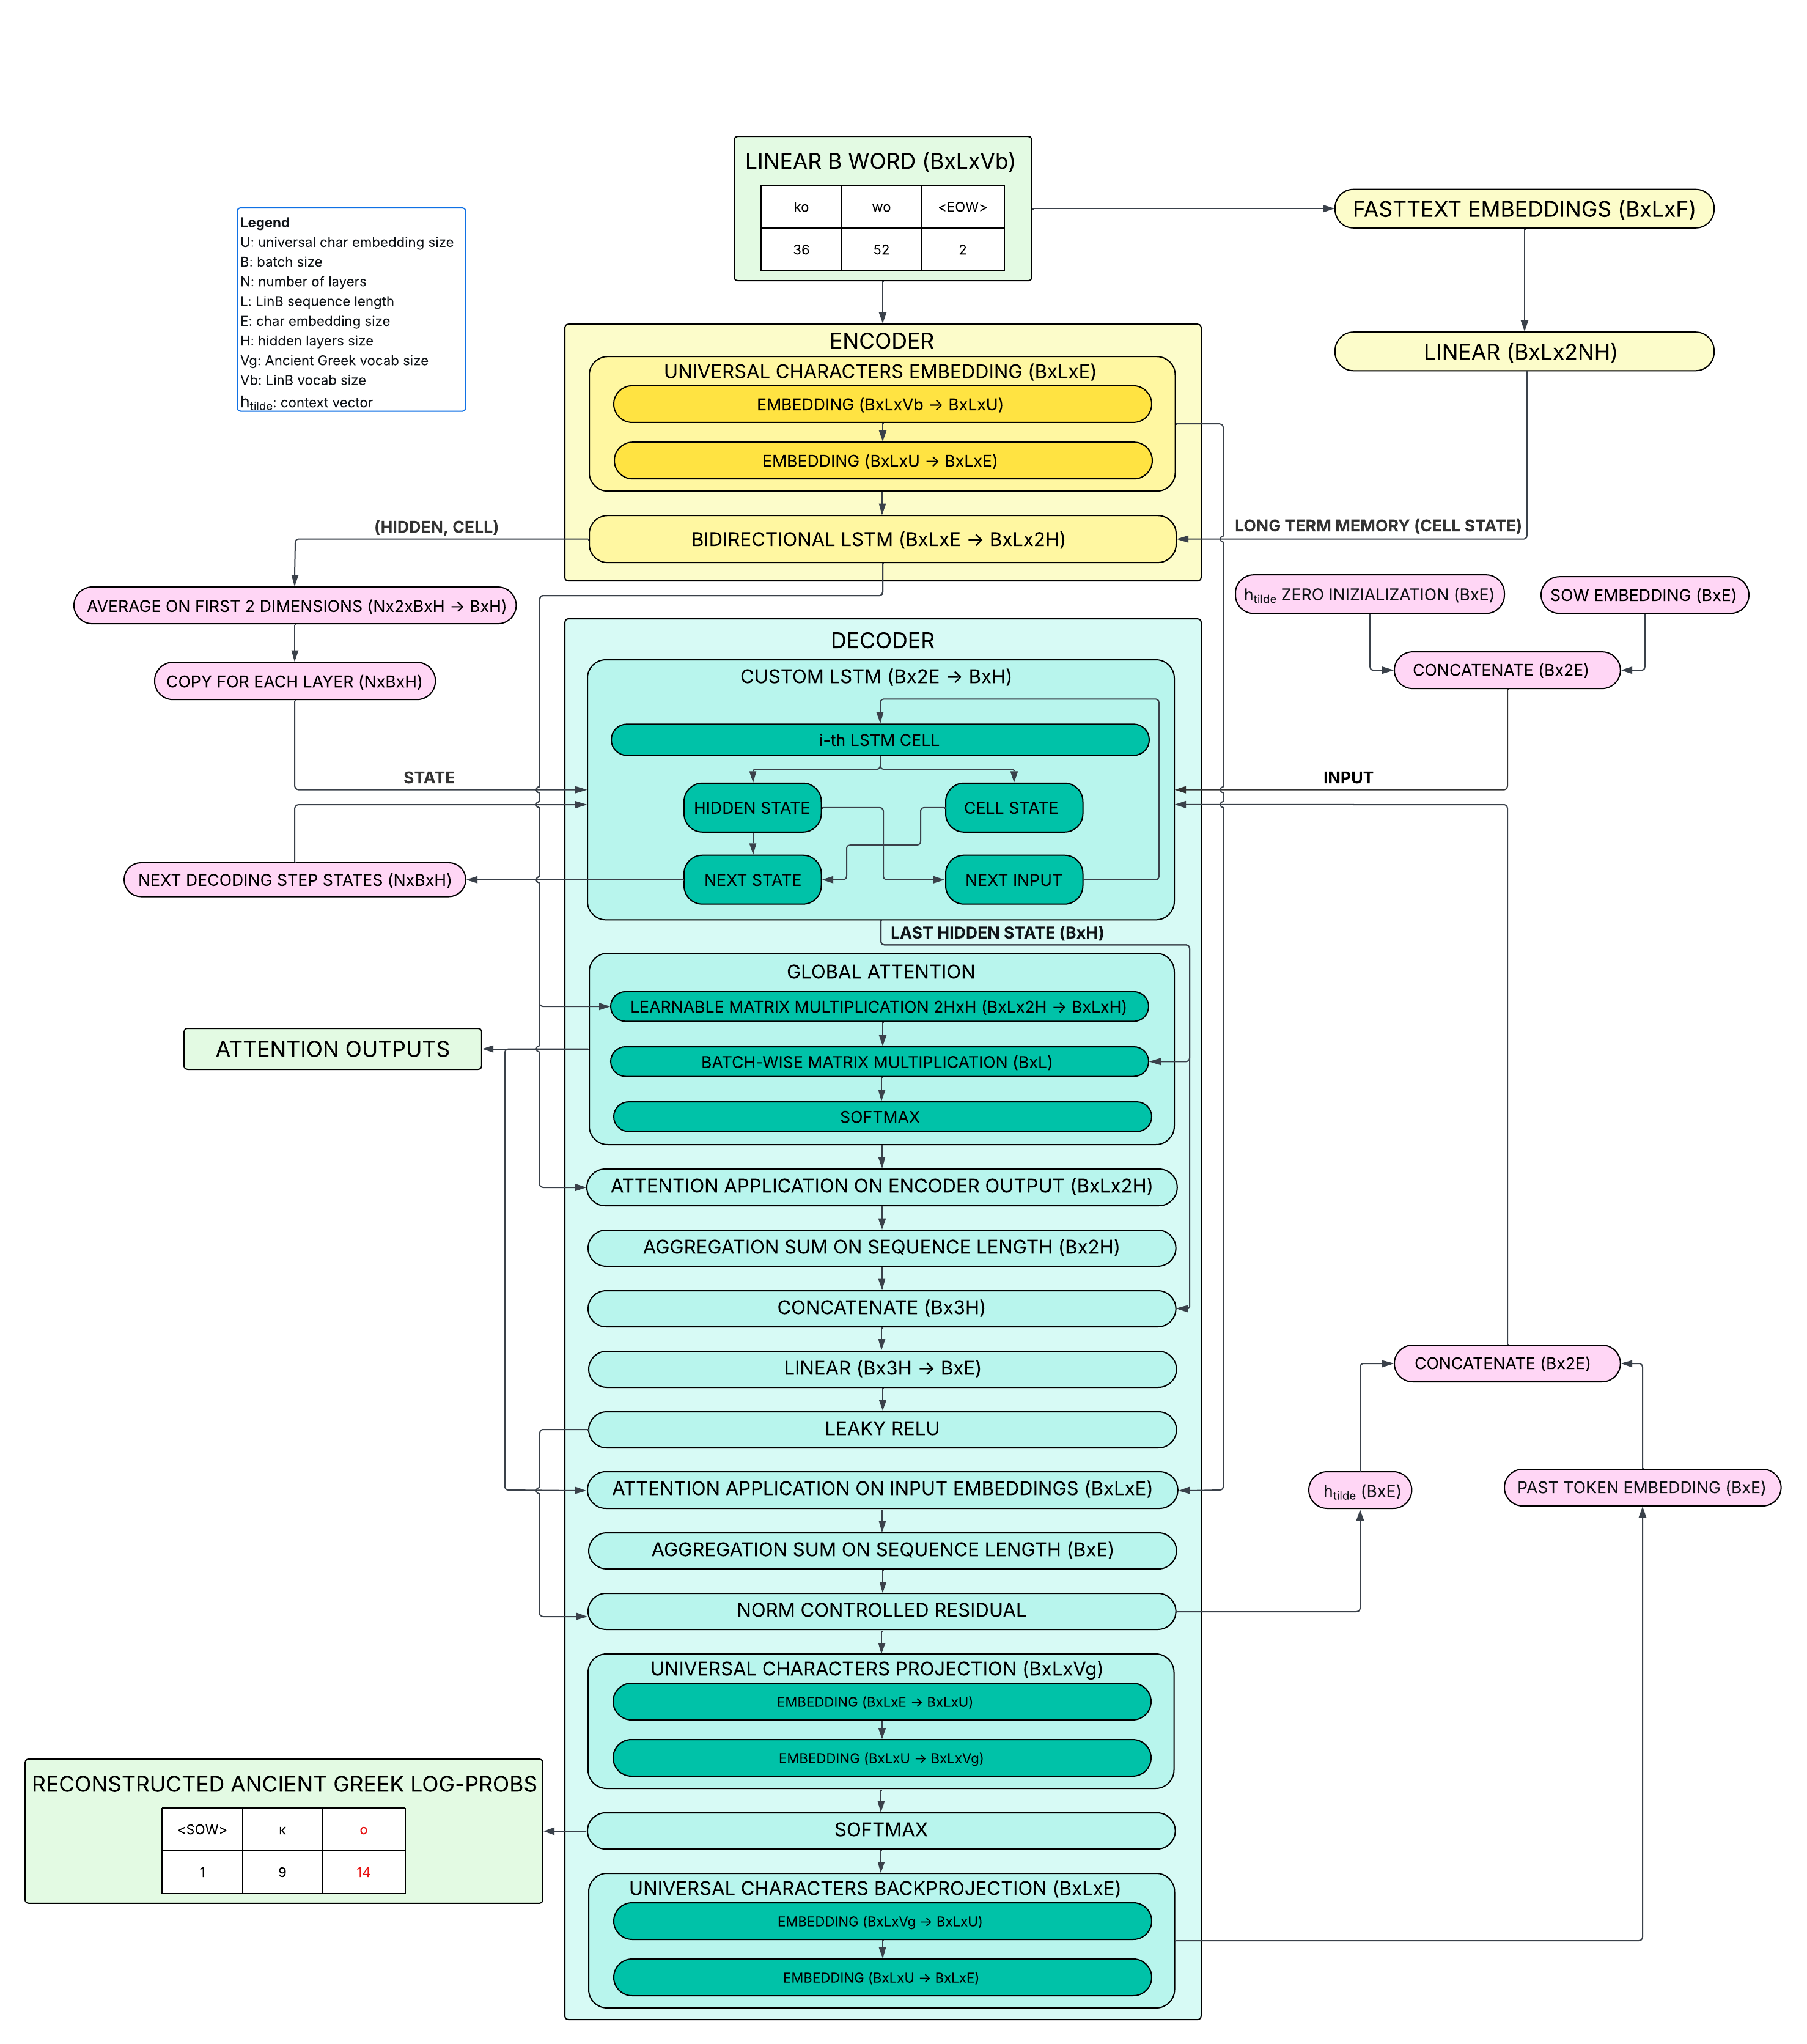
\includegraphics[width=1.2\textwidth]{Images/luo_model.png} % Adjust width and filename
    \caption{Graphical representation of the model architecture.}
    \label{fig:luo_model}
\end{figure}

\begin{figure}[H]
    \centering
    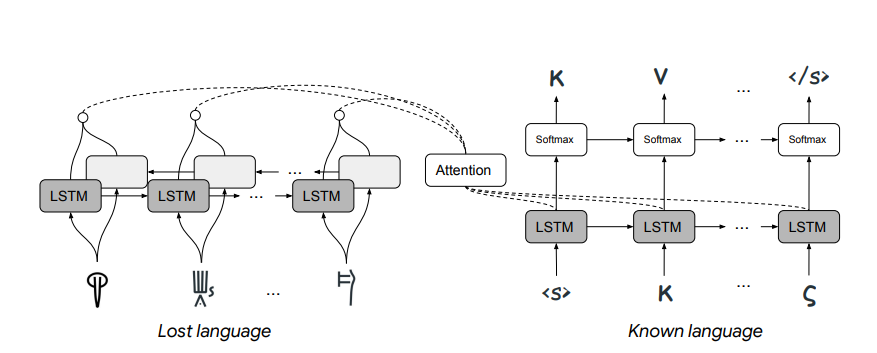
\includegraphics[width=0.8\textwidth]{Images/luo_model_overview.png} % Adjust width and filename
    \caption{Overview of the model architecture.\protect\footnotemark}
    \label{fig:luo_model_overview}
\end{figure}
\footnotetext{Figure \ref{fig:luo_model_overview} prepared by Jiaming Luo.}

\subsection{Output Refinement}
The model supports three output modes.
The first is a corpus-constrained maximum-likelihood selection (MLE) based on the decoder's character distributions.
Given the decoder outputs $\{p_t\}$ for $t=1,\ldots,T_{\max}$, where $p_t\in\mathbb{R}^{V_g}$ is a probability vector over the Greek vocabulary at step $t$, each candidate word $y_j=(y_{j, 1},\ldots,y_{j, T_w})$ in the lexicon is scored by the product of the probabilities of its characters:
\[
\mathbf{P}_{\theta}(y_j \mid x_i)
= \prod_{t=1}^{T_w} p_t[y_{j, t}] \, ,
\]
Equivalently, if $E(y_j)\in\{0,1\}^{T_w\times V_g}$ is the one-hot matrix of $y_j$ (row $t$ is one-hot for $y_{j,t}$), indicating with $E_t(y_j)$ the $t$-th row, then
\[
\log \mathbf{P}_{\theta}(y_j \mid x_i)
= \sum_{t=1}^{T_w} E_t(y_j)\,\log p_t \, ,
\]
which is the form used in practice for numerical stability.

As explained in Section \ref{sec:generative-framework}, the other two output modes are defined via a minimum-cost flow over a bipartite graph.
Edges from source to lost-language nodes have unit capacity; edges from known-language nodes to sink have capacity $C$ (a hyperparameter); the edges between languages have capacity $1$.
The two modes differ only in how the edge costs $d_{ij}$ (from $x_i$ to $y_j$) are computed.

In the first flow mode, set $d_{ij}=-\log \mathbf{P}_{\theta}(y_j\mid x_i)$, i.e., reuse the corpus-constrained MLE score.

In the second flow mode, the character probabilities $\{p_t\}$ are used to sample multiple candidate Ancient Greek words, which are then compared to each lexicon word $y_j$ via normalized edit distance.
For each lost language item $x_i$ we estimate, for every lexicon word $y_j$, an expected normalized edit distance under the decoder's output distributions:

\begin{enumerate}[leftmargin=2em]
\item \textbf{Sample $S$ strings from the decoder.}
Using the per-step character distributions $\{p_t\}_{t=1}^{T_{\max}}$, optionally sharpened by a temperature $\alpha>1$, independently draw $S$ strings and truncate at \textsc{eos}:
$s_{i,k}=(s_{i,k,1},\ldots,s_{i,k,T_{s_{i,k}}})$, $k=1,\ldots,S$.

\item \textbf{Score each sample by its (log-)likelihood.}
With an \textsc{eos} mask $m_{i,k,t}\in\{0,1\}$, define
\[
\log \mathbf{P}(s_{i,k}\!\mid x_i)
\;=\;
\sum_{t=1}^{T_{\max}} m_{i,k,t}\,\log p_t\!\bigl[s_{i,k,t}\bigr].
\]

\item \textbf{Compute normalized edit distances to each candidate.}
For every lexicon word $y_j$ and each sample $s_{i,k}$,
\[
\delta\bigl(y_j,s_{i,k}\bigr)
\;=\;
\frac{\mathrm{Lev}\bigl(y_j,s_{i,k}\bigr)}
     {\min\!\bigl(\lvert y_j\rvert,\lvert s_{i,k}\rvert\bigr)+1}\,.
\]
Also the "original" candidate with zero distance is included:
$\delta\bigl(y_j,s_{i,0}\bigr)\equiv 0$ and score
$\log \mathbf{P}(s_{i,0}\!\mid x_i)\equiv \log \mathbf{P}_{\theta}(y_j\!\mid x_i)$.

\item \textbf{Weight and average.}
Convert the $(1+S)$ log-scores
$\{\log \mathbf{P}(s_{i,k}\!\mid x_i)\}_{k=0}^{S}$
to non-negative weights $\{w_{i,k}\}_{k=0}^{S}$ proportional to their likelihoods and normalized to sum to $1$.
Set the edge cost to the expected normalized edit distance:
\[
d_{ij}
\;=\;
\sum_{k=0}^{S} w_{i,k}\,\delta\bigl(y_j,s_{i,k}\bigr).
\]
\end{enumerate}


\begin{figure}[H]
    \centering
    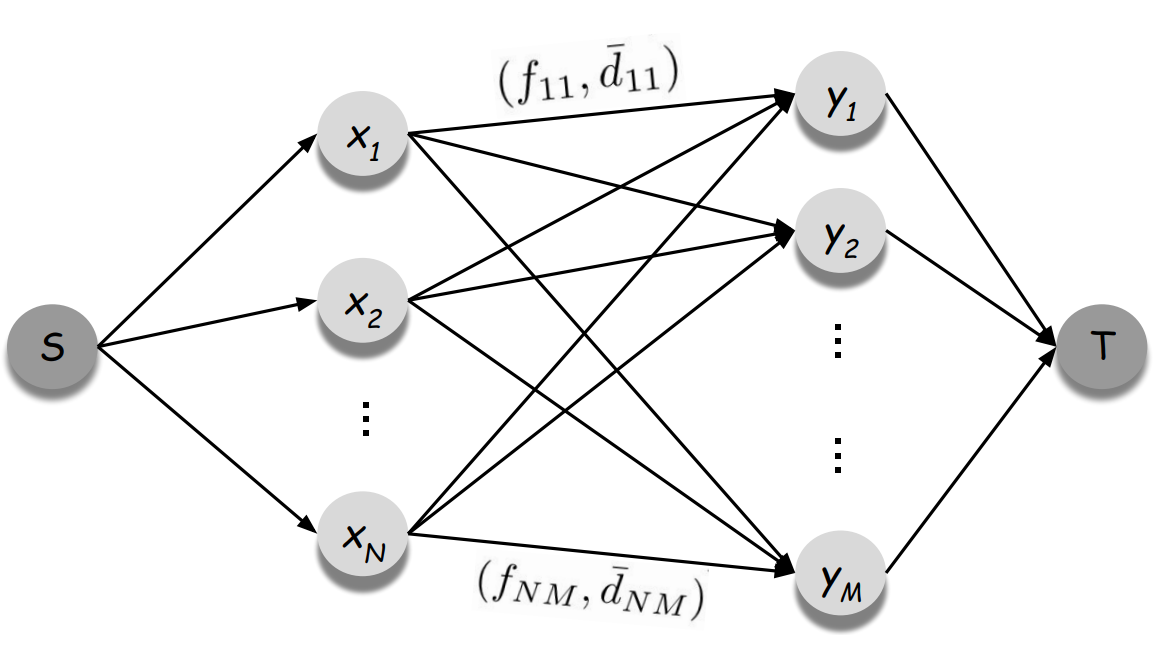
\includegraphics[width=1\textwidth]{Images/luo_flow.png} % Adjust width and filename
    \caption{Overview of the min-cost flow architecture.\protect\footnotemark}
    \label{fig:luo_flow}
\end{figure}
\footnotetext{Figure \ref{fig:luo_flow} prepared by Jiaming Luo.}

\subsection{The loss functions}
The model is trained by minimizing the objective function introduced in Section \ref{sec:generative-framework}.
However, the flow solver returns sparse values, as the flow values for the edges are mostly zeros.
This would likely discard most valid cognate pairs during training.

To address this issue, Luo proposed to use an exponential decay for the flow values in the loss function computation.
These values are updated in each E-step and used in the M-step to compute the loss.
Concretely, the flow values at iteration $\tau$ are updated as follows:
\[
f_{ij}^{(\tau)} \;=\; \gamma\,f_{ij}^{(\tau-1)} + (1-\gamma)\,\tilde{f}_{ij}^{(\tau)} \quad \forall\, i,j,
\]
where $\tilde{f}_{ij}^{(\tau)}$ are the flow values returned by the flow solver at iteration $\tau$, and $\gamma\in[0,1)$ is a hyperparameter that controls the decay rate.

The loss function is then defined as:
\begin{gather*}
\mathcal{L}_{\mathrm{NLL}} =
- \sum_{y_j \in \mathcal{Y}} f_j^{(\tau)} \log \left(\sum_{x_i \in \mathcal{X}} \exp \!\left(\log f_{ij}^{(\tau)} + \log \mathbf{P}_{\theta}(y_j \mid x_i) \right) \right) \;= \\[2pt]
- \sum_{y_j \in \mathcal{Y}} f_j^{(\tau)} \log \left(\sum_{x_i \in \mathcal{X}} f_{ij}^{(\tau)} \cdot \mathbf{P}_{\theta}(y_j \mid x_i) \right) = - \log \left(\prod_{y_j \in \mathcal{Y}} \left( \sum_{x_i \in \mathcal{X}} f_{ij}^{(\tau)} \cdot \mathbf{P}_{\theta}(y_j \mid x_i) \right)^{f_j^{(\tau)}} \right) \, ,
\end{gather*}
where $f_j^{(\tau)} = \sum_{x_i \in \mathcal{X}} f_{ij}^{(\tau)}$ is the aggregated flow into node $y_j$ and acts as a weight for the loss of that word.

An additional loss component is introduced to encourage monotonic alignments.
This component, called monotonic alignment regularization, penalizes unaligned positions of predicted characters.
The loss acts directly on the attention weights $\alpha_t$ produced by the Global Attention module.

Concretely, the attention weights are interpreted, for each word of the lost language $x_i$, as the alignment probability over the input sequence at each decoding step $t$.
Therefore, $\alpha_t^{(i)}(k) = \mathbf{P}(a_t^{(i)}=k \mid x_i)$, where $a_t^{(i)}$ is the alignment position at step $t$ for word $x_i$.
This probability is used to derive the expected alignment position for each character of the output sequence:
\[
pos_t^{(i)} \;=\; \sum_{k=1}^{L} k \cdot \alpha_t^{(i)}(k)
\;=\; \sum_{k=1}^{L} k \cdot \mathbf{P}(a_t^{(i)}=k \mid x_i) \, .
\]
The monotonic alignment regularization loss is then defined as:
\[
\mathcal{L}_{\mathrm{MAR}} \;=\; \sum_{x_i \in \mathcal{X}} \sum_{t=1}^{T_{\max}} \bigl(pos_t^{(i)} - pos_{t-2}^{(i)} - 1\bigr)^2 \, ,
\]
to accommodate the fact that Linear B is a syllabic language and usually one Linear B sign corresponds to two Greek letters.
An example of alignment between a Linear B word and its Ancient Greek cognate is presented in Figure \ref{fig:alignment_example}.
\begin{figure}[H]
    \centering
    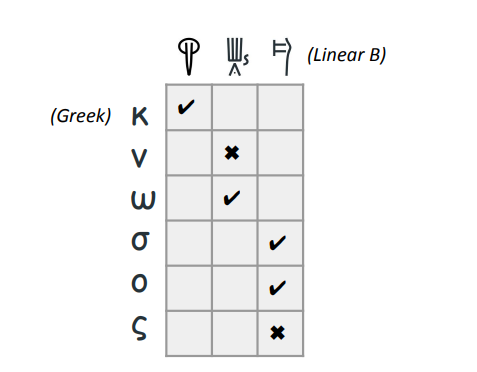
\includegraphics[width=0.6\textwidth]{Images/alignment.png} % Adjust width and filename
    \caption{Example of alignment between a Linear B word and its Ancient Greek cognate. \cmark\ and \xxmark\ indicate correct and incorrect alignment positions, respectively. The misalignment between \textlinb{\Bno} (no) and \textgreek{ν} corresponds to a deletion error, while the misalignment between \textlinb{\Bso} (so) and \textgreek{ς} corresponds to an insertion error.\protect\footnotemark}
    \label{fig:alignment_example}
\end{figure}
\footnotetext{Figure \ref{fig:alignment_example} prepared by Jiaming Luo.}

The final loss function is a weighted sum of the two components:
\[
\mathcal{L} \;=\; \mathcal{L}_{\mathrm{NLL}} + \lambda\,\mathcal{L}_{\mathrm{MAR}} \, ,
\]
where $\lambda$ is a hyperparameter that controls the trade-off between the two loss components.

\subsection{Training Procedure}
As anticipated in Section \ref{sec:generative-framework}, training proceeds in an EM-style loop.
We initialize the alignment flow matrix with a simple prior and then alternate between:

\begin{itemize}[leftmargin=2em]
  \item \textbf{M-step:} fit the seq2seq parameters \(\theta^{(\tau)}\) by maximizing the corpus likelihood under the fixed flows \(f^{(\tau-1)}\).
  \item \textbf{E-step:} recompute edge costs from \(\theta^{(\tau)}\), solve a minimum-cost flow to obtain raw flows \(\tilde f^{(\tau)}\), and update the stable flows via exponential smoothing:
  \[
    f_{ij}^{(\tau)} \;=\; \gamma\,f_{ij}^{(\tau-1)} \;+\; (1-\gamma)\,\tilde f_{ij}^{(\tau)} \, .
  \]
\end{itemize}

To reduce overfitting to the previous iterate and to avoid poor local minima, the neural parameters are re-initialized at the start of each new M-step.
This procedure is summarized in the pseudocode of Algorithm \ref{alg:em-flow}.

This behavior yields distinctive loss/accuracy trajectories for each split (Figure \ref{fig:validation-acc}): curves change sharply at E-M boundaries because flows are recomputed and model parameters are re-initialized.
A practical mitigation is to aggregate within each E-step (e.g., average across its M-steps) or, more conservatively, to report only the final M-step metrics.

The full training procedure and loss computations are graphically illustrated in Figure \ref{fig:luo_framework}.

\begin{figure}[H]
    \centering
    \begin{subfigure}[b]{0.46\textwidth}
        \centering
        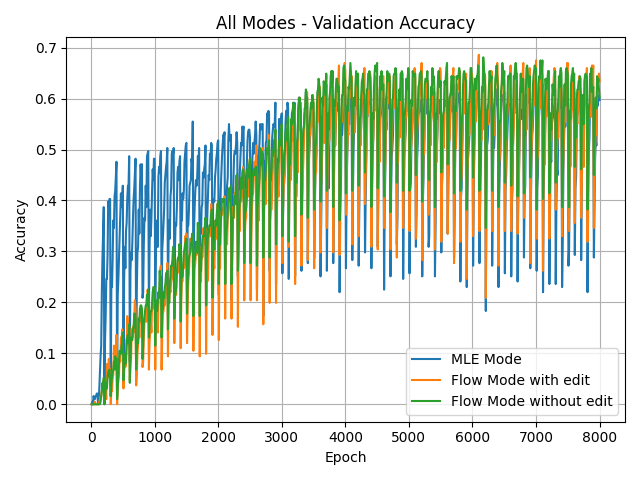
\includegraphics[width=\textwidth]{Images/accuracy_all_modes_validation.png}
        \caption{Accuracy at each M-step.}
        \label{fig:validation-acc-m}
    \end{subfigure}\hfill
    \begin{subfigure}[b]{0.46\textwidth}
        \centering
        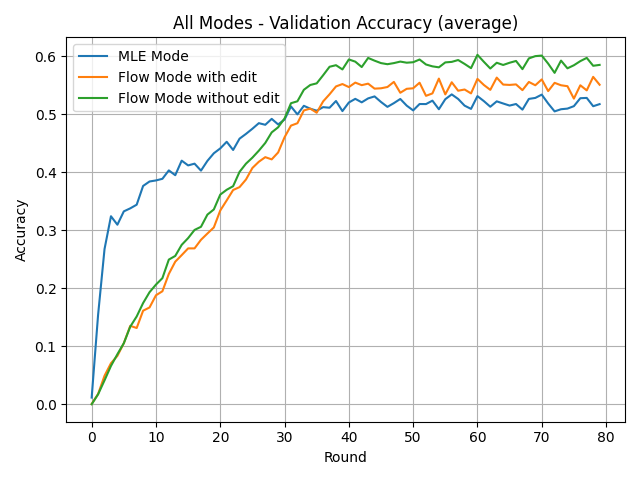
\includegraphics[width=\textwidth]{Images/average_accuracy_all_modes_validation.png}
        \caption{Average accuracy at each E-step.}
        \label{fig:validation-acc-e}
    \end{subfigure}
    \caption{Validation accuracy during training. (a) Raw per M-step accuracy. \\ 
    (b) Accuracy averaged within each E-step.}
    \label{fig:validation-acc}
\end{figure}

\begin{algorithm}[H]
    \SetAlgoNoLine
    \DontPrintSemicolon
    \SetAlgoNoEnd
    
    \SetKwInOut{Input}{Input}
    \SetKwInOut{Output}{Output}
    \SetKwProg{Fn}{Function}{}{}

    \Input{$\mathcal{X}, \mathcal{Y}$ (vocabularies);\ $T$ (number of iterations);\ $N$ (number of cognate pairs to identify)}
    \Output{$f^{(T)}_{ij}$ (final soft alignments/flows)}
    
    \BlankLine
    $f^{(0)}_{ij} \gets \dfrac{N}{|\mathcal{X}|\,|\mathcal{Y}|}$ \tcp*{Initialize uniform flow}
    \For{$\tau \gets 1$ \KwTo $T$}{
        $\theta^{(\tau)} \gets \mathrm{MLE\mbox{-}TRAIN}\!\bigl(f^{(\tau-1)}_{ij}\bigr)$\;
        $d^{(\tau)}_{ij} \gets \mathrm{EDIT\mbox{-}DIST}\!\bigl(x_i, y_j;\, \theta^{(\tau)}\bigr)$\;
        $\tilde f^{(\tau)}_{ij} \gets \mathrm{MIN\mbox{-}COST\mbox{-}FLOW}\!\bigl(d^{(\tau)}_{ij}\bigr)$\;
        $f^{(\tau)}_{ij} \gets \gamma\, f^{(\tau-1)}_{ij} + (1-\gamma)\,\tilde f^{(\tau)}_{ij}$\;
        \textsc{Reset}$\!\bigl(\theta^{(\tau)}\bigr)$\;
    }
    \Return{$f^{(T)}_{ij}$}\;

    \BlankLine
    \Fn{MLE-TRAIN{$\bigl(f^{(\tau)}_{ij}\bigr)$}}{
        $\displaystyle \theta^{(\tau)} \gets \arg\max_{\theta}\ \prod_{y_j\in\mathcal{Y}} \mathbf{P}_{\theta}\!\bigl(y_j \mid \mathcal{X}, \mathcal{F}\bigr)$\;
        \Return{$\theta^{(\tau)}$}\;
    }

    \caption{Iterative training with EM and minimum-cost flow \protect\footnotemark}\label{alg:em-flow}
\end{algorithm}
\footnotetext{Algorithm \ref{alg:em-flow} taken by Jiaming Luo.}

\begin{figure}[H]
    \begin{adjustbox}{center}
        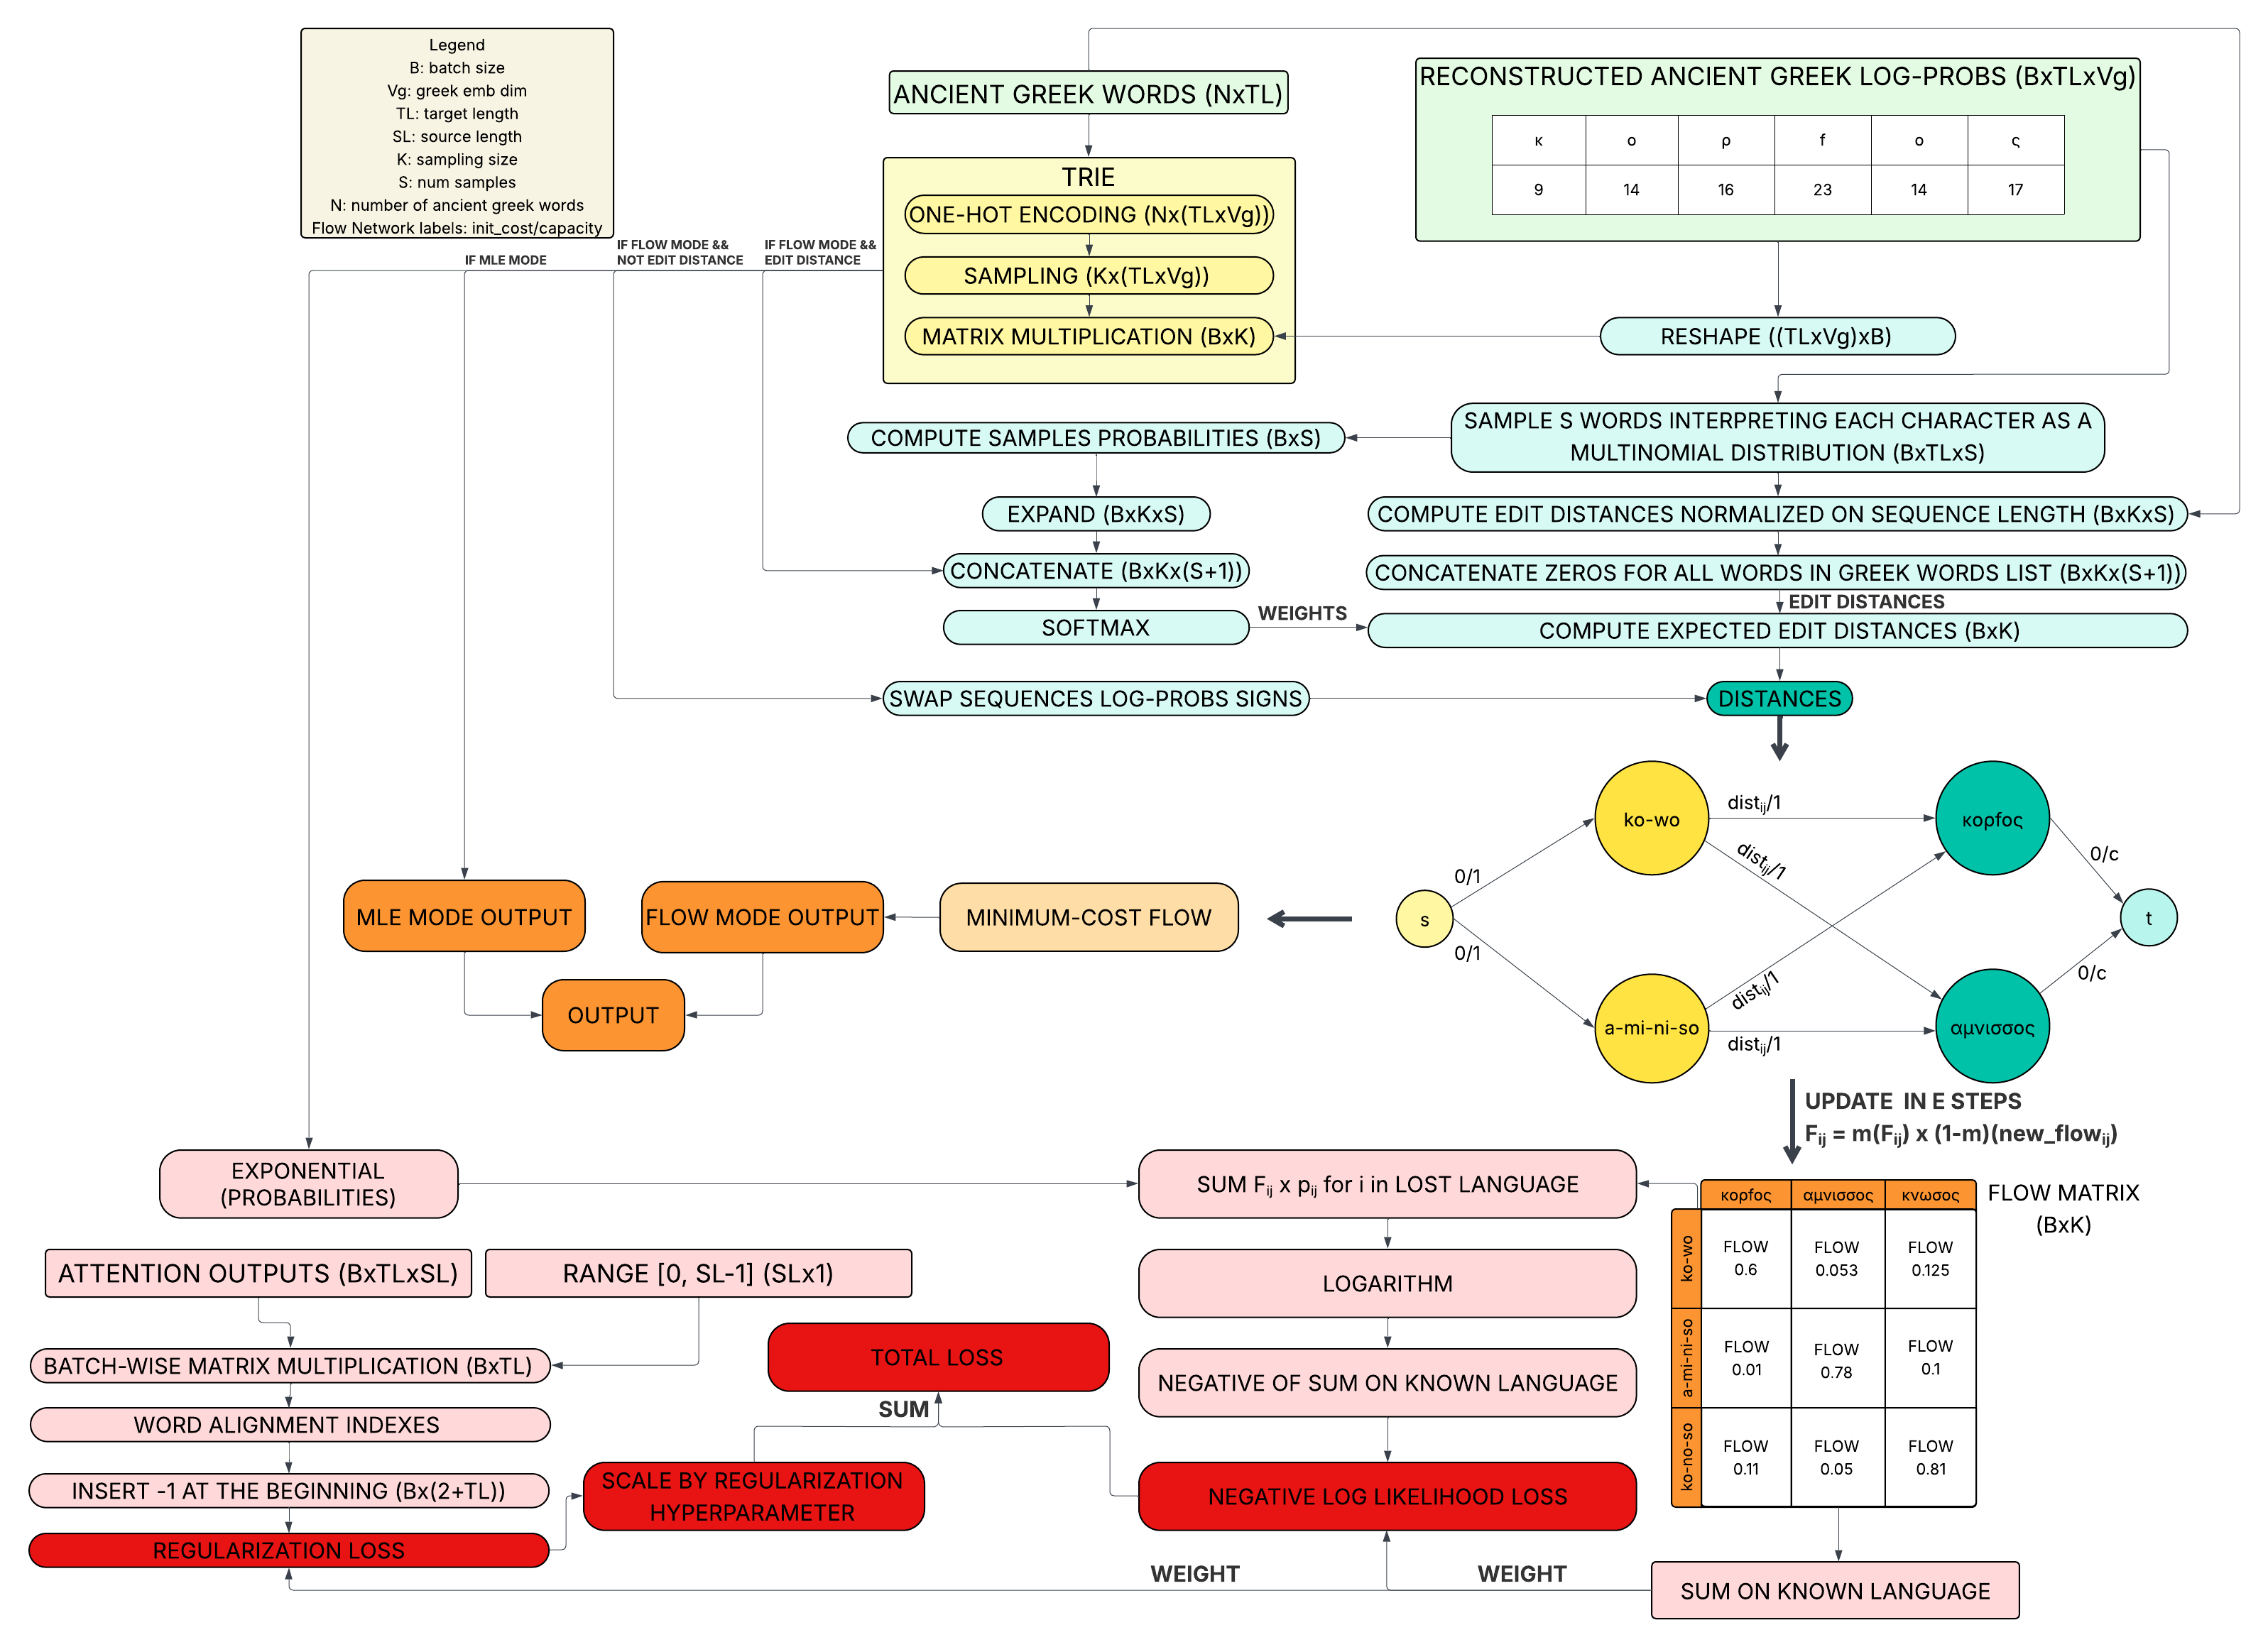
\includegraphics[width=1.25\textwidth]{Images/luo_framework.png}
    \end{adjustbox}
    \caption{Graphical outline of Luo's training procedure.}
    \label{fig:luo_framework}
\end{figure}

\subsection{Results} \label{sec:results}
In this section, I present the results of my experiments with the cognate matching model on three datasets:
\begin{itemize}[leftmargin=2em]
    \item \textbf{Luo's dataset} \cite{luo}, which contains 919 cognate pairs.
    \item \textbf{Luo's corrected dataset}, which contains 976 cognate pairs, obtained by applying some manual corrections on Luo's dataset.
    \item \textbf{Our dataset}, which contains 1911 cognate pairs from both Luo's dataset and Tselentis' \cite{tselentis} dataset, with additional manually identified pairs using the brute-force algorithm, and Ventris and Chadwick's notes \cite{chadwick-notes}.
\end{itemize}

Overall, I ran two sets of experiments.
In the first set, I compared the performance of the model on the full datasets, without defining train/validation/test splits.
In the second set, I defined train/validation/test splits for both Luo's dataset and our dataset, and compared the performance of the model on each split.
The sizes of the splits are the following: 80\% of samples for training, 10\% for validation, and 10\% for test.
For both sets of experiments, I compared the model across all output modes, with and without initializing the LSTM cell states with FastText embeddings.
The results are presented in the tables below.

\begin{table}[h!]
\centering
\begin{tabular}{|c|c|c|c|}
\hline
\textbf{LSTM Initialization} & \textbf{MLE} & \textbf{Flow without edit} & \textbf{Flow with edit} \\
\hline
zero   & 0.830 & 0.831 & 0.781 \\
custom & 0.822 & 0.822 & 0.820 \\
\hline
\end{tabular}
\caption{Comparison of model performance on Luo's original dataset.}
\end{table}

\begin{table}[h!]
\centering
\begin{tabular}{|c|c|c|c|}
\hline
\textbf{LSTM Initialization} & \textbf{MLE} & \textbf{Flow without edit} & \textbf{Flow with edit} \\
\hline
zero   & 0.827 & 0.828 & 0.781 \\
custom & 0.841 & 0.841 & 0.840 \\
\hline
\end{tabular}
\caption{Comparison of model performance on Luo's corrected dataset.}
\end{table}

\begin{table}[h!]
\centering
\begin{tabular}{|c|c|c|c|}
\hline
\textbf{LSTM Initialization} & \textbf{MLE} & \textbf{Flow without edit} & \textbf{Flow with edit} \\
\hline
zero   & 0.694 & 0.711 & 0.671 \\
custom & 0.662 & 0.662 & 0.672 \\
\hline
\end{tabular}
\caption{Comparison of model performance on our dataset.}
\end{table}

It can be observed that, despite the stabilization effect of the custom LSTM initialization, when the model converges with a zero initialization it achieves better performance.
Particularly, the model attains higher accuracy on our more challenging and extensive dataset, reaching 71.1\% with the flow without edit mode.
The final accuracy and loss at each E-step during training on our dataset with zero initialization of the cell states are presented in Figure \ref{fig:acc-loss-all}.

\begin{figure}[H]
    \centering
    \begin{subfigure}[b]{0.46\textwidth}
        \centering
        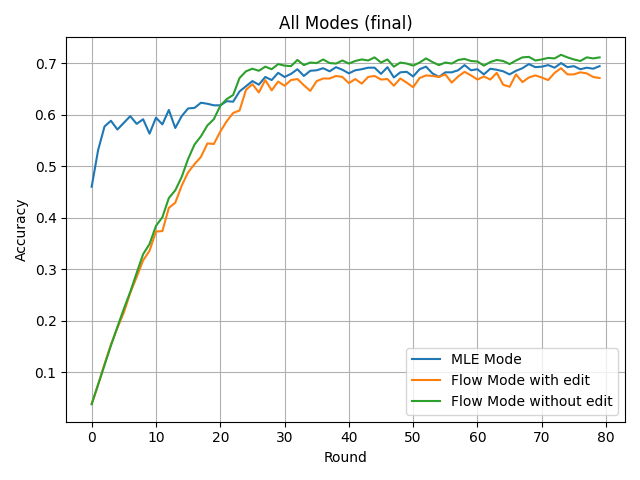
\includegraphics[width=\textwidth]{Images/final_accuracy_all_modes.png}
        \caption{Final accuracy at each E-step.}
        \label{fig:final-acc-all}
    \end{subfigure}\hfill
    \begin{subfigure}[b]{0.46\textwidth}
        \centering
        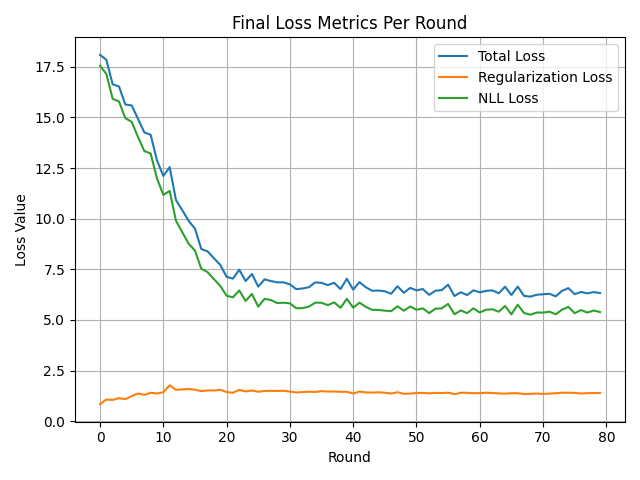
\includegraphics[width=\textwidth]{Images/final_loss_all_metrics.png}
        \caption{Final loss at each E-step.}
        \label{fig:final-loss-all}
    \end{subfigure}
    \caption{Metrics for the zero-initialized model during training on our dataset. \\
    (a) Accuracy. (b) Loss.}
    \label{fig:acc-loss-all}
\end{figure}

The same trends are observed in the experiments with train/validation/test splits.
However, due to the reduced size of the training set and the removal of some cognate pairs from it, the overall performance is lower.
While the zero-initialized model remains strong, the custom-initialized variant degrades substantially.
The results are presented in the tables below.

\begin{table}[h!]
\centering
\begin{tabular}{|c|c|c|c|c|}
\hline
\textbf{LSTM Init} & \textbf{Split} & \textbf{MLE} & \textbf{Flow w/o edit} & \textbf{Flow w/ edit} \\
\hline
\multirow{3}{*}{zero}
& Train      & 0.789 & 0.790 & 0.735 \\
& Validation & 0.663 & 0.674 & 0.696 \\
& Test       & 0.761 & 0.761 & 0.728 \\
\hline
\multirow{3}{*}{custom}
& Train      & 0.411 & 0.423 & 0.435 \\
& Validation & 0.391 & 0.424 & 0.435 \\
& Test       & 0.359 & 0.359 & 0.435 \\
\hline
\end{tabular}
\caption{Performance (Train/Validation/Test) on Luo's original dataset.}
\end{table}

\begin{table}[h!]
\centering
\begin{tabular}{|c|c|c|c|c|}
\hline
\textbf{LSTM Init} & \textbf{Split} & \textbf{MLE} & \textbf{Flow w/o edit} & \textbf{Flow w/ edit} \\
\hline
\multirow{3}{*}{zero}
& Train      & 0.782 & 0.785 & 0.732 \\
& Validation & 0.717 & 0.717 & 0.663 \\
& Test       & 0.739 & 0.739 & 0.696 \\
\hline
\multirow{3}{*}{custom}
& Train      & 0.457 & 0.469 & 0.486 \\
& Validation & 0.446 & 0.467 & 0.511 \\
& Test       & 0.370 & 0.380 & 0.511 \\
\hline
\end{tabular}
\caption{Performance (Train/Validation/Test) on Luo's corrected dataset.}
\end{table}

\begin{table}[h!]
\centering
\begin{tabular}{|c|c|c|c|c|}
\hline
\textbf{LSTM Init} & \textbf{Split} & \textbf{MLE} & \textbf{Flow w/o edit} & \textbf{Flow w/ edit} \\
\hline
\multirow{3}{*}{zero}
& Train      & 0.645 & 0.658 & 0.639 \\
& Validation & 0.597 & 0.602 & 0.634 \\
& Test       & 0.625 & 0.646 & 0.646 \\
\hline
\multirow{3}{*}{custom}
& Train      & 0.238 & 0.275 & 0.367 \\
& Validation & 0.262 & 0.262 & 0.377 \\
& Test       & 0.224 & 0.234 & 0.370 \\
\hline
\end{tabular}
\caption{Performance (Train/Validation/Test) on our dataset.}
\end{table}

This significant drop in the custom-initialized runs is consistent with a loss–accuracy divergence caused by a representation mismatch.
FastText injects word-level semantic priors into a character-mapping task.
As a result, the model becomes confidently wrong on many instances: the negative log-likelihood can keep improving (higher confidence), while accuracy on held-out data declines (worse argmax decisions).
In short, the initialization biases the decoder toward signals that are orthogonal to the target grapheme-level correspondences, leading to miscalibration and poorer generalization, due to representational mismatch.

The final accuracy of all splits, using MLE mode, and the final accuracy of the test split, using all output modes, of the zero-initialized model during training on our dataset are presented in Figure \ref{fig:acc-loss-splits}.
\begin{figure}[H]
    \centering
    \begin{subfigure}[b]{0.46\textwidth}
        \centering
        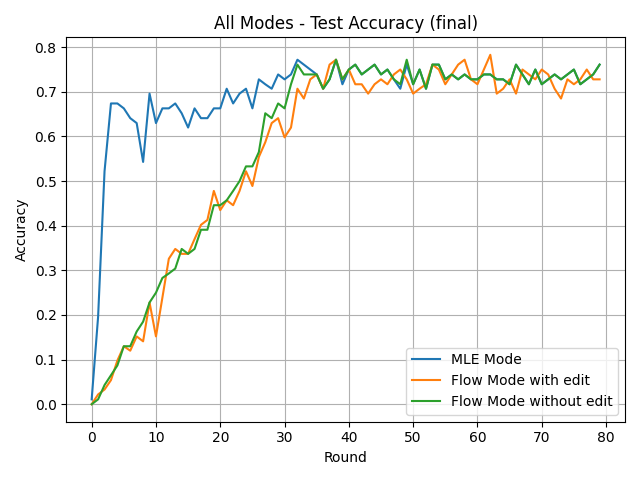
\includegraphics[width=\textwidth]{Images/final_accuracy_all_modes_test.png}
        \caption{Final accuracy at each E-step for the test set in all modes.}
        \label{fig:final-acc-test-all}
    \end{subfigure}\hfill
    \begin{subfigure}[b]{0.46\textwidth}
        \centering
        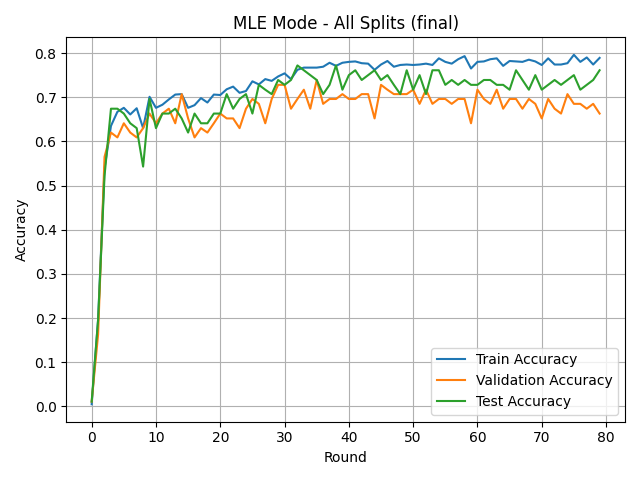
\includegraphics[width=\textwidth]{Images/final_accuracy_mle_mode_all_splits.png}
        \caption{Final accuracy at each E-step in MLE mode for all splits.}
        \label{fig:final-acc-mle-all}
    \end{subfigure}
    \caption{Metrics for the zero-initialized model during training on our dataset. \\ 
    (a) Accuracy for the test set in all modes. (b) Accuracy in MLE mode for all splits.}
    \label{fig:acc-loss-splits}
\end{figure}
\chapter{Auxialiary Classifiers}
PALLE
\chapter{Translation Pipeline} \label{chap:pipeline}
In this chapter, I evaluate the ability of large language models (LLMs) to translate Linear B into Ancient Greek. 
The full pipeline proceeds as follows:

\begin{itemize}[leftmargin=2em]
  \item \textbf{Vocabulary extraction.} Gather every distinct word form attested in the Linear B documents (after cleaning/normalization).
  \item \textbf{Brute-force cognates.} For forms not already covered by our dataset, run the brute-force search against the Ancient Greek lexicon to obtain initial candidates (detailed in Section \ref{sec:bruteforce-cognates}).
  \item \textbf{Candidate aggregation.} For each word, collect possible cognates from: (i) the dataset's suggested cognates, (ii) the raw output of the cognate-matching model trained on our dataset, together with the output of all decoding modes, and (iii) a version of the cognate matcher retrained on the enlarged set. Duplicates are removed from the candidate set.
  \item \textbf{Auxiliary signals.} Train the Linear-SVM auxiliary classifiers on their labeled sets, then predict part of speech, noun type, and inflection for every word in the corpus.
  \item \textbf{Logograms.} Map logograms to their conventional readings/values and include these as fixed translations.
  \item \textbf{LLM prompting.} For each item, assemble a structured prompt containing: the Linear B form, the deduplicated cognate candidates, auxiliary predictions, and relevant morphological guidance. The LLM is asked to (a) select or propose the most plausible Ancient Greek reconstruction, and (b) provide an English translation.
  If the information provided with the prompt is sufficient, the LLM should be able to reconstruct the right inflection for each term and disambiguate the sentence.
\end{itemize}

\begin{figure}[H]
    \begin{adjustbox}{center}
        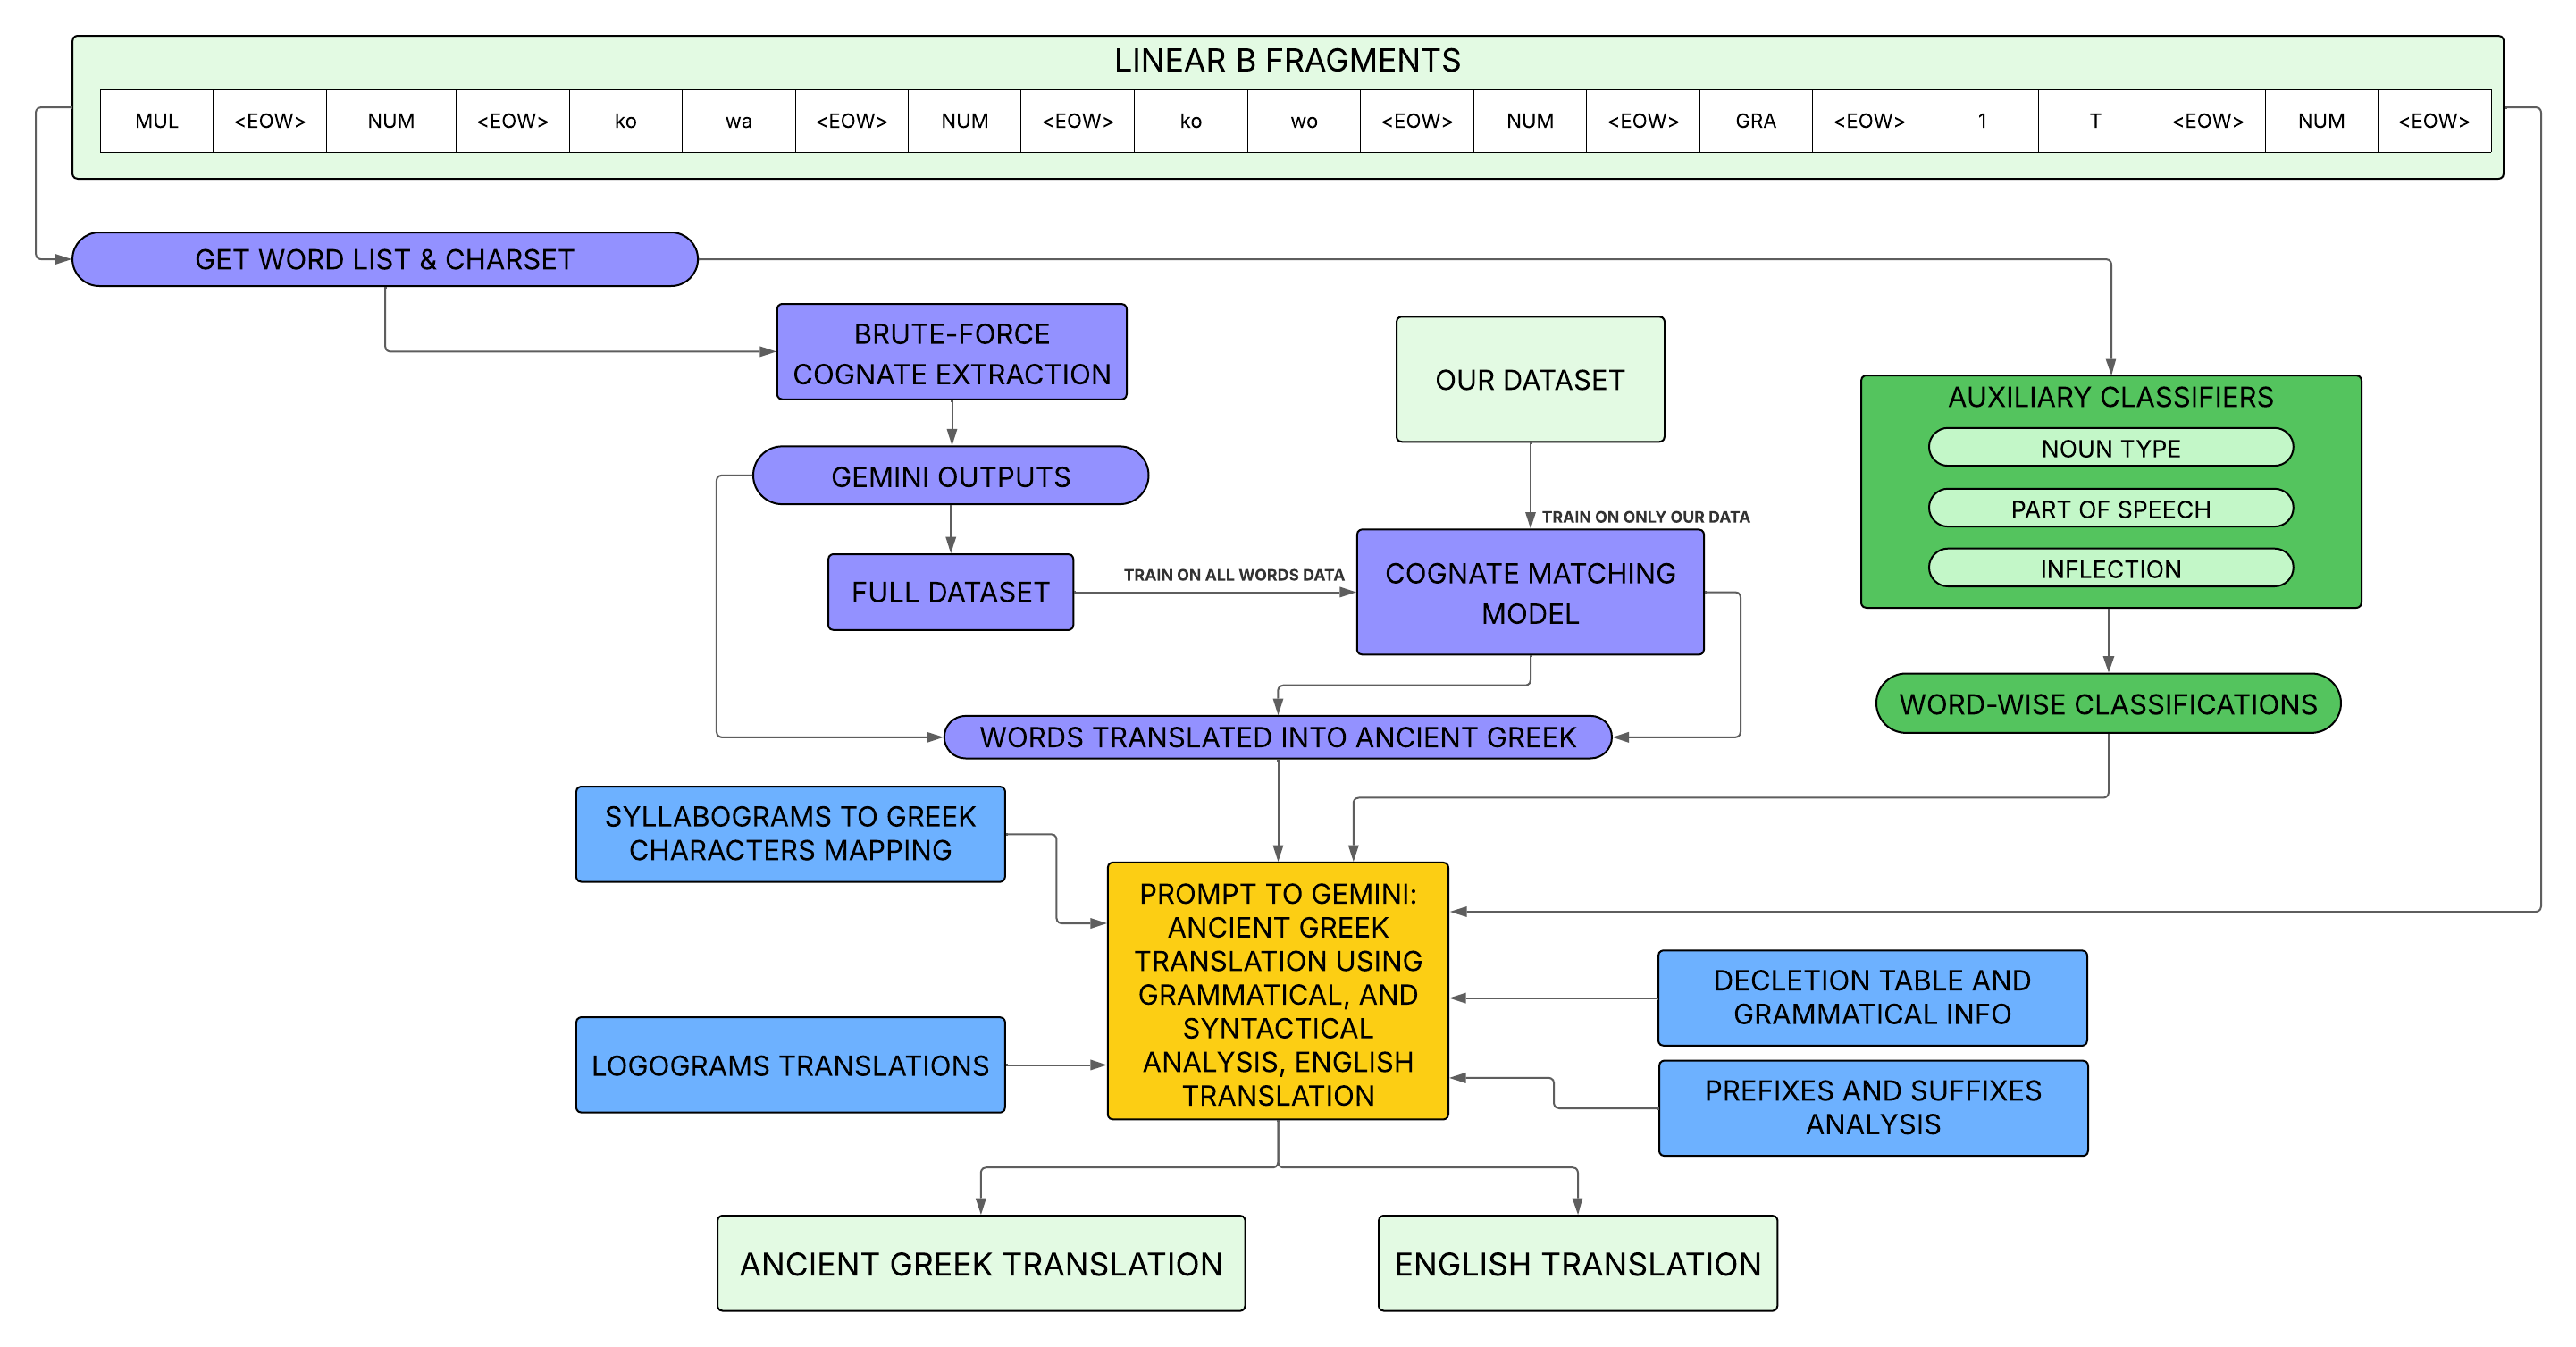
\includegraphics[width=1.2\textwidth]{Images/pipeline.png}
    \end{adjustbox}
    \caption{Overview of the translation pipeline from Linear B to Ancient Greek.}
    \label{fig:pipeline}
\end{figure}

\section{Prompt Design} \label{sec:final-prompt}
This time, instead of a single prompt, the information was given to the large language model using a series of structured messages, each with a specific role.

\paragraph{Historical Context.}
The first message provided to the model was a simple historical context on Linear B and Ancient Greek relationship.
It underlines the fact that Linear B is an early form of Greek, written with a syllabic script, and its administrative nature.
This message was fixed for all words.

\paragraph{Syllabogram Matching.}
The second message contained the Linear B syllabograms and their closest Ancient Greek equivalents, predicted by Luo's model.
It associates to each Linear B syllabogram a list of symbols that could represent it in its Ancient Greek correspondence.
For example, the Linear B syllabogram \textlinb{\Bpa} (pa) is associated with the Ancient Greek letters \textgreek{π}, \textgreek{φ}, and \textgreek{α}, as it usually corresponds to "\textgreek{πα}" or "\textgreek{φα}" syllables.
This was also fixed for all words.

\paragraph{Grammatical Information.}
The third message provided auxiliary grammatical information, such as Linear B declension tables, and additional information about adjectives and verbs, like in the prompt described in Section \ref{sec:aux-dataset}.

\paragraph{Task Definition.}
The fourth message formalized the task. The model receives the Linear~B document as a sequence of tokenized word forms; for each word it is given (i) the aggregated set of candidate Ancient Greek cognates, (ii) auxiliary predictions (part of speech, noun type when applicable, and inflection when applicable), and (iii) a completeness label.
The completeness label is derived from the share $p\!\in\![0,1]$ of occurrences marked as "complete" in the corpus and is bucketed at fixed cutoffs:
\emph{Always Complete} ($p=1$), \emph{Mostly Complete} ($p \geq \frac{2}{3}$), \emph{Uncertain} ($\frac{1}{3} < p < \frac{2}{3}$), \emph{Mostly Incomplete} ($0< p \leq \frac{1}{3}$), \emph{Incomplete} ($p=0$).

The prompt instructs the model on how to complete the translation task, the main steps being:
\begin{itemize}
  \item \textbf{Grammatical analysis.} The first step is to analyze the grammatical features of the Linear B document, separating the words into adjectives, nouns, verbs, and adverbs, and reconstructing the inflection of each noun and adjective, as well as the conjugation of each verb.
  \item \textbf{Syntactic analysis.} The second step is to analyze the document's structure by identifying its sentences and distinguishing the subjects, verbs, and objects mentioned in them.
  \item \textbf{Discourse analysis.} The third step is to analyze the discourse, examining subordinate clauses and establishing coherent logical connections.
  \item \textbf{Linguistic authenticity.} The fourth step is to ensure the selection of an Ancient Greek cognate that preserves morphological patterns and is plausible given the corresponding Mycenaean Greek form.
  \item \textbf{Semantic coherence.} The last step is to ensure that the translation is semantically coherent with the administrative nature of the Linear B documents.
\end{itemize}

These are common steps in translation and linguistic analysis, but they are particularly important in this context due to the similarity between Linear B inflected forms.
The LLM is finally asked given some quality assurance criteria, reflecting the needs of the task, and instructed to use the chain-of-thought technique to reason step by step and refine its translation.

\paragraph{Examples.}
The last information given to the model is a series of examples of translated Linear B fragments.
These examples are selected from a small set of documents provided by Chris Tselentis, together with his Linear B lexicon \cite{tselentis}.

These examples are very short, but they cover a variety of linguistic phenomena and be representative of the administrative purpose of the documents.
The following examples were used:

\begin{enumerate}
  \item \textbf{PY Eb 895+906}: This brief document contains a subordinate clause introduced by a participial form.
  Therefore, it provides key features of Linear B clause structure. \\
  \textbf{Linear B original}: \textlinb{\Ba\Bi\Bqe\Bu} \textlinb{\Be\Bke\Bqe} \textlinb{\Bke\Bke\Bme\Bna} \textlinb{\Bko\Bto\Bna} \textlinb{\Bko\Bto\Bno\Bko} \textlinb{\Bto\Bso\Bde} \textlinb{\Bpe\Bmo} \textlinb{\BPwheat} \textlinb{\BPvolcd} \textlinb{\BNvi}\\
  \textbf{Linear B text}: a-i-qe-u e-ke-qe ke-ke-me-na ko-to-na ko-to-no-o-ko to-so-de pe-mo GRA T 6 \\
  \textbf{Greek translation}: \textgreek{Αἰγεὺς κτοινόοχος ἔχει τε κεκειμένα κτοίνα τοσόνδε σπέρμον ΣΙΤΟΣ Τ 6} \\
  \textbf{English translation}: Aigeus, the plot owner, who owns a communal plot; so much grain: 6 'T' units of wheat. \\
  
  \begin{figure}[H]
    \centering
    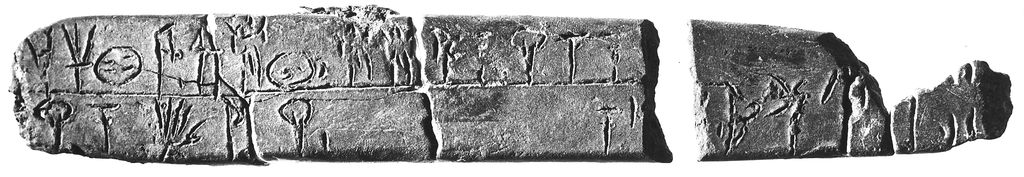
\includegraphics[width=0.7\textwidth]{Images/4901.png} % Adjust width and filename
    \caption{Picture of the original document PY Eb 895+906.}
    \label{fig:example1}
  \end{figure}

  \item \textbf{PY Ta 711}: This fragment is very short as well. It is excerpted from a longer document, whose translation will be fully evaluated in Section \ref{sec:translations}.
  However, it also contains a subordinate clause, introduced here by a particle.
  Moreover, it underscores the importance of grammatical and syntactic analysis, as the subject and the object of the sentence exhibit overlapping inflectional endings. \\
  \textbf{Linear B original}: \textlinb{\Bo\Bwi\Bde} \textlinb{\Bpu\Bke\Bqi\Bri} \textlinb{\Bo\Bte} \textlinb{\Bwa\Bna\Bka} \textlinb{\Bte\Bke} \textlinb{\Bau\Bke\Bwa} \textlinb{\Bda\Bmo\Bko\Bro}\\
  \textbf{Linear B text}: o-wi-de phu-ke-qi-ri o-te wa-na-ka te-ke au-ke-wa da-mo-ko-ro \\
  \textbf{Greek translation}: \textgreek{ὀ-εἶδε Φυγεκλής ὅτε ἄναξ θῆκε Αὐγέαν δάμοκλον} \\
  \textbf{English translation}: Phygekles witnessed when the king appointed Augeus as damoklos. \\

  \begin{figure}[H]
    \centering
    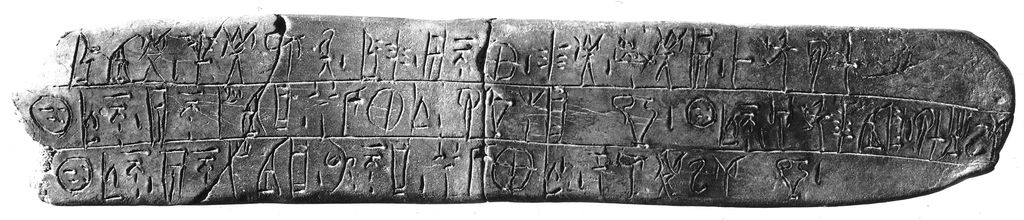
\includegraphics[width=0.8\textwidth]{Images/5350.png} % Adjust width and filename
    \caption{Picture of the original document PY Ta 711.}
    \label{fig:example2}
  \end{figure}

  \item \textbf{PY Ae 303}: This very brief document, like the previous two, illustrates long-distance agreement: the attributive adjective and the noun it modifies stand far apart in the line.
This word-order freedom is common in Ancient Greek and underscores why careful grammatical and logical analysis is essential. \\
  \textbf{Linear B original}: \textlinb{\Bi\Bje\Bro\Bjo} \textlinb{\Bpu\Bro} \textlinb{\Bi\Bje\Bre\Bja} \textlinb{\Bdo\Be\Bra} \textlinb{\Be\Bne\Bka} \textlinb{\Bku\Bru\Bso\Bjo} \textlinb{\BPwoman} \textlinb{\BNx\BNiv}\\
  \textbf{Linear B text}: i-je-ro-jo pu-ro i-je-re-ja do-e-ra e-ne-ka ku-ru-so-jo MUL 14 \\
  \textbf{Greek translation}: \textgreek{Πύλος: ιερείας δούλαι ένεκα χρυσοίο ιεροίο ΓΥΝΗ 14} \\
  \textbf{English translation}: Pylos: slaves of the priestess for the sake of sacred gold, 14 women. \\

  \begin{figure}[H]
    \centering
    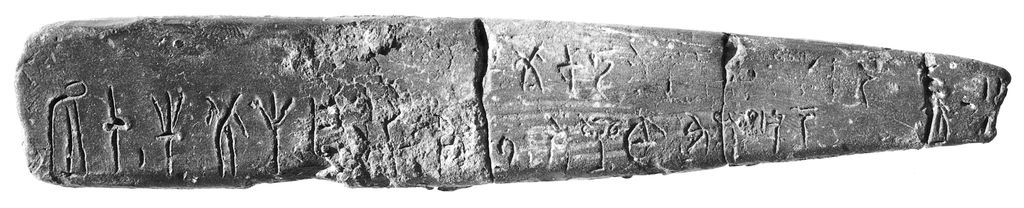
\includegraphics[width=0.7\textwidth]{Images/4684.png} % Adjust width and filename
    \caption{Picture of the original document PY Ae 303.}
    \label{fig:example3}
  \end{figure}

\end{enumerate}

\paragraph{Outputs}
The model is expected to output a JSON object with three fields:
\begin{itemize}
  \item \texttt{Ancient Greek}: the reconstructed Ancient Greek translation of the Linear B document.
  \item \texttt{English}: the English translation of the Linear B document.
  \item \texttt{Reasoning}: a detailed reasoning process, following the steps outlined in the task definition, explaining how the model arrived at its translations.
\end{itemize}

\section{Results} \label{sec:translations}
In this section, the outputs of the Translation Pipeline will be presented and compared with existing translations of the same documents, provided by Tselentis' lexicon \cite{tselentis}.

The parameters used for the LLM are the following: Gemini~2.5~Flash, with temperature 0.1, top-p 0.95, and top-k 0.4.

The evaluation will focus on the quality of the Ancient Greek reconstructions and the accuracy of the English translations.
Moreover, errors will be analyzed and the reasoning provided by the model will be assessed to understand the possible causes of mistakes.
A small sample of documents will not be assessed, as it was used as examples in the prompt (see Section \ref{sec:final-prompt}).

\subsection{Evaluated Documents}
The documents selected for evaluation are the following:
\begin{enumerate}[label=(\roman*)]
\item PY Ta 711
\item KN Ra 1540
\item PY Jn 310
\item PY Jn 829
\item KN So 4439
\item KN Sd 4404
\item PY An 657
\item PY TA 641
\item PY Er 312
\item KN Fp 1+31
\item PY Ab 573
\item PY Un 718
\end{enumerate}

The fragments of the documents whose translations were provided by Tselentis are highlighted in \emph{italics}.

\subsubsection{PY Ta 711}
This document was already presented as part of the examples in the prompt to the LLM.
However, only the first fragment was used as an example, while the rest of the document was reserved for evaluation. \\
\textbf{Linear B text}: \textit{o-wi-de phu-ke-qi-ri o-te wa-na-ka te-ke au-ke-wa da-mo-ko-ro} qe-ra-na wa-na-se-wi-ja qo-u-ka-ra ko-ki-re-ja *204VAS 1 qe-ra-na a-mo-te-wi-ja ko-ro-no-we-sa qe-ra-na wa-na-se-wi-ja ku-na-ja qo-u-ka-ra 1 to-qi-de-we-sa *204VAS 1 \\
\textbf{Greek translation}: \textgreek{ὀ-εἶδε Φυγεκλής ὅτε ἄναξ θῆκε Αὐγέαν δάμοκλον. κερανα ϝανασεϝια βουκαρα κοχλιρεια ΣΚΕΥΟΣ 1. κερανα αρμοθηϝια κορωνοϝέσσα. κερανα ϝανασεϝια γυναια βουκαρα 1. τροπιδϝέσσα ΣΚΕΥΟΣ 1.} \\
\textbf{English translation}: Phygekles witnessed when the king appointed Augeus as damoklos. A royal, ox-head-shaped, spiral-decorated krater (vessel): 1. A krater with fittings, with a handle. A royal, female, ox-head-shaped krater: 1. A spiral-designed vessel: 1.

\paragraph{Analysis.}
After the first narrative clause, the document lists four types of vessels.
The LLM correctly reconstructs the context and provides a meaningful and coherent translation.

Allow me to analyze the four vessel descriptions in detail:
\begin{itemize}
\item The word \textlinb{\Bqe\Bra\Bna} (qe-ra-na) is correctly identified as a noun, and the LLM selects the Ancient Greek cognate \textgreek{κερανα}.
However, the expected form would definitely be \textgreek{κέρνα}, the nominative/accusative plural of \textgreek{κέρνος}, which is used in Ancient Greek to denote a sacred vessel.
\item The word \textlinb{\Bwa\Bna\Bse\Bwi\Bja} (wa-na-se-wi-ja) is correctly identified as an adjective, and the LLM selects an Ancient Greek form that closely echoes the original Linear B word: \textgreek{ϝανασεϝια}, rather than the Ancient Greek \textgreek{αναξια}.
Other adjectives referring to this vessel are \textlinb{\Bqo\Bu\Bka\Bra} (qo-u-ka-ra, "ox-head shaped") and \textlinb{\Bko\Bi\Bre\Bja} (ko-ki-re-ja, "spiral-decorated").
The first is associated with a synthetic compound Ancient Greek form composed of \textgreek{βους} "ox" and \textgreek{καρα} "head", while the second is translated as \textgreek{κοχλιρεια}, an adjective derived from \textgreek{κοχλος}, "spiral-shaped shell", sharing the root with Ancient Greek \textgreek{κοχλιοειδης/κοκλιωδης}.
\item The following vessel is associated with the adjectives \textlinb{\Bko\Bro\Bno\Bwe\Bsa} (ko-ro-no-we-sa), meaning the krater is provided with handles (from Ancient Greek \textgreek{κορωνη}), and \textlinb{\Ba\Bmo\Bte\Bwi\Bja} (a-mo-te-wi-ja), linked to the concept of "fittings" or chariot-related terms (from Ancient Greek \textgreek{αρμος} "joint" and \textgreek{αρμα} "chariot"), even though no fully satisfactory Greek correspondence can be found.
\item The third vessel is again described as royal and ox-head shaped, but the third adjective is \textlinb{\Bku\Bna\Bja} (ku-na-ja), from Ancient Greek \textgreek{γυναια}, "womanly".
\item The last vessel is described as \textlinb{\Bto\Bqi\Bde\Bwe\Bsa} (to-qi-de-we-sa), "spiral-designed", from Ancient Greek \textgreek{τροπιδϝέσσα}, derived from \textgreek{τροπις}, which actually means "keel", and whose connection to spirals is only indirect through the notion of turning or curving, but is also confirmed by Tselentis' lexicon \cite{tselentis}.
\end{itemize}
Overall, the LLM's English translation is quite accurate, while the Ancient Greek reconstruction still retains Linear B features.

Here I report an improved version of the Greek translation, highlighting in red the adjustments. For the English translation, no changes are needed. \\
\textbf{Greek translation}: \textcolor{red}{\textgreek{οἶδε}} \textgreek{Φυγεκλής ὅτε ἄναξ θῆκε Αὐγέαν δάμοκλον.} \textcolor{red}{\textgreek{κέρνα ἀναξία}} \textgreek{βουκάρα} \textcolor{red}{\textgreek{κοχλιοειδή}} \textgreek{ΣΚΕΥΟΣ 1.} \textcolor{red}{\textgreek{κέρνα}} \textgreek{αρμοθήϝια κορωνοϝέσσα}. \textcolor{red}{\textgreek{κέρνα ἀναξία}} \textgreek{γυναίκα βουκάρα 1. τροπιδϝέσσα ΣΚΕΥΟΣ 1.}

The picture of this document is shown in Figure \ref{fig:example2}.

\subsubsection{KN Ra 1540}
This document is a very short inventory entry of a single item: swords. \\
\textbf{Linear B text}: \textit{to-sa pa-ka-na PUG 50} \\
\textbf{Greek translation}: \textgreek{τόσα φάσγανα ΦΑΣΓΑΝΑ 50.} \\
\textbf{English translation}: So many swords: 50 SWORDS.
\paragraph{Analysis.}
In this case, the LLM correctly reconstructs the whole document, due to its simplicity.
The words \textlinb{\Bto\Bsa} (to-sa) and \textlinb{\Bpa\Bka\Bna} (pa-ka-na) are correctly identified as a quantifier and a noun, respectively.
They are translated into their corresponding Ancient Greek cognates: \textgreek{τόσα} and \textgreek{ϝάσγανα}, the accusative plural of \textgreek{ϝάσγανον}, "sword".
The English translation is also accurate, therefore no changes are needed.

\begin{figure}[H]
  \centering
  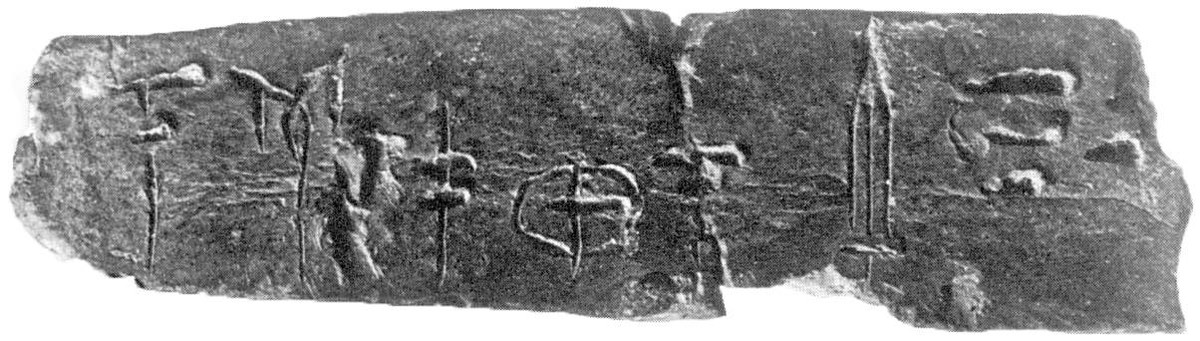
\includegraphics[width=0.7\textwidth]{Images/250.png} % Adjust width and filename
  \caption{Picture of the original document KN Ra 1540.}
  \label{fig:doc2}
\end{figure}

\subsubsection{PY Jn 310} \label{doc:pyjn310}
Tselentis provides a translation for only a fragment of this document, which is quite long.
However, the LLM appears able to handle the entire text well, thanks to its repetitive structure. \\
\textbf{Linear B text}: a-ke-re-wa [...] ka-ke-we ta-ra-si-ja e-ko-te ti-qa-jo AES M 1 N 2 qe-ta-wo AES M 1 N 2 ai-so-ni-jo AES M 1 N 2 ta-mi-je-u AES M 1 N 2 e-u-ru-wo-ta AES M 1 N 2 e-u-do-no AES M 1 N 2 po-ro-u-te-u AES M 1 N 2 wi-du-wa-ko AES M 1 N 2 to-so-de a-ta-ra-si-jo ka-ke-we [...] pa-qo-si-jo 1 ke-we-to 1 [...] 1 [...] pe-ta-ro 1 to-so-de do-e-ro ke-we-to-jo 1 i-wa-ka-o 1 pa-qo-si-jo-jo 1 po-ro-u-te-wo 1 a [...] \textit{po-ti-ni-ja-we-jo ka-ke-we ta-ra-si-ja e-ko-te} i-ma-di-jo [...] AES M 3 tu-ke-ne-u AES M 3 AES M 3 i-wa-ka AES M 3 a-ta-ra-si-jo phu-si-ja-ko 1 \\
\textbf{Greek translation}: \textgreek{Ἀγρεϝα [...] χαλκεϝες ταλανσία ἔχοντες: Τιθαιος ΧΑΛΚΟΣ M 1 N 2, Κεταϝος ΧΑΛΚΟΣ M 1 N 2, Αἰσώνιος ΧΑΛΚΟΣ M 1 N 2, Ταμιεύς ΧΑΛΚΟΣ M 1 N 2, Εὐρυϝότας ΧΑΛΚΟΣ M 1 N 2, Εὔδονος ΧΑΛΚΟΣ M 1 N 2, Πλουτεύς ΧΑΛΚΟΣ M 1 N 2, Ϝιδυϝακος ΧΑΛΚΟΣ M 1 N 2. Τόσοςδε ἀταλανσίοι χαλκεϝες [...]: Παμφίσιος 1, Κηϝετος 1, [...] 1, [...] 1, Πέταλος 1. Τόσοςδε δοῦλοι: Κηϝετοιο 1, Ἰϝακαο 1, Παμφισίοιο 1, Πλουτέϝος 1. Ἀ [...] Ποτνιάϝειοι χαλκεϝες ταλανσία ἔχοντες: Ἱμαδιος [...] ΧΑΛΚΟΣ M 3, Τυχενεύς ΧΑΛΚΟΣ M 3, ΧΑΛΚΟΣ M 3, Ἰϝακα ΧΑΛΚΟΣ M 3. Ἀταλανσίοι: Φυσίαρχος 1.} \\
\textbf{English translation}: Agrewa: [...] bronze-smiths having allotment: Tithaios: BRONZE M 1 N 2, Ketawo: BRONZE M 1 N 2, Aisonios: BRONZE M 1 N 2, Tamieus: BRONZE M 1 N 2, Eurywotas: BRONZE M 1 N 2, Eudonos: BRONZE M 1 N 2, Plouteus: BRONZE M 1 N 2, Widuwako: BRONZE M 1 N 2. Total bronze-smiths without allotment [...]: Pamphisios 1, Kewetos 1, [...] 1, [...] 1, Petalos 1. Total slaves: Of Kewetos 1, Of Iwaka 1, Of Pamphisios 1, Of Plouteus 1. A [...] Potnia-related bronze-smiths having allotment: Himadios [...] BRONZE M 3, Tucheneus: BRONZE M 3, BRONZE M 3, Iwaka: BRONZE M 3. Without allotment: Physiarchos 1.

\paragraph{Analysis.}
This document is an administrative record from the site of Pylos, listing bronze-smiths, their allotments of bronze, and associated personnel (slaves).
It is structured into several sections based on the status and affiliation of the craftsmen.
Most words occurring in the document are proper nouns, for which the Ancient Greek correspondence is a simple transliteration.
The most notable common words are:
\begin{itemize}
\item \textlinb{\Bka\Bke\Bwe} (ka-ke-we), "bronze-smith", from Ancient Greek \textgreek{χαλκεύς}, correctly identified as a noun by the LLM and transliterated in a form preserving the digamma (\textgreek{χαλκεϝες} rather than \textgreek{χαλκεῖς}).
\item \textlinb{\Bta\Bra\Bsi\Bja} (ta-ra-si-ja), "allotment", from Ancient Greek \textgreek{ταλανσία}, also correctly identified as a noun.
It shares its root with \textgreek{τάλαντον}, "talent", a unit of weight (and later currency), with the sense of "allotment" deriving from a weight of metal assigned to a worker.
\item \textlinb{\Be\Bko\Bte} (e-ko-te), "having", from Ancient Greek \textgreek{ἔχοντες}, the nominative plural masculine present active participle of \textgreek{ἔχω}, "to have".
Another straightforward form is \textlinb{\Bdo\Be\Bro} (do-e-ro), from Ancient Greek \textgreek{δοῦλοι}, the nominative plural masculine of \textgreek{δοῦλος}, "slave".
\item Both \textlinb{\Bto\Bso\Bde} (to-so-de) and \textlinb{\Ba\Bta\Bra\Bsi\Bjo} (a-ta-ra-si-jo) are interpreted as nominative plural adjectives referring to the bronze-smiths.
The former means "so many" or "total", from Ancient Greek \textgreek{τοσόσδε}, while the latter means "without allotment", from Ancient Greek \textgreek{ἀταλανσίος}, built from the negative prefix \textgreek{ἀ-} and \textgreek{ταλανσία}, "allotment".
\item The translation of \textlinb{\Bpo\Bti\Bni\Bja\Bwe\Bjo} (po-ti-ni-ja-we-jo) is problematic in this context.
While the LLM interprets it as a nominative plural associated with the bronze-smiths, Tselentis gives it a locative neuter value, linking it to the initial word \textlinb{\Ba\Bke\Bre\Bwa} (a-ke-re-wa), a toponym.
Accordingly, while the LLM's rendering remains vague, Tselentis' proposal is to read it as "at the place of Potnia", associating it with \textgreek{ποτνιάδειον}.
\end{itemize}

The LLM's English translation is quite accurate, although it reflects the issue with the word "po-ti-ni-ja-we-jo".
For both translations, I report an improved version below, highlighting in red the adjustments and in blue the actual mistakes. \\
\textbf{Greek translation}: \textgreek{Ἀγρεϝα [...]} \textcolor{red}{\textgreek{χαλκεῖς}} \textgreek{ταλανσία ἔχοντες: Τιθαιος ΧΑΛΚΟΣ M 1 N 2, Κεταϝος ΧΑΛΚΟΣ M 1 N 2, Αἰσώνιος ΧΑΛΚΟΣ M 1 N 2, Ταμιεύς ΧΑΛΚΟΣ M 1 N 2, Εὐρυϝότας ΧΑΛΚΟΣ M 1 N 2, Εὔδονος ΧΑΛΚΟΣ M 1 N 2, Πλουτεύς ΧΑΛΚΟΣ M 1 N 2, Ϝιδυϝακος ΧΑΛΚΟΣ M 1 N 2.} \textcolor{red}{\textgreek{Τοσοίδε}} \textgreek{ἀταλανσίοι} \textcolor{red}{\textgreek{χαλκεῖς}} \textgreek{[...]: Παμφίσιος 1, Κηϝετος 1, [...] 1, [...] 1, Πέταλος 1.} \textcolor{red}{\textgreek{Τοσοίδε}} \textgreek{δοῦλοι: Κηϝετοιο 1,} \textcolor{red}{\textgreek{Ἰϝακου}} \textgreek{1, Παμφισίοιο 1, Πλουτέϝος 1. Ἀ [...]} \textcolor{blue}{\textgreek{ποτνιάδειον}} \textcolor{red}{\textgreek{χαλκεῖς}} \textgreek{ταλανσία ἔχοντες: Ἱμαδιος [...] ΧΑΛΚΟΣ M 3, Τυχενεύς ΧΑΛΚΟΣ M 3, ΧΑΛΚΟΣ M 3,} \textcolor{red}{\textgreek{Ἰϝακας}} \textgreek{ΧΑΛΚΟΣ M 3. Ἀταλανσίοι: Φυσίαρχος 1.} \\
\textbf{English translation}: Agrewa: [...] bronze-smiths having allotment: Tithaios: BRONZE M 1 N 2, Ketawo: BRONZE M 1 N 2, Aisonios: BRONZE M 1 N 2, Tamieus: BRONZE M 1 N 2, Eurywotas: BRONZE M 1 N 2, Eudonos: BRONZE M 1 N 2, Plouteus: BRONZE M 1 N 2, Widuwako: BRONZE M 1 N 2. Total bronze-smiths without allotment [...]: Pamphisios 1, Kewetos 1, [...] 1, [...] 1, Petalos 1. Total slaves: Of Kewetos 1, Of \textcolor{red}{Iwakas} 1, Of Pamphisios 1, Of Plouteus 1. A [...] \textcolor{blue}{At the place of Potnia}: bronze-smiths having allotment: Himadios [...] BRONZE M 3, Tucheneus: BRONZE M 3, BRONZE M 3, \textcolor{red}{Iwakas}: BRONZE M 3. Without allotment: Physiarchos 1.

\begin{figure}[H]
  \centering
  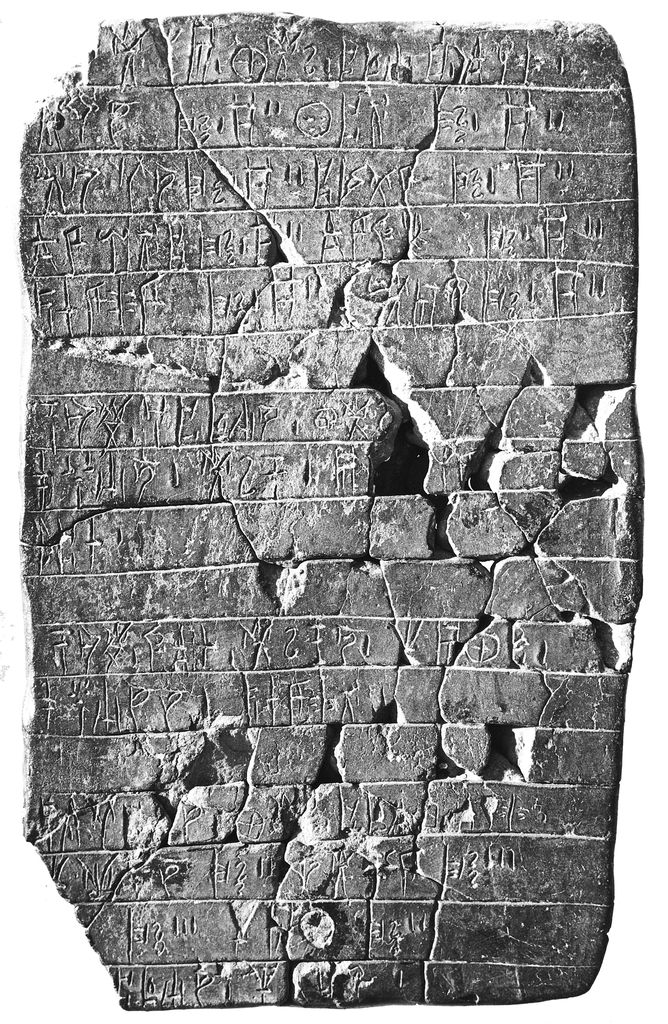
\includegraphics[width=0.55\textwidth]{Images/5057.png} % Adjust width and filename
  \caption{Picture of the original document PY Jn 310.}
  \label{fig:doc3}
\end{figure}

\subsubsection{PY Jn 829}
This document records the quantities of bronze collected for a temple and for the production of arrows.
The opening clause names the givers and states the purpose of the collection.
The remainder lists the amounts of bronze associated with various mayors and deputy mayors.
Because the closing portion is long and highly repetitive, I excluded it from the analysis.
Tselentis' translation covers only part of the opening sentence. \\
\textbf{Linear B text}: jo-do-so-si ko-re-te-re du-ma-te-qe po-ro-ko-re-te-re-qe ka-ra-wi-po-ro-qe o-pi-su-ko-qe o-pi-ka-pe-e-we-qe \textit{ka-ko na-wi-jo pa-ta-jo-i-qe e-ke-si-qe ai-ka-sa-ma} pi-*82 ko-re-te AES M 2 po-ro-ko-re-te AES N 3 me-ta-pa ko-re-te AES M 2 po-ro-ko-re-te AES N 3 [...] \\
\textbf{Greek translation}: \textgreek{Ὡς δώσουσι κορητῆρες δῠμᾶτές τε προκορητῆρές τε κλαϝιφόροί τε ὀπίσυκοί τε ὀπικαπεῆϝές τε χαλκόν ναϝίον, παλταίοις τε ἔχεσσι τε αἰχμάς. Πίσαϝι: κορητήρ ΧΑΛΚΟΣ M 2, προκορητήρ ΧΑΛΚΟΣ N 3. Μετάπα: κορητήρ ΧΑΛΚΟΣ M 2, προκορητήρ ΧΑΛΚΟΣ N 3.} \\
\textbf{English translation}: Thus will give the mayors and magistrates and deputy mayors and key-bearers and overseers of figs and overseers of digging, temple bronze, and spearheads for the javelin-men and for the spears. Pisa: mayor, bronze M 2, deputy mayor, bronze N 3. Metapa: mayor, bronze M 2, deputy mayor, bronze N 3. 

\paragraph{Analysis.}
The first part of the document lists the officials responsible for collecting bronze for a temple and for the production of arrows.
The LLM correctly identifies the main terms in this section, but it struggles with a few specific titles.
In the second part, the LLM correctly recognizes the place names and the officials; however, it is uncertain whether these officials are the collectors or the recipients of the bronze.
Given the usual structure of Linear B documents, they are more likely the collectors, since the introductory clause states that the bronze will be given by the officials.

The main terms in the first part of the document are:
\begin{itemize}
  \item \textlinb{\Bjo\Bdo\Bso\Bi\Bsi} (jo-do-so-si), "thus will give", from Ancient Greek \textgreek{ὡς δώσουσι}, the 3rd person plural future active indicative of \textgreek{δίδωμι} "to give".
  \item A series of Mycenaean official titles, correctly treated as nouns by the LLM. The most frequent here are \textlinb{\Bko\Be\Bre\Bte\Bre} (ko-re-te-re) "mayors" and \textlinb{\Bpo\Bro\Bko\Be\Bre\Bte\Bre} (po-ro-ko-re-te-re) "deputy mayors".
  Although the latter is transparently the former with a \textgreek{προ-} prefix, I find no fully satisfactory classical Greek equivalent beyond a transliteration.
  \item Additional titles include \textlinb{\Bdu\Bma\Bte} (du-ma-te) "magistrates/dāmos officials", linked by Tselentis to \textgreek{δῆμος} "people"; \textlinb{\Bka\Bra\Bwi\Bpo\Bro} (ka-ra-wi-po-ro) "key-bearers", from \textgreek{κλείς} "key" and \textgreek{φέρω} "carry/bear"; \textlinb{\Bo\Bpi\Bsu\Bko} (o-pi-su-ko) "overseers of figs", from \textgreek{ἐπί} "over" and \textgreek{σῦκον} "fig"; and \textlinb{\Bo\Bpi\Bka\Bpe\Be\Bwe} (o-pi-ka-pe-e-we) "overseers of digging", from \textgreek{σκάπτω} "to dig".
  \item The first object of the collection is bronze destined for a temple: \textlinb{\Bka\Bko} (ka-ko) "bronze", from \textgreek{χαλκόν}, and its adjective \textlinb{\Bna\Bwi\Bjo} (na-wi-jo) "temple-/sacral-", from \textgreek{ναίος} "of a temple".
  \item The second object consists of spearheads for javelins and for spears.
  These are expressed by \textlinb{\Baiii\Bka\Bsa\Bma} (ai-ka-sa-ma) "spearheads", from \textgreek{αἰχμή} (used here in the plural accusative), and by \textlinb{\Bpa\Bta\Bjo\Bi} (pa-ta-jo-i) "for javelins", from \textgreek{παλτόν}, and \textlinb{\Be\Bke\Bsi} (e-ke-si) "for the spears", from \textgreek{ἔγχος} (dative plural).
  The LLM, however, misinterpreted \textit{pa-ta-jo-i}, treating it as an adjective ("javelin-using") rather than as the noun "javelins," likely due to a misclassification.  \item The first toponym \textlinb{\Bpi\Bswa} (pi-*82) contains an uncertain syllabogram whose phonetic value is commonly taken to be "swa".
  \item The remainder of the tablet simply enumerates toponyms together with the quantities of bronze associated with each \textit{ko-re-te} (mayor) and \textit{po-ro-ko-re-te} (deputy mayor).
\end{itemize}

Here I report an improved version of the translations, highlighting in red the adjustments. \\
\textbf{Greek translation}: \textgreek{Ὡς δώσουσι κορητῆρες δῠμᾶτές τε προκορητῆρές τε κλαϝιφόροί τε} \textcolor{red}{\textgreek{ἐπισυκοί}} \textgreek{τε} \textcolor{red}{\textgreek{ἐπισκαπηϝές}} \textgreek{τε χαλκόν ναϝίον,} \textcolor{blue}{\textgreek{παλτοῖς}} \textgreek{τε} \textcolor{red}{\textgreek{ἔγχεσι}} \textgreek{τε αἰχμάς.} \textcolor{red}{\textgreek{Πίσϝα:}} \textgreek{κορητήρ ΧΑΛΚΟΣ M 2, προκορητήρ ΧΑΛΚΟΣ N 3. Μετάπα: κορητήρ ΧΑΛΚΟΣ M 2, προκορητήρ ΧΑΛΚΟΣ N 3.} \\
\textbf{English translation}: Thus will give the mayors and magistrates and deputy mayors and key-bearers and overseers of figs and overseers of digging, bronze \textcolor{red}{for the temple}, and spearheads for the \textcolor{blue}{javelins} and for the spears. \textcolor{red}{Piswa}: mayor, bronze M 2, deputy mayor, bronze N 3. Metapa: mayor, bronze M 2, deputy mayor, bronze N 3.

\begin{figure}[H]
  \centering
  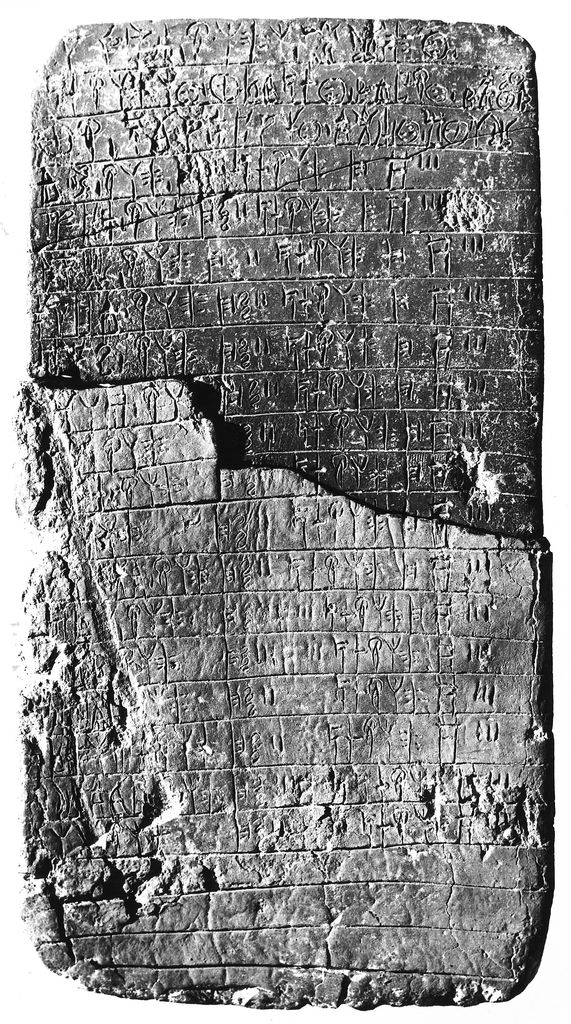
\includegraphics[width=0.35\textwidth]{Images/5072.png} % Adjust width and filename
  \caption{Picture of the original document PY Jn 829.}
  \label{fig:doc4}
\end{figure}

\subsubsection{KN So 4439} \label{doc:knso4439}
This very short document is an inventory of wheels.
Despite its brevity, it is actually one of the most challenging documents due to the presence of misleading words.
Tselentis provides the translation for the entire document. \\
\textbf{Linear B text}: \textit{a-mo-ta e-ri-ka te-mi-dwe-ta ROTA ZE 3 MO ROTA 1} \\
\textbf{Greek translation}: \textgreek{ἁρμότα ἑλίκαι τερμιδϝέντα: τροχοί ζεύγη 3, μόνος τροχός 1.} \\
\textbf{English translation}: Chariot fittings, willow (wood), rimmed: 3 pairs of wheels, 1 single wheel.

\paragraph{Analysis.}
The analysis of this document is particularly important, as it highlights the challenges posed by certain words that can easily mislead the LLM.
The main terms in this document are:
\begin{itemize}
  \item \textlinb{\Ba\Bmo\Bta} (a-mo-ta), "wheels/chariot", from Ancient Greek \textgreek{ἅρμα}, is the nominative plural and subject of the sentence.
  Despite its original meaning as "wheel", in classical Ancient Greek it came to denote the entire chariot.
  \item \textlinb{\Be\Bri\Bka} (e-ri-ka), "willow tree", from Ancient Greek \textgreek{ἑλικτός}, is here used as an adjective to describe the material of the wheels.
  However, the LLM misinterprets it as a noun, translating it as "willow". Moreover, its connection to the concept of "willow" is attested in Linear B, while in classical Ancient Greek \textgreek{ἑλικτός} means "twisted" or "curved".
  \item \textlinb{\Bte\Bmi\Bdwe\Bta} (te-mi-dwe-ta), "rimmed", from Ancient Greek \textgreek{τερμιόεις}, is correctly identified as an adjective by the LLM.
\end{itemize}
The LLM's English translation fails to capture the full meaning of the document, as it misunderstands the subject of the sentence and misinterprets the adjective referring to the material of the wheels.
Here I report an improved version of the translations, highlighting in red the adjustments and in blue the actual mistakes. \\
\textbf{Greek translation}: \textcolor{red}{\textgreek{ἅρματα}} \textcolor{blue}{\textgreek{ἑλικά}} \textcolor{red}{\textgreek{τερμιοέντα}}\textgreek{: τροχοί ζεύγη 3, μόνος τροχός 1.} \\ 
\textbf{English translation}: \textcolor{blue}{Wheels made of willow tree}, rimmed: 3 pairs of wheels, 1 single wheel.

\begin{figure}[H]
  \centering
  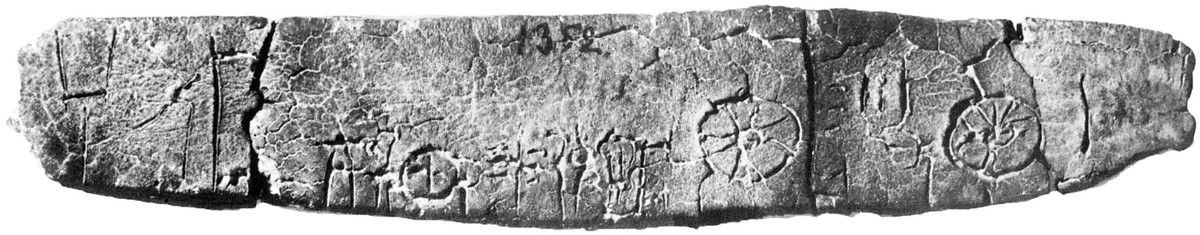
\includegraphics[width=0.7\textwidth]{Images/568.png} % Adjust width and filename
  \caption{Picture of the original document KN So 4439.}
  \label{fig:doc5}
\end{figure}

\subsubsection{KN Sd 4404}
This document is another inventory, this time for chariots.
Due to its fragmentary state, reconstructing its content is challenging.
Tselentis provides a translation for only the last fragment of the document. \\
\textbf{Linear B text}: jo [...] i-qo-e-qe wi-ri-ni-jo o-po-qo ke-ra-ja-pi o-pi-i-ja-pi CUR [...] \textit{i-qi-ja [...] ku-do-ni-ja mi-to-we-sa-e a-ra-ro-mo-te-me-na} po-ni-ki-ja BIG 1 \\
\textbf{Greek translation}: \textgreek{[...], ἱππο-ε-κες τε ϝίρινιοι ὀπωπω κεραίαφι ὀπίαιφι ΔΙΦΡΟΣ. [...] ἱππία Κυδωνία μιλτόϝεσσα ἀραρμοτhεμένη φοινικία ΔΙΦΡΟΣ 1.} \\
\textbf{English translation}: [...], and horse-equipped (parts), leathern eye-guards, with horn-like parts, with reins, a chariot. [...] A Cydonian, red-painted, fitted, red-dyed chariot: 1 chariot.

\paragraph{Analysis.}
Overall, the LLM performs well in recognizing the main words in the document, despite its fragmentary condition.
The main terms in this document are:
\begin{itemize}
  \item \textlinb{\Bi\Bqo\Be\Bqe} (i-qo-e-qe), which is linked to \textgreek{ἵππος} "horse". 
  It presents a strange \textit{-e} ending, and is interpreted as "horse-equipped parts", despite the fact that \textit{-qe} is usually a conjunction meaning "and".
  The peculiar ending might be dual ending, but this is only my speculation.
  \item \textlinb{\Bwi\Bri\Bni\Bo} (wi-ri-ni-jo) derives from \textgreek{ῥινός}, "leather", and it is an adjective associated with \textlinb{\Bo\Bpo\Bqo} (o-po-qo), "eye-guards", from \textgreek{ἐπί} and the root \textgreek{ὀπ-}, linked to sight, as in \textgreek{ὄψις}, "sight".
  \item \textgreek{κεραίαφι} (ke-ra-ja-pi) and \textgreek{ὀπίαιφι} (o-pi-i-ja-pi) are both in the instrumental terms, as indicated by the suffix \textit{-pi}, and mean "with horn-like parts" and "with reins".
  The former comes from Ancient Greek \textgreek{κέρας} "horn", while the latter has an uncertain etymology, possibly linked to \textgreek{ἡνία} "reins", combined with the \textgreek{ἐπί} prefix.
  \item \textlinb{\Bi\Bqi\Ba} (i-qi-ja) is the word for "chariot", from Ancient Greek \textgreek{ἵππια}, adjective related to \textgreek{ἵππος}, "horse".
  \item Three adjectives describe the chariot: \textlinb{\Bku\Bdo\Bni\Ba} (ku-do-ni-ja) is the toponym "Cydonia", from the ancient city of Cydonia in Crete.
  \textlinb{\Bmi\Bto\Bwe\Bsa\Be} (mi-to-we-sa-e) and \textlinb{\Bpo\Bni\Bki\Bja} (po-ni-ki-ja) mean "purple red-painted", from Ancient Greek \textgreek{μιλτός}, "red ochre" and \textgreek{φοινίκιος}, "phoenician", respectively. 
  \textlinb{\Ba\Bra\Bro\Bmo\Bte\Bme\Bna} (a-ra-ro-mo-te-me-na) is the passive participle of \textgreek{ἀρμόζω}, and means "fitted/assembled".
\end{itemize}
I provide an improved version of the translations below, highlighting in red the adjustments. \\
\textbf{Greek translation}: \textgreek{[...],} \textcolor{red}{\textgreek{ἱππω τε ϝρινιοι}} \textgreek{ὀπωπω κεραίαφι ὀπίαιφι ΔΙΦΡΟΣ. [...] ἱππία Κυδωνία μιλτόϝεσσα ἀραρμοτhεμένη φοινικία ΔΙΦΡΟΣ 1.} \\
\textbf{English translation}: [...], \textcolor{red}{(equipped with) two horses, with} leathern eye-guards, with horn-like parts, with reins, a chariot. [...] A Cydonian, \textcolor{blue}{purple red-painted}, \textcolor{red}{assembled}, chariot: 1 chariot.

\begin{figure}[H]
  \centering
  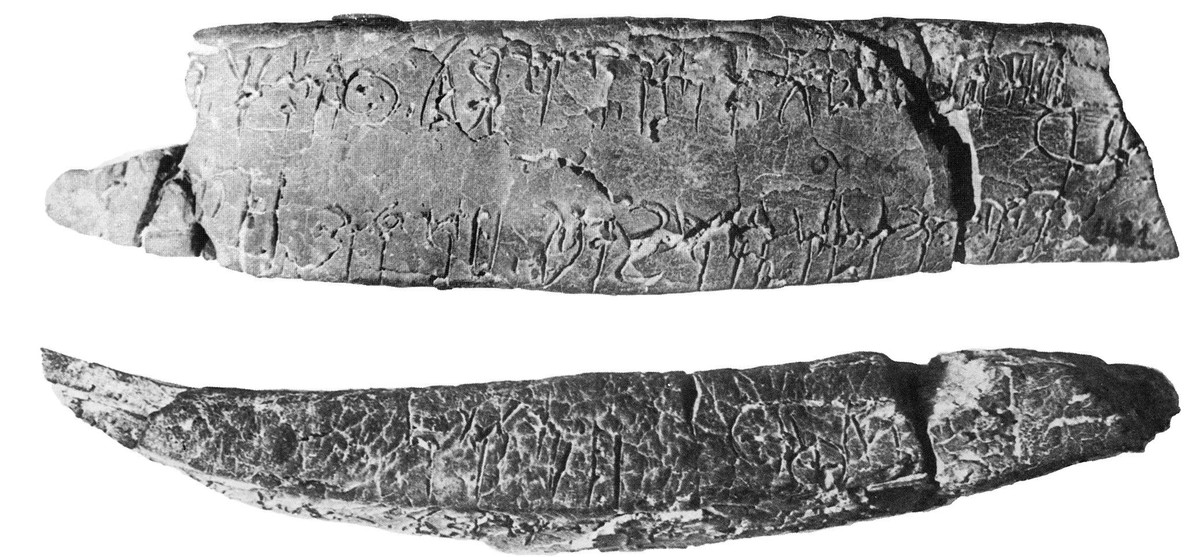
\includegraphics[width=0.7\textwidth]{Images/454.png} % Adjust width and filename
  \caption{Picture of the original document KN Sd 4404.}
  \label{fig:doc6}
\end{figure}

\subsubsection{PY An 657} \label{doc:pyan657}
This document lists various groups of guards and soldiers, together with their numbers, the names of their leaders, and the place of deployment.
Tselentis provides a translation for a small portion of the text containing the name of an "epetas". \\

\textbf{Linear B text}: o-u-ru-to o-pi-ha-ra e-pi-ko-wo ma-re-wo o-ka o-wi-to-no a-pe-ri-ta-wo o-re-ta e-te-wa ko-ki-jo su-we-ro-wi-jo o-wi-ti-ni-jo o-ka-rai VIR 50 ne-da-wa-ta-o o-ka e-ke-me-de a-pi-je-ta ma-ra-te-u ta-ni-ko ha-ru-wo-te ke-ki-de ku-pa-ri-si-jo VIR 20 ai-ta-re-u-si ku-pa-ri-si-jo ke-ki-de VIR 10 \textit{me-ta-qe pe-i e-qe-ta ke-ki-jo} a-e-ri-qo-ta e-ra-po ri-me-ne o-ka-ra o-wi-to-no VIR 30 ke-ki-de-qe a-phu-ka-ne VIR 20 me-ta-qe pe-i ai-ko-ta e-qe-ta \\
\textbf{Greek translation}: \textgreek{Οὖροι Ὀπίχαρα, ἐπίκουροι. Μαλέϝος ὀρχά Ὀϝιτνῶι. Ἀπερίταϝος, Ὀρέλτας, Ἐτέϝας, Κόκκιος, Συϝεροϝιος, Ὀϝιτίνιος. Ὀρχᾶραι: ἄνδρες 50. Νεδαϝάταο ὀρχά. Ἐχεμήδης, Ἀμφιγέτας, Μαλθεύς, Τάνικος. Ἁρυϝότει Κεκκίδες Κυπαρίσσιοι: ἄνδρες 20. Αἰθαλεῦσι Κυπαρίσσιοι Κεκκίδες: ἄνδρες 10. μετά τε σφεῖ ἑπέτας Κέρκιος, Ἀελιπότας, Ἔλαφος. Λιμένει Ὀρχάρα Ὀϝιτνῶι: ἄνδρες 30. Κεκκίδες τε Ἀφυγάνες: ἄνδρες 20. μετά τε σφεῖ Αἰκότας ἑπέτας.} \\
\textbf{English translation}: Guards at Opihara, auxiliaries. Maleus' company at Owitnos. Aperitawos, Orelas, Etewas, Kokkios, Suwerowios, Owitinios. Orcharai: 50 men. Nedawatas' company. Echemedes, Amphigetas, Maltheus, Tanikos. At Harywos, Kekkides Kyparissioi: 20 men. At Aithaleus, Kyparissioi Kekkides: 10 men. And with them, the follower Kerkios, Aelipotas, Elaphos. At Limen, Orchara at Owitnos: 30 men. And Kekkides Aphuganes: 20 men. And with them, Aikotas, the follower.

\paragraph{Analysis.}
Overall, the LLM performs well in recognizing the logical function of the words in the document, despite erroneously treating some of them as proper nouns.
Moreover, it recognizes ethnonyms, but simply transliterates them without attempting to interpret the places to which they relate.

The main terms in this document are:
\begin{itemize}
  \item \textlinb{\Bo\Bu\Bru\Bto} \textlinb{\Be\Bpi\Bko\Bwo} (o-u-ru-to e-pi-ko-wo), "auxiliary guards", from Ancient Greek \textgreek{οὖρος} "guardian" and \textgreek{ἐπίκουρος} "auxiliary".
  \item \textlinb{\Bo\Bpi\Ba2\Bra} (o-pi-ha-ra), is correctly recognized as a place name, but it probably means "at the coast", as also in Homer the term \textgreek{ἐφαλός} is attested, combining the prefix \textgreek{ἐπί} with \textgreek{ἅλς/ἁλός} "sea". 
  \item \textlinb{\Bo\Bka} (o-ka), "company/military unit", corresponds to Ancient Greek \textgreek{ἀρχή}.
  \item \textlinb{\Bo\Bwi\Bto\Bno} (o-wi-to-no), "Owitnos", is correctly identified as a toponym.
  \item \textlinb{\Bo\Bwi\Bto\Bni\Bjo} \textlinb{\Bo\Bwi\Bka\Braiii} (o-wi-ti-ni-jo o-ka-rai), are treated separately by the LLM, but in my opinion they are connected.
  Instead of a proper name, o-wi-ti-ni-jo is probably an ethnonym adjective meaning "of Owitnos", referred to o-ka-rai, which the LLM correctly identifies as a group of people, but not as an ethnic name ("Oihalai", from Tselentis lexicon).
  So they are both ethnonyms.
  \item \textlinb{\Bme\Bta\Bqe} \textlinb{\Bpe\Bi} (me-ta-qe pe-i), "and with them", from Ancient Greek \textgreek{μετά} "with", \textgreek{σφεῖς} "them".
  \item \textlinb{\Be\Bqe\Bta} (e-qe-ta) is a military title meaning "follower/attendant", from Ancient Greek \textgreek{ἑπέτας}.
  \item Other companies, deployed in other locations, are then listed in a similar manner.
  \item \textlinb{\Be\Bra\Bpo} \textlinb{\Bri\Bme\Bne} (e-ra-po ri-me-ne), is completely misinterpreted by the LLM.
  It should be interpreted as "the port of the deers", from Ancient Greek \textgreek{λιμήν} "port" and \textgreek{ἔλαφος} "deers", combined into \textgreek{ἐλάφων λιμένι}.
\end{itemize}

Overall, the high number of proper nouns, ethnonyms and toponyms and the varying structure of the sentences make the translation of this document challenging.

The last part of the document is not straightforward, as it presents two place names (\textit{o-ka-ra} and \textit{o-wi-to-no}) that are close and are assumed to be related, since they also appear together as ethnonyms.
However, I cannot be sure about the correctness of this choice.
Here I report an improved version of the translations, highlighting in red the adjustments and in blue the actual mistakes.
Beware that the last part of the document is uncertain. \\
\textbf{Greek translation}: \textgreek{Οὖροι} \textcolor{blue}{\textgreek{ἐφαλός}}\textgreek{, ἐπίκουροι. Μαλέϝος} \textcolor{red}{\textgreek{ἀρχή}} \textgreek{Ὀϝιτνῷ. Ἀπερίταϝος, Ὀρέλτας, Ἐτέϝας,} \textcolor{red}{\textgreek{Κόλκιος}}\textgreek{, Συϝεροϝιος.} \textcolor{blue}{\textgreek{Ὀϝιτίνιοι Οἰχαλεαι}}\textgreek{: ἄνδρες 50. Νεδαϝάταο} \textcolor{red}{\textgreek{ἀρχή}}\textgreek{. Ἐχεμήδης, Ἀμφιγέτας, Μαλθεύς, Τάνικος.} \textcolor{red}{\textgreek{Ἁρυϝόθεν Κελχίδες Κυπαρίσιοι}}\textgreek{: ἄνδρες 20. Αἰθαλεῦσι} \textcolor{red}{\textgreek{Κελχίδες Κυπαρίσιοι}}\textgreek{: ἄνδρες 10. μετά τε} \textcolor{red}{\textgreek{σφεῖς}} \textgreek{ἑπέτας Κέρκιος. Ἀελιπότας,} \textcolor{blue}{\textgreek{ἐλάφων λιμένι}} \textcolor{red}{\textgreek{Ὀιχαλᾳ}} \textgreek{Ὀϝιτνῷ: ἄνδρες 30.} \textcolor{red}{\textgreek{Κελχίδες}} \textgreek{τε Ἀφυγάνες: ἄνδρες 20. μετά τε} \textcolor{red}{\textgreek{σφεῖς}} \textgreek{Αἰκότας ἑπέτας.} \\
\textbf{English translation}: Guards at \textcolor{blue}{the coast}, auxiliaries. Maleus' company at Owitnos: Aperitawos, Orelas, Etewas, \textcolor{red}{Kolchios}, Suwerowios. \textcolor{blue}{(People) from Owitnos and Oichala}: 50 men. Nedawatas' company. Echemedes, Amphigetas, Maltheus, Tanikos. At Harywos, \textcolor{red}{(people) from Kelchis and Kyparisos}: 20 men. At Aithaleus, \textcolor{red}{(people) from Kelchis and Kyparisos}: 10 men. And with them, the \textcolor{red}{attendant} Kerkios. Aelipotas, \textcolor{blue}{at the deers' port} \textcolor{red}{in Oichala} at Owitnos: 30 men. \textcolor{red}{(People) from Kelchis and Aphy}: 20 men. And with them, Aikotas, the \textcolor{red}{attendant}.

\begin{figure}[H]
  \centering
  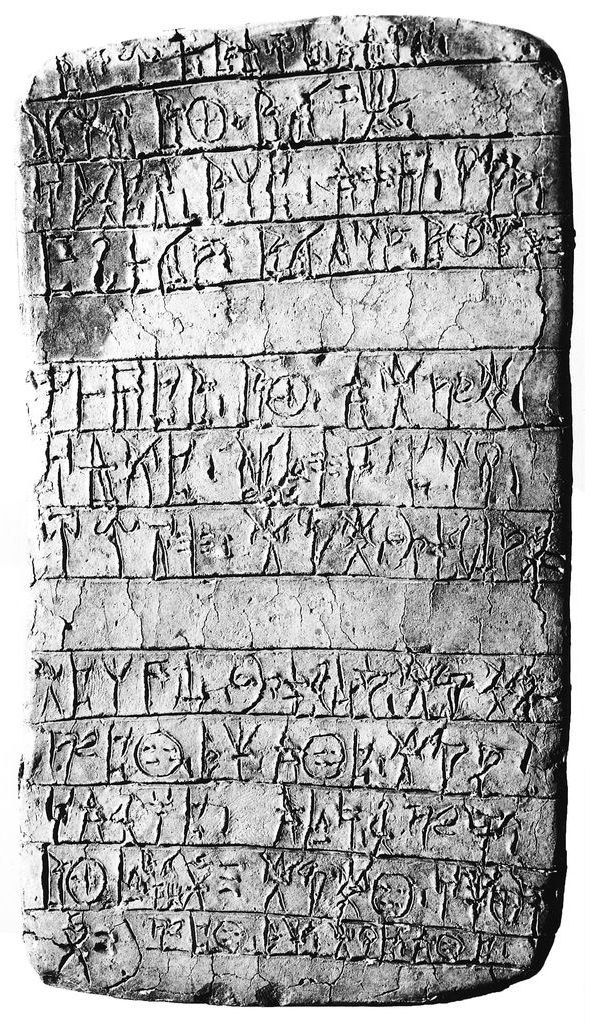
\includegraphics[width=0.4\textwidth]{Images/4726.png} % Adjust width and filename
  \caption{Picture of the original document PY An 657.}
  \label{fig:doc7}
\end{figure}

\subsubsection{PY TA 641} \label{doc:pyta641}
This document is a short inventory of vessels, in particular tripods and pithoi (large storage jars).
The translation provided by Tselentis covers the first portion of the document, while the rest is left untranslated. \\
\textbf{Linear B text}: \textit{ke-re-ha *201VAS [...] ti-ri-po-de ai-ke-u ke-re-si-jo we-ke *201VAS 2 ti-ri-po e-me po-de o-wo-we *201VAS 1 ti-ri-po ke-re-si-jo we-ke a-pu ke-ka-u-me-no} [...] qe-to *203VAS 3 di-pa me-zo-e qe-to-ro-we *202VAS 1 di-pa-e me-zo-e ti-ri-o-we-e *202VAS 2 di-pa me-wi-jo qe-to-ro-we *202VAS 1 di-pa me-wi-jo ti-ri-jo-we *202VAS 1 di-pa me-wi-jo a-no-we *202VAS 1 \\
\textbf{Greek translation}: \textgreek{Σκελέα *201VAS [...] Τρίποδες Αἰγεύς Κρήσιος ἔργε *201VAS 2. Τρίπους ἐν ποδεί ὄϝοϝεις *201VAS 1. Τρίπους Κρήσιος ἔργε ἀπὸ κεκαυμένος. Πίθοι *203VAS 3. Δέπας μεῖζον τετρόϝες *202VAS 1. Δέπαε μείζοε τριόϝεε *202VAS 2. Δέπας μεῖον τετρόϝes *202VAS 1. Δέπας μεῖον τριόϝes *202VAS 1. Δέπας μεῖον ἄνοϝον *202VAS 1.} \\
\textbf{English translation}: Tripod with legs [...] Two tripods, Aigeus, Cretan-made. One tripod, with one foot, one-handled. One tripod, Cretan-made, burnt off. Three jars. One larger, four-handled cup. Two larger, three-handled cups. One smaller, four-handled cup. One smaller, three-handled cup. One smaller, handleless cup.

\paragraph{Analysis.}
In this document, the main problem is the positioning of the first two words, which occur at the beginning of the document but should probably be appended to the end of the first line.
They were added at the top right of the first row, as the scribe likely ran out of space to complete the line.
The translation clearly inherits this misplacement.
A notable aspect of this fragment is the presence of the dual, attested when describing two cups.

The LLM correctly identifies the main words in the document
\begin{itemize}
  \item \textlinb{\Bke\Bre\Bre\Baii} (ke-re-ha), "legs", from Ancient Greek \textgreek{σκελέα}, is a noun, linked to the verb \textit{ke-ka-u-me-no}, specifying where the tripod is burnt.  
  \item \textlinb{\Bti\Bri\Bpo}[\textlinb{\Bde}] (ti-ri-po[-de]), \textlinb{\Bqe\Bto} (qe-to), and \textlinb{\Bdi\Bpa} (di-pa) are the Linear B words for \textgreek{τρίπους} "tripod", \textgreek{πίθος} "jar" and \textgreek{δέπας} "cup", respectively.
  \item \textlinb{\Ba\Bi\Bke\Bu} (ai-ke-u), "Aigeus", is correctly identified as a proper name, despite not being linked to anything precisely, like in Tselentis translation.
  \item \textlinb{\Bke\Bre\Bse\Bi\Bjo} \textlinb{\Bwe\Bke} (ke-re-si-jo we-ke), "Cretan-made", from Ancient Greek \textgreek{Κρήσιος} "Cretan" and \textgreek{ἔργον} "work", is an description linked to the tripods. 
  \item \textlinb{\Be\Bme} \textlinb{\Bpo\Bde} (e-me po-de), "with one foot", from Ancient Greek \textgreek{ἐνί ποδεί}, is another description linked to a tripod.
  It is interesting to note that the LLM correctly interprets \textit{e-me} as the numeral "one", even though it is misinterpreted in the analysis and in the translation.
  \item \textlinb{\Bo\Bwo\Bwe} (o-wo-we), \textlinb{\Bqe\Bto\Bro\Bwe} (qe-to-ro-we), \textlinb{\Bti\Bri\Bjo\Bwe} (ti-ri-o-we-e), and \textlinb{\Ba\Bo\Bno\Be} (a-no-we) are adjectives linked to the jars, meaning "one-handled", "four-handled", "three-handled", and "handleless", respectively.
  \item \textlinb{\Bke\Bka\Bu\Bme\Bno} (ke-ka-u-me-no), "burnt off", from the Ancient Greek verb \textgreek{καίω}, is a perfect passive participle linked to a tripod.
  \item \textlinb{\Bme\Bzo\Be} (me-zo-e) and \textlinb{\Bme\Bwi\Bjo} (me-wi-jo) are adjectives linked to the cups, meaning "larger" and "smaller" from Ancient Greek \textgreek{μείζων} and \textgreek{μείων}, respectively.
\end{itemize}

Here I report a refined version of both translations, adding the first two words at the end of the first line and highlighting in red the adjustments and in blue the mistakes. \\
\textbf{Greek translation}: \textgreek{Τρίποδες Αἰγεύς} \textcolor{red}{\textgreek{Κρήσιου ἔργου}} \textgreek{*201VAS 2. Τρίπους} \textgreek{ἐνί} \textgreek{ποδεί} \textcolor{red}{\textgreek{ὠτόϝεις}} \textgreek{*201VAS 1. Τρίπους} \textcolor{red}{\textgreek{Κρήσιου ἔργου}} \textgreek{κεκαυμένος} \textcolor{blue}{\textgreek{ἀπὸ σκελέα *201VAS}}\textgreek{. Πίθοι *203VAS 3. Δέπας μεῖζον} \textcolor{red}{\textgreek{τετραώτον}} \textgreek{*202VAS 1.} \textcolor{red}{\textgreek{Δέπα μείζονε τριώτω}} \textgreek{*202VAS 2. Δέπας μεῖον} \textcolor{red}{\textgreek{τετραώτον}} \textgreek{*202VAS 1. Δέπας μεῖον} \textcolor{red}{\textgreek{τριώτον}} \textgreek{*202VAS 1. Δέπας μεῖον} \textcolor{red}{\textgreek{ἀνώτον}} \textgreek{*202VAS 1.} \\
\textbf{English translation}: Two tripods, Aigeus, Cretan-made. One tripod, with one foot, one-handled. One tripod, Cretan-made, burnt off \textcolor{blue}{at the legs}. Three jars. One larger, four-handled cup. Two larger, three-handled cups. One smaller, four-handled cup. One smaller, three-handled cup. One smaller, handleless cup.


\begin{figure}[H]
  \centering
  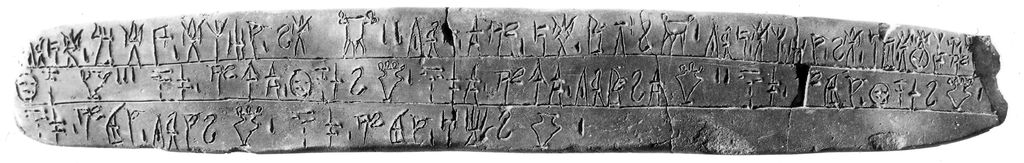
\includegraphics[width=0.7\textwidth]{Images/5344.png} % Adjust width and filename
  \caption{Picture of the original document PY TA 641.}
  \label{fig:doc8}
\end{figure}


\subsubsection{PY Er 312} \label{doc:pyer312}
This document lists various land holdings together with their grain quantities and associated personnel.
Tselentis provides a translation for the entire document.  \\
\textbf{Linear B text}: \textit{wa-na-ka-te-ro te-me-no to-so-jo pe-ma GRA 30 ra-wa-ke-si-jo te-me-no GRA 10 te-re-ta-o to-so pe-ma GRA 30 to-so-de te-re-ta VIR 3 wo-ro-ki-jo-ne-jo e-re-mo to-so-jo pe-ma GRA 6} \\
\textbf{Greek translation}: \textgreek{ϝανακτέρον τέμενος: τοσοῖο σπέρματος ΓΡΑ 30. λαϝαγεσίοιο τέμενος: ΓΡΑ 10. τελεσταῶν τόσον σπέρμα: ΓΡΑ 30. τοσόνδε τελεσταί: ΑΝΗΡ 3. ϝοργιονείοιο ἔρημον: τοσοῖο σπέρματος ΓΡΑ 6.} \\
\textbf{English translation}: Royal temenos: of so much grain, GRA 30. Temenos of the lawagetas: GRA 10. Of the telestai, so much grain: GRA 30. And so many telestai: 3 men. Fallow land of Worgion: of so much grain, GRA 6.

\paragraph{Analysis.} The LLM performs well in recognizing all the words in the document.
It also recognizes the logograms in its analysis, although it simply transliterates them in the translation.
The translation is accurate overall, helped by the clear, list-like structure of the entries.
The main terms are:
\begin{itemize}
  \item \textlinb{\Bte\Bme\Bno} (te-me-no), "temenos", from Ancient Greek \textgreek{τέμενος}. Its usual meaning is "sacred precinct", but here it is used for a land holding.
  The two occurrences are modified by \textlinb{\Bwa\Bna\Bka\Bte\Bro} (wa-na-ka-te-ro), "royal", transliterated as \textgreek{ϝανακτέρος} from \textgreek{ἄναξ}, and \textlinb{\Bra\Bwa\Be\Bke\Bsi\Bjo} (ra-wa-ke-si-jo), "of the lawagetas", a Mycenaean official title, transliterated as \textgreek{λαϝαγεσίοιο}.
  \item \textlinb{\Bto\Bo\Bso\Bo\Bjo} (to-so-jo), "of so much", from Ancient Greek \textgreek{τόσοιο}, functions as a genitive of measure linked to the quantity of grain.
  It is therefore associated with \textlinb{\Bpe\Bma} (pe-ma), "grain/seed", from \textgreek{σπέρμα}, and with the logogram \textit{GRAnum} for "grain".
  \item \textlinb{\Bte\Bre\Bta}[\textlinb{\Bo}] (te-re-ta[-o]), "telestai", from \textgreek{τελεσταί}, a Mycenaean title possibly connected with \textgreek{τέλος} "tax". In later Greek the term can denote a "priest".
  \item \textlinb{\Bwo\Bro\Bki\Bo\Bjo\Bne\Bjo} \textlinb{\Be\Bre\Bmo} (wo-ro-ki-jo-ne-jo e-re-mo) is the only imprecise part of the translation.
  Tselentis associates this expression with a cult site; thus the translation should be "remote place of the Worgiones", from \textgreek{ἔρημος} "remote place."

\end{itemize}
Here I provide a slightly refined version of both translations, highlighting in red the few adjustments. \\
\textbf{Greek translation}: \textgreek{ϝανακτέρον τέμενος: τοσοῖο σπέρματος} \textcolor{red}{\textgreek{ΣΙΤΟΣ}} \textgreek{30. λαϝαγεσίοιο τέμενος:} \textcolor{red}{\textgreek{ΣΙΤΟΣ}} \textgreek{10. τελεσταῶν τόσον σπέρμα:} \textcolor{red}{\textgreek{ΣΙΤΟΣ}} \textgreek{30. τοσόνδε τελεσταί: ΑΝΗΡ 3.} \textcolor{blue}{\textgreek{ϝοργιώνειοιον}} \textgreek{ἔρημον: τοσοῖο σπέρματος} \textcolor{red}{\textgreek{ΣΙΤΟΣ}} \textgreek{6.} \\
\textbf{English translation}: Royal \textcolor{red}{land holding}: of so much grain, 30 \textcolor{red}{units of grain}. \textcolor{red}{Land holding} of the lawagetas: 10 \textcolor{red}{units of grain}. Of the telestai, so much grain: 30 \textcolor{red}{units of grain}. And so many telestai: 3 men. \textcolor{blue}{Remote land of the Worgiones}: of so much grain, 6 \textcolor{red}{units of grain}.

\begin{figure}[H]
  \centering
  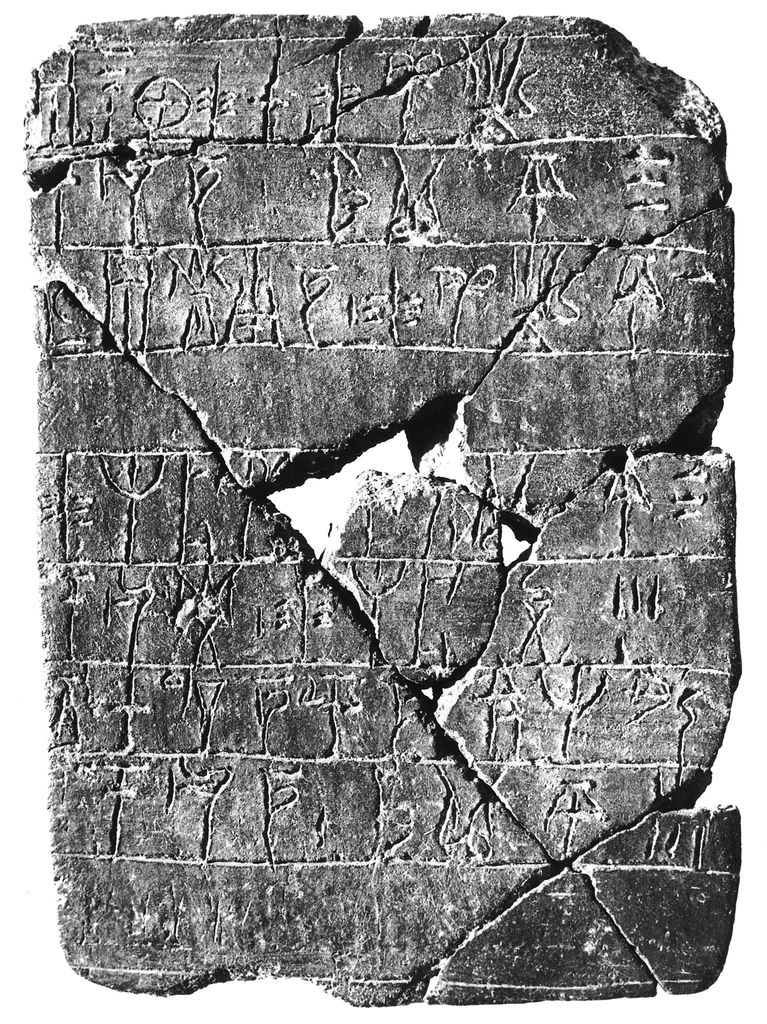
\includegraphics[width=0.38\textwidth]{Images/4959.png} % Adjust width and filename
  \caption{Picture of the original document PY Er 312.}
  \label{fig:doc9}
\end{figure}

\subsubsection{KN Fp 1+31}
This document records oil offerings made in the month of Deukios.
In this case, Tselentis provides a translation covering the whole document. \\
\textbf{Linear B text}: \textit{de-u-ki-jo-jo me-no di-ka-ta-jo di-we OLE S 1 da-da-re-jo-de OLE S 2 pa-de OLE S 1 pa-si-te-o-i OLE 1 qe-ra-si-ja OLE S 1 [...] a-mi-ni-so pa-si-te-o-i S 1 [...] e-ri-nu OLE V 3 *47-da-de OLE V 1 a-ne-mo i-je-re-ja V 4 to-so OLE 3 S 2 V 2} \\
\textbf{Greek translation}: \textgreek{Δευκίοιο μηνός: Δικταίῳ Διϝεῖ ΕΛΑΙΟΝ S 1. Δαδαλείονδε ΕΛΑΙΟΝ S 2. Πάνδει ΕΛΑΙΟΝ S 1. πασιθεοῖς ΕΛΑΙΟΝ 1. Θηρασίᾳ ΕΛΑΙΟΝ S 1 [...] Ἀμνισός: πασιθεοῖς S 1 [...] Ἐρινύι ΕΛΑΙΟΝ V 3. Οὐδαδε ΕΛΑΙΟΝ V 1. ἀνέμοιο ἱερείᾳ V 4. τόσον ΕΛΑΙΟΝ 3 S 2 V 2.} \\
\textbf{English translation}: In the month of Deukios: To Dictaean Zeus: 1 S unit of oil. To the Daedaleion: 2 S units of oil. To Pandes: 1 S unit of oil. To all gods: 1 unit of oil. To Therasia: 1 S unit of oil. [...] Amnisos: To all gods: 1 S unit (of oil). [...] To Erinys: 3 V units of oil. To Oudade: 1 V unit of oil. To the priestess of the wind: 4 V units (of oil). Total oil: 3 units, 2 S units, 2 V units.

\paragraph{Analysis.}
The translation of this document is quite accurate: the main terms and phrases are correctly rendered, and the overall structure is preserved.
This success largely reflects the document's highly regular format, which repeats the same pattern several times.

The main words that appear in this document are:
\begin{itemize}
\item \textlinb{\Bde\Bu\Bki\Bjo\Bjo} (de-u-ki-jo-jo) "of Deukios", linked to Ancient Greek \textgreek{Δευκίος}, the name of a month in the Mycenaean calendar.
This reading is confirmed by the following word \textlinb{\Bme\Bno} (me-no) "month", from Ancient Greek \textgreek{μήν}.
\item The recipients of the offerings are all in the dative case.
The first is \textlinb{\Bdi\Bka\Bta\Bjo} \textlinb{\Bdi\Bwe} (di-ka-ta-jo di-we), corresponding to Ancient Greek \textgreek{Ζεύς/Διός} with the epithet \textgreek{Δικταίος}.
The LLM associates this with Mount Dicte in Crete; Tselentis, however, writes simply "Dikatios".
\item \textlinb{\Bda\Bda\Bre\Bjo\Bde} (da-da-re-jo-de) is correctly recognized as a place-name.
The LLM renders it as the more generic "Daedaleion", while Tselentis gives "the city of Daidalos".
\item \textlinb{\BUvi\Bda\Bde} (*47-da-de) is transliterated by the LLM as "Oudade", but the initial syllabogram has no agreed phonetic value in the literature.
\item \textlinb{\Ba\Bne\Bmo} (a-ne-mo) "of the wind", from Ancient Greek \textgreek{ἄνεμος}, is correctly identified as a genitive; however, it is probably better analyzed as plural rather than singular.
\end{itemize}

In light of the above considerations, I report an improved version of both translations, highlighting in red the adjustments. \\
\textbf{Greek translation}: \textgreek{Δευκίοιο μηνός: Δικταίῳ Διϝεῖ ΕΛΑΙΟΝ S 1. Δαδαλείονδε ΕΛΑΙΟΝ S 2. Πάνδει ΕΛΑΙΟΝ S 1.} \textcolor{red}{\textgreek{πάσι θεοῖς}} \textgreek{ΕΛΑΙΟΝ 1. Θηρασίᾳ ΕΛΑΙΟΝ S 1 [...] Ἀμνισός:} \textcolor{red}{\textgreek{πάσι θεοῖς}} \textgreek{[...] Ἐρινύι ΕΛΑΙΟΝ V 3.} \textcolor{red}{\textgreek{*47-δαδε}} \textgreek{ΕΛΑΙΟΝ V 1.} \textcolor{red}{\textgreek{ἀνέμων}} \textgreek{ἱερείᾳ V 4. τόσον ΕΛΑΙΟΝ 3 S 2 V 2.} \\
\textbf{English translation}: In the month of Deukios: To Dictaean Zeus: 1 S unit of oil. To the \textcolor{red}{city of Daidalos}: 2 S units of oil. To Pandes: 1 S unit of oil. To all gods: 1 unit of oil. To Therasia: 1 S unit of oil. [...] Amnisos: To all gods: 1 S unit (of oil). [...] To Erinys: 3 V units of oil. To \textcolor{red}{?-dade}: 1 V unit of oil. To the priestess of the \textcolor{red}{winds}: 4 V units (of oil). Total oil: 3 units, 2 S units, 2 V units.

\begin{figure}[H]
  \centering
  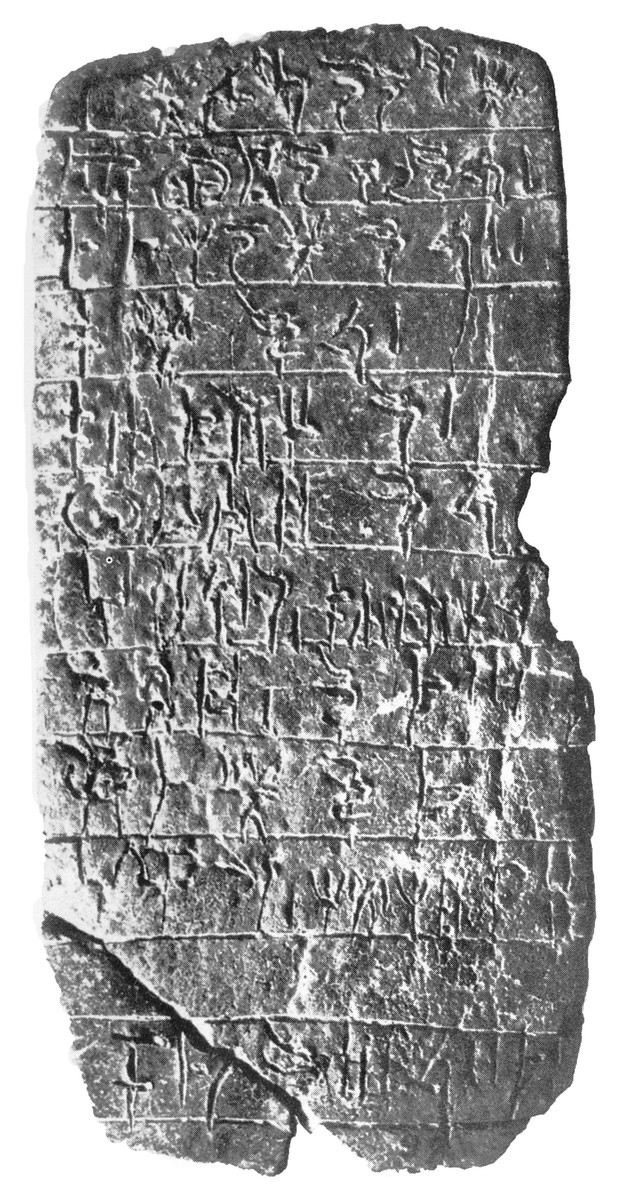
\includegraphics[width=0.38\textwidth]{Images/4088.png} % Adjust width and filename
  \caption{Picture of the original document KN Fp 1+31.}
  \label{fig:doc10}
\end{figure}

\subsubsection{PY Ab 573}
This very short document lists women and children, as well as quantities of grain and figs.
Tselentis provides a translation for a small portion of the document. \\
\textbf{Linear B text}: GRA 5 T 1 DA TA \textit{pu-ro mi-ra-ti-ja MUL 16 ko-wa 3 ko-wo 7} NI 5 1 \\
\textbf{Greek translation}: \textgreek{Πύλος: ΣΙΤΟΣ 5 T 1 DA TA. Μιλατίαι ΓΥΝΗ 16, κόρϝαι 3, κόρϝοι 7. ΣΥΚΟΝ 5 1.} \\
\textbf{English translation}: Pylos: Grain 5 T 1. DA TA. Milatian women: 16 women, 3 girls, 7 boys. Figs: 5 1.

The initial part of the document is not translated by Tselentis. It is written at the top of the tablet, as if the scribe had run out of space to complete the line.
It should probably be appended at the end of the line.
However, it is likely independent of the rest of the entry, so the LLM's placement is acceptable.

\paragraph{Analysis.}
This document is rich in logograms: the only syllabographic words are the ethnonym \textlinb{\Bmi\Bra\Bti\Bja} (mi-ra-ti-ja) from Ancient Greek \textgreek{Μιλήσιαι} "miletian", and \textlinb{\Bko\Bwo}/\textlinb{\Bko\Bwa} (ko-wo/ko-wa) from Ancient Greek \textgreek{κόρος/κόρη} "boy/girl".
The LLM correctly identifies the remaining items as logograms or abbreviations.
The translation is accurate, with a minor adjustment shown below in red. \\
\textbf{Greek translation}: \textgreek{Πύλος: ΣΙΤΟΣ 5 T 1 DA TA.} \textcolor{red}{\textgreek{Μιλήσιαι}} \textgreek{ΓΥΝΗ 16, κόρϝαι 3, κόρϝοι 7. ΣΥΚΟΝ 5 1.} \\
\textbf{English translation}: Pylos: Grain 5 T 1. DA TA. \textcolor{red}{Miletian} women: 16 women, 3 girls, 7 boys. Figs: 5 1.

\begin{figure}[H]
  \centering
  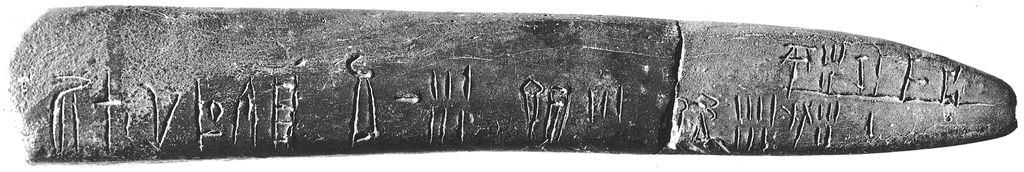
\includegraphics[width=0.7\textwidth]{Images/4611.png} % Adjust width and filename
  \caption{Picture of the original document PY Ab 573.}
  \label{fig:doc11}
\end{figure}

\subsubsection{PY Un 718} \label{doc:pyun718}
This final document is an administrative record listing offerings.
The translation provided by Tselentis for this document covers only the first part of the tablet. \\
\textbf{Linear B text}: \textit{sa-ra-pe-da po-se-da-o-ni do-so-mo o-wi-de-ta-i do-so-mo to-so e-ke-rya-wo do-se GRA 4 VIN 3 BOSm 1} tu-ryo TU+RYO 10 ko-wo *153 1 me-ri-to V 3 o-da-ha da-mo GRA 2 VIN 2 OVISm 2 TU+RYO 5 a-re-ro A+RE+PA V 2 *153 1 to-so-de ra-wa-ke-ta do-se OVISm 2 me-re-u-ro FAR T 6 VIN S 2 o-da-ha wo-ro-ki-jo-ne-jo ka-ma GRA [...] T 6 VIN S 1 TU+RYO 5 me-ri [...] 1 [...] V 1 \\
\textbf{Greek translation}: \textgreek{Σραπέδας: δόσμος Ποσειδῶνι. δόσμος οϝιδετται. Τόσος Ἐχελαϝῶν δώσει: ΣΙΤΟΣ 4, ΟΙΝΟΣ 3, ΤΑΥΡΟΣ 1, τυρίον ΤΥΡΙΟΝ 10, κοῦρος *153 1, μέλι V 3. Οδαhα δᾶμος: ΣΙΤΟΣ 2, ΟΙΝΟΣ 2, ΚΡΙΟΣ 2, ΤΥΡΙΟΝ 5. Ἀλεῖρος: ἀλειφάρ V 2, *153 1. Τοσόνδε λαϝαγέτας δώσει: ΚΡΙΟΣ 2, ἄλευρον ΦΑΡ T 6, ΟΙΝΟΣ S 2. Οδαhα ϝρογιονείον κᾶμα: ΣΙΤΟΣ [...] T 6, ΟΙΝΟΣ S 1, ΤΥΡΙΟΝ 5, μέλι [...] 1 [...] V 1.}
\textbf{English translation}: Sarapeda: Offering to Poseidon. Offering to the overseers. Echelawa will give this much: Grain 4, Wine 3, Bull 1, Cheese 10, Boy *153 1, Honey V 3. Also, the community: Grain 2, Wine 2, Ram 2, Cheese 5. Aleiros: Ointment V 2, *153 1. This much the Lawagetas will give: Ram 2, Flour T 6, Wine S 2. Also, Wrogioneios' plot: Grain [...] T 6, Wine S 1, Cheese 5, Honey [...] 1 [...] V 1.

\paragraph{Analysis.}
The LLM provides a fairly accurate translation of this document, with some problematic issues.
\begin{itemize}
  \item The first word \textlinb{\Bsa\Bra\Be\Bpe\Bda} (sa-ra-pe-da) is transliterated as "Sarapeda". The LLM considers it as a proper noun or a toponym. Its possible toponym function is mentioned also by Chadwick and Ventris in their lexicon \cite{chadwick-notes}.
  The LLM treats it as a proper noun or toponym, a possibility also noted by Chadwick and Ventris \cite{chadwick-notes}. Tselentis, however, interprets it as an epithet of Poseidon (the following word \textlinb{\Bpo\Bse\Bda\Bo\Bni} po-se-da-o-ni, \textgreek{Ποσειδῶν}) and translates "Srapedas".
  \item The word \textlinb{\Bo\Bwi\Bde\Bta\Bi} (o-wi-de-ta-i) is clearly linked to Ancient Greek \textgreek{οἶδα} "to know".
  Tselentis treats it as a religious title and leaves it transliterated; the LLM renders it as "overseers". In any case, the dative plural is correctly recognized.
  \item The verb \textlinb{\Bdo\Bse} (do-se) is correctly identified as the 3rd person singular future active indicative of the Ancient Greek verb \textgreek{δίδωμι}, "to give".
  \item A notable feature of the enumerated items in this fragment is the logographic merging of common Linear B words, which the LLM successfully reconstructs.
  For example, the word \textlinb{\Btu\Broii} (tu-ryo) appears both as a word and as the fused sign (TU+RYO) for "cheese", from Ancient Greek \textgreek{τυρίον}. 
  Conversely, \textlinb{\Ba\Bre\Bpa} (a-re-pa) appears only as the logogram (A+RE+PA) for "ointment", from Ancient Greek \textgreek{ἀλείφαρ}.
  \item The meaning of \textlinb{\Bko\Bwo}, paired with the unknown syllabogram *153, is uncertain.
  \item \textlinb{\Bo\Bda\Baii} (o-da-ha) is treated as a conjunction "also", which matches Tselentis' description as an introductory word.
  \item \textlinb{\Bwo\Bro\Bki\Bjo\Bne\Bjo} \textlinb{\Bka\Bma} (wo-ro-ki-jo-ne-jo ka-ma) refers again to the Worgiones cult association, as in Document \hyperref[doc:pyer312]{PY Er 312}.
  \textit{ka-ma} is correctly taken as "plot/field", from Ancient Greek \textgreek{κτῆμα}.
\end{itemize}

Here I report a refined version of both translations, highlighting in red the adjustments. \\
\textbf{Greek translation}: \textgreek{Δόσμος} \textcolor{red}{\textgreek{Σραπέδᾳ}} \textgreek{Ποσειδῶνι. Δόσμος} \textcolor{red}{\textgreek{οϝιδέταις}}\textgreek{. Τόσος Ἐχελαϝῶν δώσει: ΣΙΤΟΣ 4, ΟΙΝΟΣ 3, ΤΑΥΡΟΣ 1, τυρίον ΤΥΡΙΟΝ 10, κοῦρος *153 1, μέλι V 3. Οδαhα δᾶμος: ΣΙΤΟΣ 2, ΟΙΝΟΣ 2, ΚΡΙΟΣ 2, ΤΥΡΙΟΝ 5. Ἀλεῖρος: ἀλειφάρ V 2, *153 1. Τοσόνδε λαϝαγέτας δώσει: ΚΡΙΟΣ 2, ἄλευρον} \textcolor{red}{\textgreek{ΑΛΕΥΡΟΝ}} \textgreek{T 6, ΟΙΝΟΣ S 2. Οδαhα} \textcolor{red}{\textgreek{ϝοργιονείον κτῆμα}}\textgreek{: ΣΙΤΟΣ [...] T 6, ΟΙΝΟΣ S 1, ΤΥΡΙΟΝ 5, μέλι [...] 1 [...] V 1.} \\
\textbf{English translation}: Offering to \textcolor{red}{Srapedas} Poseidon. Offering to the overseers. \textcolor{red}{Echelawon} will give this much: Grain 4, Wine 3, Bull 1, Cheese 10, Boy *153 1, Honey V 3. Also, the community: Grain 2, Wine 2, Ram 2, Cheese 5. Aleiros: Ointment V 2, *153 1. This much the Lawagetas will give: Ram 2, Flour T 6, Wine S 2. Also, the plot \textcolor{red}{of the Worgiones}: Grain [...] T 6, Wine S 1, Cheese 5, Honey [...] 1 [...] V 1.

\begin{figure}[H]
  \centering
  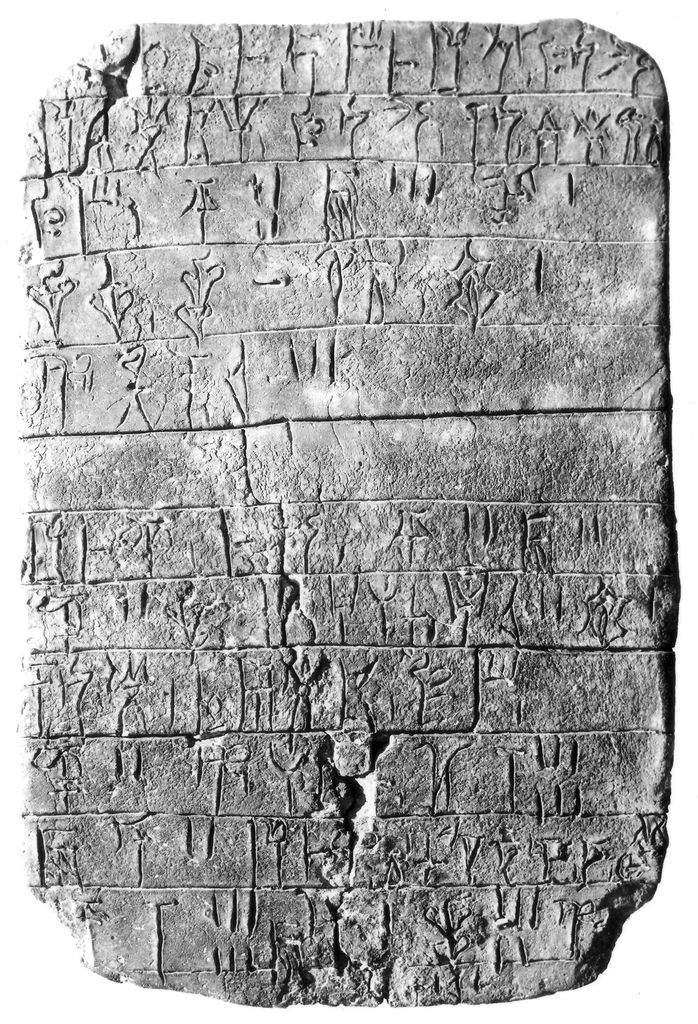
\includegraphics[width=0.45\textwidth]{Images/5385.png} % Adjust width and filename
  \caption{Picture of the original document PY Un 718.}
  \label{fig:doc12}
\end{figure}

The translations of all remaining documents are provided in the thesis files, in a CSV file that includes the document index, the Linear B form, the Greek and English translations, and the model's reasoning.

\subsection{Error Analysis} \label{sec:errors}
This section summarizes the errors made by the LLM in translating the selected documents and analyzes their likely causes, given the input information.

The first type of error arises from misinterpreting words when cognate support is insufficient or misleading.
This is especially likely when no clear Ancient Greek cognate exists or when the cognate's meaning has shifted.
For example, in Document \hyperref[doc:pyjn310]{Py Jn 310} the form \textlinb{\Bpo\Bti\Bni\Bja\Bwe\Bjo} (po-ti-ni-ja-we-jo) is not treated as place-related, because Ancient Greek \textgreek{πότνια} ("mistress/lady") no longer transparently denotes a deity.
Another example appears in Document \hyperref[doc:knso4439]{KN So 4439}, where \textlinb{\Be\Bri\Bka} (e-ri-ka) is associated with Ancient Greek \textgreek{ἑλικτός} "twisted", unlike in Linear B, where it is associated with the willow tree.

A second type of error is the misinterpretation of a word's grammatical function.
This can occur when the LLM fails to recognize a noun's case or a verb's tense.
For instance, in document \hyperref[doc:pyan657]{PY An 657}, \textlinb{\Be\Bra\Bwo} (e-ra-wo) is treated as a nominative noun, whereas it is actually genitive.
Another example is in document \hyperref[doc:pyta641]{PY TA 641}, where \textlinb{\Bke\Bre\Baii} (ke-re-ha), from Ancient Greek \textgreek{σκέλεα} "legs", is not associated with its particle \textgreek{ἀπό}; however, this error is likely attributable to the unusual placement of the initial line in the document.

The third error type I want to highlight is the misinterpretation of a word's function due to misclassification.
When the auxiliary classifiers mislabel a word, the LLM may misassign its role in the sentence.
For example, in Document \hyperref[doc:pyan657]{PY An 657}, two ordinary locatives are interpreted as proper toponyms: both \textlinb{\Bo\Bpi\Baii\Bra} (o-pi-ha-ra) and \textlinb{\Bri\Bme\Bne} (ri-me-ne) are rendered as "Opihara" and "Limenei", rather than "at the coast" and "at the port".
Likewise, the two occurrences of \textlinb{\Bwo\Bro\Bki\Bjo\Bne\Bjo} (wo-ro-ki-jo-ne-jo) in Documents \hyperref[doc:pyer312]{PY Er 312} and \hyperref[doc:pyun718]{PY Un 718} are misclassified as a proper name, which leads to an interpretation as an anthroponym rather than as a cult association.

Finally, some errors arise from the LLM's difficulty in interpreting certain logographic abbreviations, which are occasionally misread or left unspecified.
Taken together, these are the main error patterns observed in the analyzed documents, given the input information available to the model.

A further, notable issue is the LLM's tendency to produce forms closer to Mycenaean than to classical Ancient Greek.
Many translations retain clear Linear B reminiscences, most notably the persistent use of the digamma (\textgreek{ϝ}) and frequent Mycenaean case endings.
I have largely set these aside when the sense was clear and the content was correctly interpreted.
However, if classical Ancient Greek is to serve as a reliable support language for translation, the system will need better normalization toward Classical morphology and orthography (e.g., consistent suppression of \textgreek{ϝ} where appropriate and alignment with Classical inflectional endings).
\chapter{Conclusions and Future Work} \label{chap:conclusion}

\section{Conclusion}
Overall, the analysis of the errors made by the LLM in interpreting the selected Linear B documents demonstrates that automated translation is indeed feasible. The most important elements of the tablets are generally identified and rendered correctly, especially when the documents exhibit regular, list-like structures and well-attested administrative formulas.
Across the analyzed documents, the model typically reconstructs the local context, constrains its lexical choices to domain-appropriate vocabulary, and produces English glosses that capture the intended sense.

That said, some sources of error are inherent to the writing system.
The tablets are highly contracted and context-poor; many entries admit multiple plausible interpretations.
As outlined in Section \ref{sec:errors}, the most frequent failure mode is the misinterpretation of grammatical case or number, often triggered by overlapping Linear B endings and sparse syntactic cues.
Additional errors arise when auxiliary classifiers mislabel the function of a form or when logograms and abbreviations are only partially disambiguated.

A further systematic issue concerns the Ancient Greek reconstructions.
The LLM often retains Mycenaean features (e.g., persistent \textgreek{ϝ}, Mycenaean endings), which makes some outputs less than fully classical.
Crucially, however, these deviations rarely obscure the core semantics.
The English translations, the ultimate target for accessibility and cross-document comparison, remain largely accurate even when the Greek layer is not perfectly normalized.
In this sense, the pipeline already serves as a practical aid: it accelerates first-pass interpretation, surfaces consistent readings for recurring formulas, and makes tablets more accessible to readers without specialist training in Mycenaean Greek or Linear B paleography.
At the outset of this project, a tool of this kind would have significantly accelerated my own work by providing reliable preliminary translations to inspect and refine.

In conclusion, while there is clear room for improvement, particularly in normalizing Greek forms toward Classical conventions, strengthening grammatical disambiguation, and refining logogram handling, the LLM-based system demonstrates substantial promise.
It delivers dependable, high-coverage drafts that scholars can validate and adjust, supports hypothesis generation about uncertain forms, and lowers the entry barrier for broader audiences.
With incremental enhancements to auxiliary signals and normalization, the approach can mature into a robust companion for philological analysis and digital editions of Linear B texts.

\section{Future Work}

Building on the encouraging results of this initial exploration, several avenues for future work emerge.
Expanding the auxiliary classifiers to cover additional grammatical categories (e.g., tense, mood, and voice for verbs; degree for adjectives; case, number, and gender for nouns and adjectives) could help the LLM better disambiguate forms with overlapping endings.
The classifier datasets could be manually reviewed and corrected to improve accuracy, since they were synthesized via automated prompt-engineering (Section~\ref{sec:aux-dataset}).
As these labels guide the LLM's choices, improving them should propagate to more reliable reconstructions.
Similarly, enhancing the disambiguation of logographic abbreviations with a more comprehensive, context-aware lexicon could further improve the model's performance.

Other potential improvements include:
\begin{itemize}
\item \textbf{Domain adaptation and fine-tuning.} Fine-tune the LLM on a curated corpus of Linear B texts paired with expert-validated Greek and English translations to internalize domain-specific formulae and genre constraints while reducing over-generalization from non-administrative Greek.

\item \textbf{Normalization toward Classical Greek.} Add a dedicated normalization stage that maps Mycenaean-like outputs to Classical morphology and orthography, implemented either as a post-processing transducer constrained by paradigms or as a jointly trained module with soft constraints for the suppression of \textgreek{ϝ} and alignment to Classical endings.  

\item \textbf{Richer cognate modeling.} Evolve the Cognate Matching model and framework by incorporating explicit phonological and inflection-aware correspondences.

\item \textbf{Better handling of logograms and abbreviations.} Expand the logogram lexicon with contextual priors (e.g., commodity-unit co-occurrence, site-specific practices), and integrate a small decision model that prefers readings consistent with neighboring quantities and roles.  

\item \textbf{Cross-script generalization.} Experiment with related scenarios where closely related languages are encoded in different scripts (e.g., Cypriot syllabary and alphabetic Greek) to test the portability of the pipeline beyond Linear B.  
\end{itemize}

Finally, a more systematic evaluation over a larger and more diverse set of Linear B documents would better quantify strengths and weaknesses and guide refinement.
The same methodology could then be extended to other ancient languages and scripts, testing the generalizability of the approach.

All data and code used in this thesis are available on GitHub at \url{https://github.com/SirAlex01/LALB-DM-Project}.

Open sourcing any Linear B resources is particularly important, given the scarcity of digital tools for this script and the limited accessibility of many primary sources.


\backmatter
\cleardoublepage
\phantomsection % Give this command only if hyperref is loaded
\addcontentsline{toc}{chapter}{\bibname}
% Here put the code for the bibliography. You can use BibTeX or
% the BibLaTeX package or the simple environment thebibliography.

\printbibliography

\end{document}